\documentclass[12pt, letterpaper]{article}
\usepackage{graphicx} % Required for inserting images
\usepackage{hyperref}
\usepackage[table,xcdraw]{xcolor}
\usepackage{amssymb}
\usepackage{amsmath}
\usepackage[english]{babel}
\usepackage{nicefrac, xfrac}
\usepackage{tikz}
\newcommand{\K}{{\mathbb K}}
\newcommand{\Z}{{\mathbb Z}}
\newcommand{\R}{{\mathbb R}}
\newcommand{\N}{{\mathbb N}}
\newcommand{\Sn}{{\mathcal S_n}}
\newcommand{\An}{{\mathcal A_n}}
\newcommand{\E}{{\mathcal E}}
\newcommand{\B}{{\mathcal B}}
\newcommand{\dimo}{{\text{\textbf{Dimostrazione }:}}}
\newcommand{\mcm}{{\text{mcm}}}
\newcommand{\rg}{{\text{rg}}}
\newcommand{\ve}{{\bar v}}
\newcommand{\spaz}{{\text{\hphantom{aa}}}}
\newcommand{\MCD}{{\text{MCD}}}
\newcommand{\supp}{{\text{Supp}}}
\newcommand{\acc}{\\\hphantom{}\\}
\newcommand{\aut}{{\text{Aut}}}
\newcommand{\Span}{{\text{Span}}}
\newcommand{\End}{{\text{End}}}
\newcommand{\cen}{{\text{Centro}}}
\newcommand{\norm}{{\unlhd}}
\newcommand{\ciclS}{{\left \langle }}
\newcommand{\ciclE}{{\right \rangle }}
\newcommand{\boxedMath}[1]{\begin{tabular}{|c|}\hline \texttt{#1} \\ \hline\end{tabular} :}
\usetikzlibrary{positioning}
\usepackage[paper=a4paper,left=20mm,right=20mm,bottom=25mm,top=25mm]{geometry}
\title{Algebra}
\author{Marco Casu}
\date{\vspace{-5ex}}
\begin{document}
\newcommand{\omo}[1]{\(\varphi\)}


\maketitle
\begin{figure}[h]
    \centering{
    
\includegraphics[width=0.8\textwidth ]{images/Copertina2.png}
    }
\end{figure}
\newpage 
\tableofcontents
\newpage
\section{Insiemi e Relazioni}
Sappiamo già che un insieme non è altro di una collezione di oggetti distinti.\raggedright\\
\centering
\(A=\{1,2,3,4,5\}\)\\
\raggedright
Ricapitoliamo le proprietà basiche degli insiemi : 
\begin{itemize}
    \item \textbf{Intersezione} - \(A \cap B \rightarrow \{x | x\in A \land x\in B\}\)
    \item \textbf{Unione} - \(A \cup B \rightarrow \{x | x\in A \lor x\in B\}\)  
    \item \textbf{Sottoinsieme} - \(A \subseteq B \rightarrow  \{x\in A \implies x \in B\}\)
    \item \textbf{Insieme complementare} - \(A^c_{\text{in B}} \rightarrow \{x\in B | x \notin A\}\)
\end{itemize}
\subsection{Proprietà fondamentali degli insiemi}
Elenchiamo le già note proprietà degli insiemi :
\begin{itemize}
    \item \textbf{Associativa} - \( (A \cap B)\cap C =  (C \cap B)\cap A \)  oppure   \( (A \cup B)\cup C =  (C \cup B)\cup A \)
    \item \textbf{De Morgan} - Se \(A, B \subseteq C\) allora \((A \cap B)^c = A^c \cup B^c\) oppure \((A \cup B)^c = A^c \cap B^c\) 
    \item \textbf{Distributiva} - \( (A\cup B)\cap C = (A \cap C)\cup(B \cap C)  \) oppure \( (A\cap B)\cup C = (A \cup C)\cap(B \cup C)  \)
\end{itemize}
Un insieme particolare associato ad un dato insieme \(A\) è \textbf{l'insieme delle parti} di \(A\),
è l'insieme di tutti i possibili sotto-insiemi di \(A\) e si indica con :
\begin{equation}
    \mathcal{P}(A) = \{ B | B \subseteq A \}
\end{equation}
\\Introduciamo adesso il concetto di \textbf{prodotto cartesiano} su due insiemi \(A\) e \(B\),
 esso non è altro che l'insieme di tutte le coppie ordinate dove il primo elemento appartiene ad \(A\)
 ed il secondo elemento a \(B\) :
 \begin{equation}
    A \times B = \{ (a,b) | a\in A, b\in B\}
 \end{equation}
\subsection{Le Relazioni}
Una relazione \(\rho\) da un insieme \(A\) ad un insieme \(B\), è un sotto-insieme del prodotto
cartesiano \( A \times B\).
\begin{equation}
    \rho \subseteq A \times B \text{,  se } (a,b)\in \rho \text{ si scrive }a\rho b
\end{equation}
Il dominio di tale relazione \(\rho\) risulta essere :
\begin{equation}
    \mathcal{D}(\rho)=\{a\in A | \exists b\in B \text{ per il quale risulti }a\rho b\}
\end{equation}
La sua immagine : 
\begin{equation}
    \Im(\rho)=\{b\in B | \exists a\in A \text{ per il quale risulti }a\rho b\}
\end{equation}
Per una relazione \(\rho\), se il suo dominio risulta essere tutto \(A\), e 
\(\forall a\in A \exists \text{ un unico } b \in B | a\rho b\), tale \(\rho\) è 
anche una \textbf{funzione}.
\\\textit{Esempio di relazione : }\\
sia \(A=\{a,b,c,d\}\), è definita la relazione \(\rho \subseteq A\times A = \{(a,b),(b,c),(c,c),(c,a),(d,b)\}\).
\newpage Abbiamo due modi per poter visualizzare una relazione, un formato tabellare, ed un formato 
con nodi e collegamenti fra gli elementi della relazione. Per la relazione \(\rho \) appena enunciata si ha la seguente rappresentazione tabellare
dove si inserisce un 1 nel punto in cui le due coordinate sono in relazione fra loro : 
\\ \hphantom{.}\\
\centering
\begin{tabular}{ c c c c c }
    \(d\) & 0 & 0 & 0 & 0  \\ 
    \(c\) & 0 & 1 & 1 & 0  \\ 
    \(b\) & 1 & 0 & 0 & 1  \\ 
    \(a\) & 0 & 0 & 1 & 0  \\ 
    &\(a\) & \(b\) & \(c\) & \(d\) 
        
   \end{tabular}
\\ 
 \hphantom{.}\\
 \raggedright
Vediamone adesso una rappresentazione con nodi e collegamenti : 
 \\
 \centering
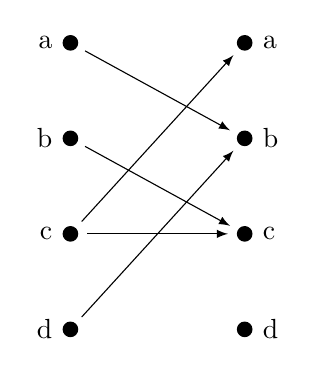
\begin{tikzpicture}[
    mydot/.style={
      circle,
      fill,
      inner sep=2pt
    },
    >=latex,
    shorten >= 3pt,
    shorten <= 3pt
    ]
    \node[mydot,label={left:a}] (a1) {}; 
    \node[mydot,below=of a1,label={left:b}] (a2) {}; 
    \node[mydot,below=of a2,label={left:c}] (a3) {}; 
    \node[mydot,below=of a3,label={left:d}] (a4) {}; 
    
    \node[mydot,right=2cm of a1,label={right:a}] (b1) {}; 
    \node[mydot,below=of b1,label={right:b}] (b2) {}; 
    \node[mydot,below=of b2,label={right:c}] (b3) {}; 
    \node[mydot,below=of b3,label={right:d}] (b4) {}; 
    
    \path[->] (a1) edge (b2);
    \path[->] (a2) edge (b3);
    \path[->] (a3) edge (b1)
      edge (b3);
    \path[->] (a4) edge (b2) ;
    
    \end{tikzpicture}
    \\ 
 \raggedright
 Essendo le relazioni degli insiemi, possiamo considerare le operazioni di unione ed intersezione
 anche per le relazioni. Esista per ogni relazione, anche la sua \textbf{relazione inversa},
 se \(\rho\) è definita da \(A\) a \(B\), esisterà \(\rho^{-1}\) definita da \(B\) a \(A\).
 \begin{equation}
    \rho^{-1} = \{ (b,a) \in B\times A | a\rho b\} \text{ quindi } a\rho b \implies b\rho^{-1} a
 \end{equation}
 Se la relazione \(\rho\) è una funzione, non è detto che la sua relazione inversa sia una funzione anch'essa,
 prendiamo ad esempio la relazione \(\rho \subset \mathbb{R} \times \mathbb{R}  =\{ (x,x^2) \forall a\in \mathbb{R}\}\), che non è altro che
 la funzione di una variabile reale \(f(x)=x^2\). Tale funzione, per \(x=-a\) ed \(x=a\), ha sempre \(f(x)=a^2\), per due valori
 appartenti al dominio ha la stessa immagine, la sua funzione inversa avrebbe quindi un punto che mappa due immagini.
\\\hphantom{.}\\
Una relazione nota su insieme \(A\) è la \textbf{relazione identità}, definita : \(\Delta_A = \{(a,a)\in A \times A\}\).
\subsection{Relazioni di Equivalenza}
Una relazione \(\rho\) definita su un insieme \(A\), quindi \(\rho \subseteq A \times A\), è detta \textbf{relazione 
di equivalenza} se soddisfa i seguenti requisiti : 
\begin{itemize}
    \item \(\rho\) è \textbf{riflessiva}, ossia è vero che :  \(a\rho a \forall a \in A\)
    \item \(\rho\) è \textbf{simmetrica}, ossia è vero che se esiste \(a\rho a'\) allora esiste \(a'\rho a\)
    \item \(\rho\) è \textbf{transitiva}, se esistono \(a\rho a'\) e \(a'\rho a''\), allora esiste \(a\rho a''\)
\end{itemize}
Un esempio di relazione di equivalenza è la relazione di \textit{avere la stessa età} su un 
insieme di studenti, difatti soddisfa tutti e 3 i requisiti : 
\begin{itemize}
    \item è \textbf{riflessiva} perchè ognuno ha la stessa età di se stesso.
    \item è \textbf{simmetrica} perchè se tizio ha la stessa età di caio, caio ha la stessa età di tizio.
    \item è \textbf{transitiva} perchè se tizio ha la stessa età di caio e caio ha la stessa età di sempronio, tizio ha la stessa età di sempronio.
\end{itemize}\newpage
Un esempio di relazione \textbf{non} di equivalenza è la relazione di \textit{genitorialità}, ad esempio non è simmetrica, perchè se 
tizio è padre di caio, caio non è assolutamente padre di tizio.
\subsection{Le Classi di Equivalenza}
Sia \(\rho\) una relazione di equivalenza definita su \(A\), si definisce \textbf{classe di equivalenza} di un 
elemento \(a\in A\), e si denota con \([a]\), l'insieme di tutti gli elementi di \(A\) che sono equivalenti (ossia in relazione di 
equivalenza) ad \(a\), ossia 
\begin{equation}
    [a] = \{b\in A | b\rho a\}
\end{equation}
Ad esempio, su una relazione di \textit{avere la stessa età}, in ogni classe di equivalenza ci sono tutte le persone
che hanno la stessa età : ogni classe può essere quindi un etichetta con il numero corrispondente all'età.
\\ \textit{Esempio esteso : }\\
Si prenda in considerazione il seguente insieme di persone :\\\centering \(A=\{\)Valentino,Marco,Luca,Alessandro,Davide\(\}\)\\
\raggedright
Ognuno ha i seguenti anni : 
\begin{itemize}
    \item Valentino - 20
    \item Marco - 19
    \item Luca - 20
    \item Alessandro - 19
    \item Davide - 19
\end{itemize}
La relazione di \textit{avere la stessa età} su \(A\) è definita come :\\ \(\rho=\{(Valentino,Luca),(Luca,Luca),(Marco,Alessandro),(Alessandro,Davide)...ecc\}\)
\\La classe di equivalenza \([Marco]=\{Marco,Alessandro,Davide\}\) definisce tutti gli elementi in relazione con \(Marco\), e rappresenta
tutte le persone di età uguale a 19.\\\hphantom{.}\\
Sia \(A\) un insieme sulla quale è definita una relazione di equivalenza, l'insieme \(\nicefrac{A}{a}\) è detto 
\textbf{insieme quoziente}, ed è l'insieme che contiene tutte le classi di equivalenza della relazione definita su \(A\).
\begin{equation}
    \nicefrac{A}{a}=\{[a], a\in A\}
\end{equation}
Vediamo adesso un \textbf{importante proprietà} delle classi di equivalenza : 
\newtheorem{theorem}{Teorema}
\begin{theorem}
\begin{equation}
    [a]=[b] \iff a\rho b
\end{equation}
\end{theorem}
\newtheorem{dimostrazione}{Dimostrazione}
\begin{dimostrazione}
    Ovviamente \(b\in [b]\) perchè \(b\rho b\), essendo  \([a]=[b] \implies b \in [a]\implies b\rho a\implies a\rho b\),
    Analogamente, se \(a\rho b\), se esiste \(c \in [a]\implies c\rho a \implies c \rho b \implies c\in [b]\implies
    [a]\subseteq[b]\).\\
    se esiste \(c \in [b]\implies c\rho b \implies c \rho a \implies c\in [a]\implies
    [b]\subseteq[a]\). Essendo \( [b]\subseteq[a]\) e \( [a]\subseteq[b]\), per forza di cose \([a]=[b]\).
\end{dimostrazione}
\raggedleft\(\blacksquare\)\newpage
\raggedright \subsubsection{Le Partizioni}
Dicesi \textbf{partizione} di un insieme \(A\) una \textit{collezione di parti o sotto-insiemi} \(A_\alpha\) non 
vuoti di \(A\) tali che \textbf{l'unione} di tutti i sotto-insiemi sia \(A\), ossia, tali collezioni \textit{ricoprono} \(A\).
\begin{equation}
    \bigcup_\alpha A_\alpha = A 
\end{equation}
Ciò significa che \(A_\alpha \cap A_\beta \ne \varnothing \implies A_\alpha = A_\beta\), in un linguaggio meno formale, tutte le partizioni 
di un insieme \(A\), non condividono nessun elemento di \(A\). Nell'immagine seguente, \(A'\) e \(A''\) sono partizioni di \(A\).
\begin{figure}[h]
    \centering{
    \includegraphics[width=0.35\textwidth ]{images/partition.eps}
    }
\end{figure}
\newtheorem{prop}{Proposizione}
\begin{prop}
    Sia \(\rho\) una relazione di equivalenza su \(A\), le classi di equivalenza di \(\rho\) sono
    partizioni di \(A\).
\end{prop}
\textit{Dimostrazione}:\\
    Ricoprono totalmente \(A\), essendo \(a \rho a \forall a \in A\), ogni \(a\) appartiene alla sua classe 
    di equivalenza.  Inoltre le classi di equivalenza, o coincidono o sono disgiunte.
\begin{prop}
    Ogni partizione di un insieme \(A\) determina su \(A\) una relazione di equivalenza, per la quale i sotto insiemi
    della partizione sono le classi di equivalenza.
\end{prop}
\textit{Dimostrazione}:\\
Se indichiamo con \(B_\alpha\) i sotto-insiemi della partizione \(A_\alpha\) su \(A\), è ovvio che :
\begin{equation}
    a\rho b \implies \exists B_\alpha | a,b \in B_\alpha
\end{equation}
Una relazione di equivalenza definisce a sua volta delle classi di equivalenza, che definiscono a loro volta delle partizioni.
\subsection{Relazioni di Ordine Parziale}\label{ordParz}
Introduciamo adesso un'altro gruppo di relazioni, ma prima necessitiamo della definizione di \textbf{relazione antisimmetrica} :
\begin{equation}
    \text{Sia }\rho \text{ una relazione, essa si dice \textbf{antisimmetrica} se è vero che } a\rho b \text{ e } b\rho a \implies a=b 
\end{equation}
Detto ciò, possiamo definire una \textit{relazione di ordine} parziale se essa è :\begin{itemize}
    \item Riflessiva
    \item Transitiva
    \item Antisimmetrica
\end{itemize}
\textit{Esempio 1} - Sia \(X\) un insieme, e sia \(\mathcal{P} (X)\) l'insieme delle sue parti, definiamo 
la relazione sugli elementi di \(\mathcal{P} (X)\) nel seguente modo \(\rho = \{\{A,B\} \text{ con } A,B\in\mathcal{P}(X) \text{ se } A\subseteq B\}\),
quindi \(A\rho B \iff A\subseteq B\), è chiaro che tale relazione soddisfa i 3 requisiti, è quindi 
di ordine parziale.\\\hphantom{.}\\
\textit{Esempio 2} - Prendiamo come relazione la divisibilità in \(\mathbb{N}\text{*} = \mathbb{N}\backslash \{0\}\)  
, siano \(a,b \in \mathbb{N}\text{*}\) vale che \(a\rho b\iff a | b\), dove \(a|b\) significa \textit{ \(a\) divide \(b\)},
ossia che \(\exists x \in \mathbb{N}\text{*} \text{ tale che } b=a\cdot x\). Tale relazione è di ordine parziale 
dato che è riflessiva (\(a=1\cdot a\) quindi \(a\rho a\)), è transitiva (dato che se \(a\) è divisibile per \(b\)
e \(b\) è divisibile per \(c\), è ovvio che \(a\) sia divisibile per \(c\)), e risulta essere anche 
antisimmetrica, dato che : 
\begin{equation}
     \begin{cases} 
        a\rho b\\
        b\rho a 
     \end{cases}
     \implies 
     \begin{cases} 
        b=ax\\
        a=by 
     \end{cases}
     \implies a = (ax)y \implies xy = 1
\end{equation}
Quando si ha una relazione di ordine parziale, gli elementi di tale relazione godono della proprietà 
di poter essere rappresentati graficamente in un determinato modo, ma prima di enunciare tale rappresentazione,
necessitiamo di una definizione.
\begin{theorem}
    Sia \(\rho\) una relazione d'ordine parziale su un insieme \(A\), presi \(a,b \in A\), diciamo che 
    \(a\) \textbf{è coperto} da \(b\) e scriveremo \begin{equation}
        a\preccurlyeq b
    \end{equation}
    se \(a\rho b \) e non esiste nessun elemento \(c\) tale che \(a\rho c \) e \(c \rho b\).
\end{theorem}
Ad esempio, prendiamo l'insieme \(A  = \{1,2,3,5,6.10,15,30\}\), ossia dei numeri naturali che dividono \(30\).
Risulta chiaro come :
\begin{itemize}
    \item \(2 !\preccurlyeq 30\) 30 non è il primo valore che si fa 
    dividere da 2, ci sono valori prima di 30 per il quale 2 è divisore.
    \item \(2 !\preccurlyeq 3\) dato che 2 e 3 non sono nemmeno in relazione.
    \item \(2 \preccurlyeq 6\) perchè 6 è il primo numero che 2 può dividere. 
\end{itemize}
Stabilito ciò, possiamo \textit{rappresentare graficamente} una relazione di ordine parziale su un 
insieme finito tramite il \textbf{diagramma di Hasse}, disegnando tutti gli elementi dell'insieme, 
collegandoli con una fraccia ogni dove un elemento \textit{copre} un altro.
\\ \begin{center}
    preso \(A=\{1,2,3,5,6.10,15,30\}\) e la relazione di divisibilità prima enunciata, si ha
\end{center}
\begin{figure}[h]
    \centering{
    \includegraphics[width=0.75\textwidth ]{images/hassDivisibilità.eps}
    }
\end{figure}
\newpage
\subsection{I Numeri Naturali}
Dalle scuole elementari siamo abituati a lavorare e fare operazioni con i numeri naturali, in questa 
sezione ne daremo una definizione assiomatica in termini di \textit{fondamenti della matematica}.
È importante in questo
momento non considerare assolutamente il concetto di numeri naturali che ci è ben chiaro, e cercare di leggere il seguente 
paragrafo da un punto di vista puramente logico, dando nulla per scontato.
\subsubsection{La Terna di Peano}
Introduciamo prima quella che è un'astrazione dei numeri naturali, ossia la \textbf{terna di Peano}. 
\begin{equation}
    (\mathbb{N} ,\sigma ,0)
\end{equation}
Si indica in questo caso con \(\mathbb{N}\) un insieme di elementi, non i numeri naturali alla quale siamo abituati,
con \(\sigma\) invece si indica una funzione \(\sigma : \mathbb{N}\rightarrow\mathbb{N}\),
e dato ogni elemento \(n\in \mathbb{N}\), l'elemento \(\sigma(n)\) si dice \textit{successivo} di \(n\).  Su tale terna, sono definiti 
3 fondamentali assiomi : 
\begin{itemize}
    \item \(\mathbb{N}_1\) - \(\sigma\) è una funzione iniettiva.
    \item \(\mathbb{N}_2\) - \(0 \notin \Im(\sigma)\), 0 non è contenuto nell'immagine di \(\sigma\).
    \item \(\mathbb{N}_3\) (\textit{Principio di induzione matematica}) - Se \(U\subseteq\mathbb{N}\), ed è vero che :
    \begin{itemize}
        \item\(0\in U\)
        \item\(k\in U \implies \sigma(k)\in U\)
    \end{itemize}
    Allora \(U=\mathbb{N}\)
    \\\hphantom{.}\\\textit{Dimostrazione}\\
    Considero \(U=\{0\}\cup\{n|\exists n' \text{ tale che }\sigma(n')=n\}\) quindi \(k\in U \implies \exists k' | k=\sigma(k')\)
     allora risulta ovvio che \(\sigma(k)=\sigma(\sigma(k')) \in U \implies U = \mathbb{N} \).
\end{itemize}
\subsubsection{Definizione Formale}
Dati tali assiomi adesso procesiamo nel riconnetterci con l'insieme dei numeri naturali da noi conosciuti,
enunciandone le proprietà elementari secondo la terna di Peano.\\
Sia \((\mathbb{N} ,\sigma ,0)\) una terna di Peano, presi \(n,m \in \mathbb{N}\), dirò che \(n\le m \iff m = \sigma(\sigma(\sigma(...n)))\),
ossia che \(n\) è minore o uguale di \(m\) se \(m\) è uguale a \(\sigma\) applicato su \(n\) un certo numero di volte. 
\begin{quote}
    \textbf{Proposizione} - Questo stabilisce una relazione di ordine totale.
\end{quote}
Adesso definiamo le operazioni elementari che conosciamo sui numeri naturali, ossia di somma e prodotto.\\
Definiamo la \textbf{somma} come operazione su un insieme \(\mathbb{N} \times \mathbb{N} \rightarrow\mathbb{N}\), ossia che 
associa ad ogni coppia di elementi di \(\mathbb{N}\), un elemento di \(\mathbb{N}\).
\begin{equation}
    n,m\in \mathbb{N}\text{ si definisce somma } n\times m \rightarrow n+m
\end{equation}
La somma è definita in tal modo :
\begin{itemize}
    \item (i) \(0+b=b\)
    \item (ii) \(\sigma(a)+b=\sigma(a+b)\)
\end{itemize}
\begin{quote}
    \textbf{Osservazione} - \(\sigma(0)+b = \sigma(0+b)=\sigma(b)\),
    Se poniamo \(\sigma(0)=1\), allora vediamo che \(\sigma(b)=b+1\).
\end{quote}
Definamo adesso il \textbf{prodotto}, sempre come un operazione \(\mathbb{N} \times \mathbb{N} \rightarrow\mathbb{N}\)
avente le seguenti proprietà :
\begin{itemize}
    \item (i) \(0\cdot b=0 \forall b\in \mathbb{N}\)
    \item (ii) \(\sigma(a)\cdot b = a\cdot b +b\)
\end{itemize}
\begin{quote}
    \textit{Si può dire che gli assiomi di Peano caratterizzano i numeri naturali. Quello che si deve 
    accettare senza dimostrazione, è l'esistenza di un insieme \(\mathbb{N}\) verificante gli
    assiomi di Peano.}
\end{quote}
\section{I Numeri Interi}
Nell'insieme \(\mathbb{N}\), non ci è permesso risolvere \(x+1=0\). In questo capitolo partiremo dai numeri 
naturali per costruirne un estensione in grado di rappresentare gli interi. Partendo dal prodotto cartesiano 
\(\mathbb{N}\times\mathbb{N}\), costruiamo una relazione del tipo : 
\begin{equation}
    (n,m)\sim (n',m')\iff n+m' = m+n'
\end{equation}
In linguaggio meno formale, una coppia \((0,a)\) è in relazione con tutte le coppie \(n,m\), per cui \(n-m=-a\),
ed  una coppia \((a,0)\) è in relazione con tutte le coppie \(n,m\), per cui \(n-m=a\).\\
\textit{Esempio :}
\begin{center}
    \((5,6)\sim (0,1)\iff 5+1 = 6+0 \)\\\((8,2)\sim (6,0)\iff 8+0 = 2+6\)
\end{center}
Si nota facilmente come tale relazaione sia di equivalenza, possiamo quindi definire delle classi di equivalenza
che ripartiscono l'insieme \(\mathbb{N}\times\mathbb{N}\) in classi \([(n,m)]\). Scegliamo come \textit{rappresentanti}
delle classi di equivalenza gli elementi che prevedono uno dei due elementi uguale a \textit{zero}, ogni classe sarà 
rappresentabile con uno dei seguenti rappresentanti distinti :
\begin{center}
    \((0,0)\)\hphantom{\(,(2,0),(3,0)...,(n,0)...\)}\\\((1,0),(2,0),(3,0)...,(n,0)...\)
    \\\((0,1),(0,2),(0,3)...,(0,n)...\)
\end{center}
Abbiamo detto che ogni classe \([(a,0)]\) contiene tutti gli elementi \((n,m)\) per cui \(n-m=a\), ad esempio
si noti come : 
\begin{center}
    [(5,0)] = \{(10,5),(35,30),(1434,1429)...\}
\end{center}
Analogamente : 
\begin{center}
    [(0,3)] = \{(5,8),(1,4),(22,25)...\}
\end{center}
Poniamo per \textbf{definizione} : 
\begin{equation}
     \mathbb{Z} = \displaystyle\sfrac{\mathbb{N}\times\mathbb{N}}{\sim}
\end{equation}
\newpage Ossia l'insieme \( \mathbb{Z} \) è l'insieme quoziente\footnote{l'insieme di tutte le 
classi di equivalenza.} di \(\mathbb{N}\times\mathbb{N}\) sulla relazione \(\sim\)
precedentemente definita. Possiamo inoltre decomporre \(\mathbb{Z}\) nei seguenti sotto-insiemi :
\begin{center}
    \(\mathbb{Z} = \mathbb{Z}^+ \cup \{0\}\cup \mathbb{Z}^-\)
\end{center} 
Dove (com'è di facile intuizione) si ha :
\begin{center}
    \(\mathbb{Z}^+ =\{ [(n,0)] | n \in \mathbb{N}\backslash\{0\}\}\)\\
    \(0=[(0,0)]\)\hphantom{aaaaaaaaaaaaa.}\\
    \(\mathbb{Z}^- =\{ [(0,n)] | n \in \mathbb{N}\backslash\{0\}\}\)
\end{center} 
Gli elementi di \(\mathbb{Z}^+\) saranno denominati \textbf{interi positivi} mentre quelli 
di \(\mathbb{Z}^-\) \textbf{interi negativi}, l'insieme \(\mathbb{Z}\) è un \textit{estensione} di \(\mathbb{N}\), 
dato che contiene al suo interno  \(\mathbb{Z}^+ \cup \{0\}\) che è identificabile come \(\mathbb{N}\) tramite l'applicazione
iniettiva da \(\mathbb{N}\) in \(\mathbb{Z}\) che associa ad ogni naturale \(n\) la classe \([(n,0)]\). 
Definiamo adesso su \(\mathbb{Z}\) le operazioni elementari di somma e prodotto :
\\\hphantom{.}\\\textbf{Somma : }\\
\begin{center}
    \([(n,m)]+[(n',m')] = [(n+n',m+m')]\)
\end{center}
\textit{Esempio 1 : }
\begin{center}
    \([(5,0)]+[(0,9)] = [(5,9)] = [(0,4)]\) 
\end{center}
\textbf{Prodotto : }\\
\begin{center}
    \([(n,m)]\cdot[(n',m')] = [(n\cdot n'+m\cdot m',n'\cdot m+n\cdot m')]\)
\end{center}
\textit{Esempio 2 : }
\begin{center}
    \([(7,0)]\cdot[(0,2)] = [(7\cdot 0+0\cdot 2,0\cdot 0+7\cdot 2)]=[(0,14)]\)
\end{center}
Da ora in poi indicheremo gli elementi di \(\mathbb{Z}\) in tal modo :
\begin{center}
\( [(n,0)] = n \)\hphantom{spac}\( [(0,0)] = 0 \)\hphantom{spac}\( [(0,n)] = -n \)
\end{center}
Riprendendo gli esempi di prima, è chiaro come adesso siano definite le operazioni elementari che siamo 
abituati ad utilizzare fin dalle elementari.\\
\begin{center}
    \textit{Esempio 1 } \(\rightarrow 5+(-9)=-4\) \\
    \textit{Esempio 2 } \(\rightarrow 7\cdot (-2)=-14\) 
\end{center}
\textbf{Osservazioni : }
\begin{center}
    \( [(n,0)]+[(0,n)] = [(n+0,0+n)]=[(n,n)]\sim[(0,0)]\implies     n + (-n) = 0\)
\end{center}
In \(\mathbb{Z}\) ci sono due importanti elementi, \([(0,0)]=0\) e \([(1,0)]=1\), dati tali elementi e le operazioni
precedentemente definite, diciamo che \(\mathbb{Z}\) è una \textbf{struttura algebrica}.\newpage
\subsection{Divisibilità in \(\mathbb{Z}\)}
\textbf{Teorema Fondamentale} : Presi due numeri \(a,b\in\mathbb{Z}\), con \(b\ne0\), esistono e sono unici due 
numeri \(q,r\in\mathbb{Z}\) tale che :\begin{center}
    \(a=bq+r\) dove \(0\le r < |b|\)
\end{center}
Dove \(a\) è detto \textit{dividendo}, \(b\) è detto \textit{divisore}, \(q\) è detto \textit{quoziente} ed
\(r\) è detto \textit{resto}.\\ \hphantom{.}\\ \textbf{\textit{Dimostrazione :}}\\
(\textit{Esistenza}) Consideriamo un numero intero \(b\ge1\) e l'insieme \(S=\{a-bx\ge0,x\in \mathbb{Z}\}\), si 
ha che \(S\ne\emptyset\) perchè, ponendo ad esempio \(x=-|a|\), si verifica \(a+b|a|\ge 0\). Per \textit{principio del 
buon ordinamento}, essendo \(S\) sottoinsieme di \(\mathbb{N}\), \(S\) ha un minimo, che denoteremo \(r\). Quindi 
\(r\in S \implies r= a-bq\) con \(q\in\mathbb{Z}\). Segue che \(a=bq+r\), e tale coppia \(q,r\) è unica dato che 
\(r\) essendo un minimo, è unico. Si dimostra facilmente \(0\le r < |b|\), sicuramente \(0\le r\) dato 
che \(r\in S\), poniamo per assurdo che \(r\ge |b|\), quindi \(r-b\ge 0\). 
Dato che prima si è scritto \( r= a-bq\), ora abbiamo  \( r-b= a-bq-b\), che possiamo riscrivere come 
\(a-b(q+1)\), che rientra nella forma \(a-bx\) definita inizialmente nell'insieme \(S\). Ciò vuol dire che 
\(r-b\in  S\), ovviamente \(r>r-b\), ma \(r\) è il minimo di \(S\) quindi è \textbf{assurdo} che \(r-b\) sia 
in \(S\), per questo \(r<|b|\).\\\hphantom{.}\\
\textbf{Definizione }: presi \(a,b\in\mathbb{Z}\) si dice che \(a\) \textit{divide} \(b\), e si scrive 
\(a|b\), se esiste \(c\in\mathbb{Z}\) tale che \(b=ac\).\\
Osservazioni :\begin{itemize}
    \item 1) ogni \(a\in\mathbb{Z}\) ha sempre i divisori \textit{ovvi}, ossia \(\pm 1\) e \(\pm a\).
    \item 2) \(\forall a\in\mathbb{Z}, a|0\).
    \item 3) \(0|a \iff a=0\)
    \item 4) \(a|1 \iff a=\pm 1\)
    \item 5.1) se \(a|b\) e \(a|c\), allora \(\forall x,\forall y,a|bx+cy\), si dimostra facilmente :\begin{equation}
        \begin{cases}
            a|b \implies b = at
            \\a|c \implies c = as
        \end{cases}\implies bx+cy = atx+asy=a(tx+sy)\implies a|bx+cy
    \end{equation}
    \item 5.2) se \(\forall x,\forall y,a|bx+cy\), allora \(a|b\) e \(a|c\).
\end{itemize}
\subsection{Il Massimo Comun Divisore}
\textbf{Definizione }: Siano \(a,b\ne 0,0\in\mathbb{Z}\), \(d\ge1\in\mathbb{Z}\) si dice \textbf{massimo comun divisore}
di \((a,b)\) se:\begin{itemize}
    \item i) \(d|a\) e \(d|b\)
    \item ii) se \(d'|a\) e \(d'|b\) allora \(d'|d\)
\end{itemize}
Il massimo comun divisore esiste \(\forall a,b\ne 0,0\in\mathbb{Z}\) ed è \textit{unico}.\\
\textbf{\textit{Dimostrazione }:}\\
(\textit{Esistenza}) Vogliamo dimostrare che \(MCD(a,b)\) esiste. Sia \(S=\{ax+by>0,\forall x,y \in\mathbb{Z} \}\subseteq\mathbb{N}\backslash\{0\}\)
un insieme, ovviamente non vuoto, essendo sotto-insieme dei numeri naturali vale il principio del buon ordinamento, 
quindi esiste un minimo in \(S\), che denotiamo \(d=ax_0+by_0\). Vogliamo provare che \(MCD(a,b)=d\), per la (5.2) basta dimostrare 
che \(d|ax+by\)  \( \forall x,y\), prendo \(ax+by\) e lo divido per \(d\), vale ovviamente : \(ax+by=d\cdot q+r\) 
con \(0\le r < |d|\). Ci basta ora dimostrare che \(r=0\). Supponiamo per \textit{assurdo} che \(r>0\), ciò vorrebbe 
dire che, essendo \(d=ax_0+by_0\), ho che :\begin{equation}
    ax+by=(ax_0+by_0)\cdot q +r\implies r= a(x-x_0q)+b(y-y_0q)
\end{equation}
Essendo di tale forma, vuol dire che essendo maggiore di 0,\(r\in S\). Si giunge ad una contraddizione, dato 
che \(r\) è strettamente minore di \(d\), ma abbiamo definito \(d\) come il minimo di \(s\), quindi è impossibile 
che \(r>0\). Essendo \(r=0\), si ha che \(d|ax+by\), quindi \(d|a\) e  \(d|b\), \(d\) è il massimo comun divisore. \(\blacksquare\)
\\\hphantom{.}\\Abbiamo visto che tale \(d\) può essere scritto nella forma \(d=ax_0+by_0\) per due coefficenti \(x_0,y_0\). Tale 
forma è detta \textbf{identità di Bézout}, e \textit{non è unica}. Vediamo alcune proposizioni:\begin{itemize}
    \item 1) se \(a\ne0\) e \(a|b\), allora \(MCD(a,b)=|a|\)
    \item 2) \(MCD(a,\pm a)=a\)
    \item 3) \(MCD(a,0)=a\)
    \item 4) \(MCD(\pm 1,a)=1\)
    \item 5) Siano \(a,b,c \in \mathbb{Z}\) tutti diversi da 0, vale che \(MCD(ab,ac)=|a|\cdot MCD(b,c)\)
    \item 6) \(MCD(a,b)=d\implies MCD(\dfrac{a}{d},\dfrac{b}{d})=1\)
\end{itemize}
\textbf{Definizione }: Siano \(a,b\ne 0\), se \(MCD(a,b)=1\), allora \(a\) e \(b\) si dicono \textit{co-primi}. Se 
due numeri sono co-primi, allora \(\exists r,s \in \mathbb{Z}\) t.c. \(ar+bs=1\).\\
\textit{Lemma di Euclide} : se \(a|bc\) e \(MCD(a,b)=1\) allora \(a|c\). \\
\textbf{\textit{Dimostrazione }:}\\
Abbiamo per ipotesi che \(ar+bs=1\), allora \(c=c\cdot 1 = c\cdot (ar+bs)\), e per ipotesi essendo \(a|bc\) vuol dire 
che \(bc = ax\) per qualche \(x\). allora \(c=a(cr)+a(xs)=a(cr+xs)\implies a|c\). \(\blacksquare\) 
\\\hphantom{.}\\Vediamo un importante \textit{lemma}, sappiamo che se \(a,b\in\mathbb{Z}\) con \(b\ne 0\), si ha che 
\(a=bq+r\) con \(0\le r<|b|\). Si ha che \(MCD(a,b)=MCD(b,r)\).\\\textbf{\textit{Dimostrazione }:}\\
Sia \(d=MCD(a,b)\) e \(d'=MCD(b,r)\). In generale, se \(a|b\) e \(b|a\implies a=\pm b\). Per tale osservazione, 
dobbiamo dimostrare che \(d|d'\) e \(d'|d\).
\begin{itemize}
    \item Sappiamo che \(d|a\) e \(d|b\), quindi \(d|a-bq\implies d|r\), essendo che \(d|r\) e  \(d|b\), si ha 
    che \(d|d'\) perchè \(d'=MCD(b,r)\). 
    \item Sappiamo che \(d'|d\) e \(d'|r\), quindi \(d'|bq+r\implies d'|a\), essendo che \(d'|a\) e  \(d'|b\), si ha 
    che \(d'|d\) perchè \(d=MCD(a,b)\). 
\end{itemize}
\raggedleft{\(\blacksquare\)}

\raggedright
\subsubsection{L'Algoritmo Euclideo}\label{algEuclideo}
Vediamo ora l'algoritmo per trovare il massimo comun divisore di due numeri \(a,b\), per cui vale la 
condizione \(a\ge b>0\). Vediamo come si fa passo per passo.
\begin{itemize}
    \item Passo 1) divido \(a\) per \(b\), ed ottengo \(a=bq_1+r_1\). Se \(r_1\ne 0\), continuo. 
    \item Passo 2) divido \(b\) per \(r_1\), ed ottengo \(b=r_1q_2+r_2\). Se \(r_2\ne 0\), continuo.
    \item Passo 3) divido \(r_1\) per \(r_2\), ed ottengo \(r_1=r_2q_3+r_3\). Se \(r_3\ne 0\), continuo.
\end{itemize}
\textit{Osservazione :} Procedendo in tal modo, definiamo una successione di interi strettamente decrescente :\begin{center}
    \(b>r_1>r_2>r_3...\)
\end{center}
Quindi, ad un certo punto, otterremo un resto pari a 0 : 
\begin{itemize}
    \item Passo \(n\)) divido \(r_{n-2}\) per \(r_{n-1}\), ed ottengo \(r_{n-2}=r_{n-2}q_n+r_n\). Se \(r_n\ne 0\), continuo.
    \item Passo \(n+1\)) divido \(r_{n-1}\) per \(r_{n}\), ed ottengo \(r_{n-1}=r_{n}q_{n+1}+r_{n+1}\). A questo punto ho che 
    \(r_{n+1}=0\)
\end{itemize}
Ho trovato finalmente che \(r_{n+1}=0\), per lemma di Euclide, si ricordi che : \(MCD(r_{n-1},r_{n})=MCD(r_{n},r_{n+1})\implies MCD(r_{n-1},r_{n})=MCD(r_{n},0)\implies MCD(r_{n-1},r_{n})=r_n\).
\\ A questo punto risulta chiaro che :\begin{equation}
    MCD(a,b)=MCD(b,r_1)=MCD(r_1,r_2)...,=MCD(r_n,0)=r_n
\end{equation}
Quindi, \(MCD(a,b)\) è uguale all'ultimo resto non nullo.
\subsection{Equazioni Diofantee}\label{eqDiof}
Un \textit{equazione diofantea} è un equazione della forma :\begin{center}
    \(ax+by=c\) con \(a,b,c\in\mathbb{Z}\)
\end{center}
Dove si vogliono trovare delle soluzioni intere, ossia con \(x,y\in \mathbb{Z}\). Tale equazione, 
ha soluzione intera \textbf{se e solo se} il massimo comun divisore fra \(a\) e \(b\) divide \(c\).
\begin{center}
    con \(a,b,c\in\mathbb{Z}\), \(\exists x,y \in \mathbb{Z}\) tale che  \(ax+by=c\) \(\iff\) \(MCD(a,b)|c\)  
\end{center}
\subsubsection{Risoluzione}
Vediamo adesso passo-passo come si risolve un equazione di questo tipo:
\begin{itemize}
    \item 1) Bisogna prima verificare che l'equazione sia risolvibile, si calcoli quindi \(MCD(a,b)=d\), se esso 
    divide \(c\), l'equazione ammette soluzione.
    \item 2) Usare l'algoritmo euclideo\ref{algEuclideo} per trovare un'identità di Bézout per \(d\), esprimendolo 
    nella forma \(d=ax_0+by_0\), utilizzeremo proprio tali coefficenti \((x_0,y_0)\). 
    \item 3) Moltiplicare \((x_0,y_0)\) per \(\dfrac{c}{d}\), ottenendo \((\tilde x,\tilde y)\)=\((\dfrac{c}{d}\cdot x_0,\dfrac{c}{d}\cdot y_0)\).
    \item 4) Per qualsiasi \(k\in\mathbb{Z}\), le soluzioni dell'equazione diofantea sono della forma : \begin{center}
        \((\tilde x+k\cdot \dfrac{b}{d},\tilde y-k\cdot \dfrac{a}{d})\)
    \end{center}
\end{itemize}
Vediamo un \textit{Esempio} di risoluzione, sia :
\begin{center}
    \(2x+5y=3\)
\end{center}
\begin{itemize}
    \item Uso l'algoritmo di Euclide per trovare \(MCD(5,2)\) : (1)\(5=2\cdot 2 +1\)   (2)\(2=2\cdot 1 +0\). 
    Trovo quindi \(MCD(5,2)=1\).
    \item Tramite tale algoritmo, identifico anche la combinazione lineare \(1=(-2)\cdot2+(1)\cdot 5\).
    \item Moltiplico \((-2,1)\) per \(3\), ottenendo \((-6,3)\).
    \item Tutte le soluzioni sono : \((-6+(k\cdot 5),3-(k\cdot2))\), difatti, per \(k=1\) ho : \(2(-6+5)+5(3-2)=3\).
\end{itemize}
\subsection{Il Minimo Comune Multiplo}
Il \textit{minimo comune multiplo} fra due numeri \(a,b\), che si indica con \(mcm(a,b)\), è quel valore \(h\ge0\) tale che,
\(a|h\) e \(b|h\), e se esiste \(h'\) tale che \(a|h'\) e \(b|h'\), allora \(h|h'\). Ne seguono le seguenti 
osservazioni:\begin{itemize}
    \item 1) \(mcm(a,0)=0\)
    \item 2) \(mcm(a,1)=a\)
    \item 3) \(mcm(a.b)=0\implies a=o\lor b=0\)
\end{itemize}
\textbf{Corollario :} Se \(a,b\in\mathbb{Z}\) e \(a,b\ne 0\), allora \(|ab|=MCD(a,b)\cdot mcm(a,b)\), quindi \(mcm(a,b)=\dfrac{|ab|}{MCD(a,b)}\).
\subsection{I Numeri Primi}
Un intero \(p\ge 2\) è detto \textit{primo} se i suoi divisori sono esclusivamente \(\pm 1\) e \(\pm p\). Quindi,
 segue la seguente osservazione : Se \(p|xy\) e \(p\nmid x \implies p|y\), è chiaro che \(p\) è primo 
 se e solo se, se \(p\) divide un prodotto : \(p|xy\), \(x\ne \pm1\implies y=\pm 1\). La generalizzazione 
 di elemento primo è la seguente :
 \begin{quote}
    Un elemento \(p\) di un anello \ref{ringDef} \((\mathbb{Z},+,\cdot)\) è detto \textbf{irriducibile} se:\begin{center} \(p=xy, x\notin \mathcal{U}(\mathbb{Z})\implies y\in \mathcal{U}(\mathbb{Z})\) 
    \end{center}\end{quote}
Un qualsiasi dominio di integrità può presentare elementi primi o irriducibili, se \(a\in A,+,\cdot)\) è primo, 
allora \(a\) è irriducibile (primo \(\implies\) irriducibile). non è però vero il contrario, in generale, se un elemento 
è irriducibile, non è per forza primo (irriducibile \(\nRightarrow \) primo). Nei numeri interi \(\mathbb{Z}\), 
gli elementi irriducibili sono i numeri primi. 
\subsubsection{Teorema Fondamentale dell'Aritmetica}\label{tfa}
Se \(n\ge 2\), \(n\in \mathbb{N}\), tale \(n\) è un prodotto di numeri primi (può essere fattorizzato in numeri primi).
Inoltre, tale fattorizzazione ha scrittura : \begin{center}
    \( n=p_1^{h_1}\cdot p_2^{h_2} \cdot p_3^{h_3} ...,\cdot p_s^{h_s}   \) con \(h_i\ge1\) e \(s\ge 1\)
\end{center}
Dove \(p_1,p_2...,p_s\) sono \(s\) primi distinti, e tale scrittura è \textbf{unica} a meno dell'ordine dei fattori.
Consegue che, preso un qualunque intero \(z\) diverso da zero e diverso da \(\pm1\), ha scrittura :
\begin{center}
    \( z=\pm p_1^{h_1}\cdot p_2^{h_2} \cdot p_3^{h_3} ...,\cdot p_s^{h_s}   \) con \(h_i\ge1\) e \(p_i\) irriducibili \(> 1\)
\end{center}
Vediamo una proprietà, sia : 
\begin{center}
    \(
    a=p_1^{h_1}\cdot p_2^{h_2} ...,\cdot p_s^{h_s}\),\hphantom{spacespace}   \( b=p_1^{k_1}\cdot p_2^{k_2}...,\cdot p_s^{k_s}  \) 
   
\end{center}
Ammettendo esponenti \(h_i=0\), è possibile scrivere le fattorizzazioni di due interi diversi con gli stessi 
identici primi distinti, "costringengo" ad essere presenti nella fattorizzazione anche primi che in 
realtà non apparirebbero, ma grazie ad esponente nullo diventano \(p_i^0=1\). Date tali fattorizzazioni, 
si ha che :
\begin{center}
    \(MCD(a,b)=p_1^{m_1}\cdot p_2^{m_2}...,\cdot p_s^{m_s}\)
\end{center}
\begin{center}
    \(mcm(a,b)=p_1^{M_1}\cdot p_2^{M_2}...,\cdot p_s^{M_s}\)
\end{center}
Dove, per ogni \(i\), tali esponenti sono : \(m_i=\min\{h_i,k_i\}\) e \(M_i=\max\{h_i,k_i\}\).
\\\textbf{Proposizione} : Esistono \textit{infiniti} numeri primi. \textit{Dimostrazione} : Supponiamo che i 
numeri primi siano in un numero finito : \(p_1,p_2,p_3...,p_N\). Prendiamo adesso il numero
 \(a=p_1\cdot p_2\cdot p_3...\cdot p_N+1\). Tale numero è un intero positivo maggiore di \(1\), quindi, per il 
 teorema fondamentale dell'aritmetica, deve per forza avere una fattorizzazione in numeri primi. Tuttavia, se esso 
 viene diviso per ogni primo \(p_i\) dà come resto \(1\), questo è assurdo e ci assicura che i numeri primi 
 sono necessariamente infiniti.\\
 \textit{Corollario} : \(\forall p\) primo, \(\nexists \sqrt{p}\in \mathbb{Q}\).
\section{Strutture Algebriche Notevoli}
Vediamo prima una definizione :
\begin{quote}
    Sia \(X\) un insieme, un \textbf{operazione binaria} in \(X\) è un \textit{applicazione} 
    \(* : X\times X \rightarrow X\), ossia che ad ogni elemento del prodotto cartesiano \(X\times X\) associa
    un elemento di \(X\).
\end{quote}
Ad esempio, l'operazione somma \(+\) nei numeri naturali è un operazione binaria. \((\mathbb{Z},+)\) è un insieme con 
un'operazione binaria definita su di esso. Vediamo adesso alcune strutture algebriche notevoli e largamente studiate.
\subsection{Definizione di Semigruppo}
Il \textbf{semigruppo} è un insieme \(S\) dotato di un operazione \(*\) verificante i seguenti punti :
\begin{itemize}
    \item \textbf{1.1} - \(*\) è \textbf{associativa}, ossia \((s*s')*s''=s*s'*s''\).
    \item \textbf{1.2} - \(\exists e \in S | e*s=s=s*e \forall s\in S\) dove tale \(e\) è detto \textbf{elemento neutro}.
\end{itemize}
Se dovesse accadere che \(\forall s,s' \in S | s*s'=s'*s\) si dice che il semigruppo \(S,*\) è anche \textbf{commutativo}.
\\\textit{Esempio 1 : } Sia \(S=\{f:X\rightarrow X\}\) l'insieme delle funzioni definite su un insieme \(X\), l'operazione
\(\circ \) detta composizione è associativa, presenta l'elemento neutro (la funzione identità), ma non è commutativa, 
dato che \(f \circ g\ne g \circ f\), quindi \((S,\circ)\) è un semigruppo non commutativo.
\subsection{Definizione di Gruppo}
Il \textbf{gruppo} è un insieme \(S\) dotato di un operazione \(*\) verificante i punti del semigruppo, ma avendo una 
condizione aggiunta necessaria :
\begin{itemize}
    \item \textbf{2.1} - \(*\) è \textbf{associativa}, ossia \((s*s')*s''=s*s'*s''\).
    \item \textbf{2.2} - \(\exists e \in S | e*s=s=s*e \forall s\in S\) dove tale \(e\) è detto \textbf{elemento neutro}.
    \item \textbf{2.3} - \( \forall s\in S \exists s' | s*s'=e=s'*s\) dove \(s'\) è detto \textbf{inverso} di \(s\).
\end{itemize}
\textit{Esempio 1 :} \((\mathbb{N},+)\) non è un gruppo, ma \((\mathbb{Z},+)\) si, dato che \(\forall x\in\mathbb{Z} 
\exists -x | x+(-x)=0\), ovviamente \(0\) è l'elemento neutro.\\
\textit{Esempio 2 :} Sia \(X\) un insieme, l'insieme \(S=\{f:X\rightarrow X \text{ biettiva}\}\) ossia di tutte 
le funzioni biettive su \(X\), con l'operazione \(\circ\) di composizione, è un gruppo, dato che 
\(\forall f \in S \exists f^{-1} | f\circ f^{-1} = d_x\), dove \(d_x\) è la funzione identità (l'elemento neutro).\\
\hphantom{.}\\È importante notare che per definizione, l'elemento neutro \(e\), se esiste è unico. La \textbf{dimostrazione}
è semplice : sia \(\tilde{e}\) un'altro elemento neutro su \((S,*)\). dato che \(\forall s\in S|s*\tilde{e}=s=\tilde{e}*s\implies 
\tilde{e}*e=e=e*\tilde{e}\), ma dato che anche \(e\) è elemento neutro, \(e*\tilde{e}=\tilde{e}=\tilde{e}*e\).\begin{equation}
    \begin{cases}
        e*\tilde{e}=\tilde{e}=\tilde{e}*e\\
        \tilde{e}*e=e=e*\tilde{e}
    \end{cases}
    \implies \tilde{e}=e \textbf{ L'elemento neutro è unico.}
\end{equation}
\subsubsection{Il Gruppo Simmetrico \(S_n\)}\label{Sim1}
Sia \(X\) un insieme ,abbiamo chiamato il gruppo di tutte le sue corrispondenze biunivoche
 \(f:X\rightarrow X\) con il simbolo \((S(X),\circ)\), nel caso in cui \(X\) sia finito, con cardinalità 
 \(|X|=n\), si indicherà con \(S_n\), e prende il nome di \textbf{gruppo simmetrico di grado \(n\)}. Tale gruppo 
 non è commutativo, data l'operazione di composizione \(\circ\). È facile notare come ogni elemento \(\sigma\) di 
 \(S_n\) sia una permutazione di \(X=\{1,2,3,4...,n\}\), quindi la cardinalità sarà \(|S_n|=n!\). \\
\subsection{Definizione di Anello}\label{ringDef}
L'anello \((A,\odot,*) \) è un insieme dotato di 2 operazioni con le seguenti proprietà :
\begin{itemize}
    \item \textbf{3.1} - \((A,\odot) \) è un \textbf{gruppo commutativo}, dove \(O_A\) è l'elemento neutro.
    \item \textbf{3.2} - L'operazione \(*\) è \textbf{associativa}.
    \item \textbf{3.3} - Riguardo le due operazioni, valgono le proprietà \textbf{distributive} : 
    \begin{equation}
        \begin{split}
        (a\odot a')*b = (a*b)\odot (a'*b)
        \end{split}
    \end{equation}
\end{itemize} 
Per essere un anello, non è necessario che 
 l'operazione \(*\) sia commutativa, nel caso dovesse esserlo, l'anello si dice commutativo. \\
 Un anello si dice \textbf{unitario} se \(\exists u\in A | a*u=a=u*a \forall a\in A\), ossia, se è definito 
 l'elemento neutro sull'operazione \(*\).
 \\Un anello commutativo, è detto \textbf{privo di divisori dello zero} se :
  \begin{equation}a*b=O_A \implies a=O_A \lor b=O_A\end{equation}Dove si ricordi che \(O_A\) è l'elemento 
  neutro definito su \((A,\odot) \).\\
  Se un anello commutativo è privo di divisori dello zero, ed è unitario, si dice \textbf{dominio di integrità}.\\
  L'insieme dei numeri interi \((\mathbb{Z},+,\cdot,0)\) è un \textit{anello commutativo unitario} con unità 1, privo di divisori
  dello \(0\), detto quindi \textit{dominio di integrità}.
\\ \hphantom{}\\\textbf{Proprietà dell'anello}\\
\begin{itemize}
    \item \textbf{(1)} \(\forall a\in A, a\cdot 0 = 0\) ciò si dimostra facilmente, infatti \(a\cdot 0 = a\cdot 0+0\), ma essendo
    che \(a\cdot 0=a\cdot (0+0)\) si ha \(a\cdot 0 + 0 = a\cdot (0+0)\), aggiungo ad entrambi i membri \(-a\cdot0\)
    ed ottengo \(-a\cdot 0 + a\cdot 0 + 0 = -a\cdot 0 + a\cdot 0 + a\cdot 0 \implies 0+0=a\cdot 0 +0 \implies a\cdot 0=0\). \(\blacksquare\)
    \item \textbf{(2)} \(a\cdot(-b)=-(-ab)=(-a)\cdot b\)
    \item \textbf{(3)} \((-a)\cdot (-b)= ab\)
    \item \textbf{(4)} \(a\cdot(b-c)=(a\cdot b)-(a\cdot c)\)
\end{itemize}
In ogni anello unitario (non necessariamente commutativo) \((A,+,\cdot)\) si definisce \(\mathcal{U}(A)=\{a\in A |
\exists a' | a\cdot a' = 1  = a'\cdot a\}\), ossia l'insieme degli elementi invertibili di \(A\), ad esempio, nei 
numeri interi si ha \(\mathcal{U}(\mathbb{Z})=\{1,-1\}\). Si nota facilmente che l'insieme degli elementi invertibili 
è un gruppo. Vediamo ora un importante proprietà : \begin{center}
    \(a,b \in \mathcal{U}(A)\implies a\cdot b \in \mathcal{U}(A)\)
\end{center}
Ossia, il prodotto di due elementi invertibili, è anche esso un elemento invertibile.\\\textit{Dimostrazione:}\\
Siano \(a'\) l'inverso moltiplicativo di \(a\) e \(b'\) l'inverso moltiplicativo di \(b\), quindi \(a,b,a',b'\in \mathcal{U}(A)\).
Ciò vuol dire che \(a'\cdot b'\) è l'inverso moltiplicativo di \(a\cdot b\), dato che \((a'\cdot b')\cdot (a\cdot b) 
= b'\cdot(a'\cdot a)\cdot b=b'\cdot1\cdot b=b'\cdot b=1\), è quindi dimostrato che essendo \(a'b'\) l'inverso di 
\(ab\), essi sono invertibili, per cui fanno parte di \(\mathcal{U}(A)\). \(\blacksquare\)
\\\large\textbf{Notazioni semplificate}\\
\normalsize Da questo punto in poi useremo le seguenti notazioni semplificate : \begin{itemize}
    \item \textbf{Gruppo} - \((S,\cdot,1)\) dove "\(S\)" è l'insieme, "\(\cdot\)" 
    l'operazione, ed "\(1\)" l'elemento neutro.
    \item \textbf{Gruppo Commutativo} - \((S,+,0)\) dove "\(S\)" è l'insieme, "\(+\)" 
    l'operazione, e "\(0\)" l'elemento neutro.
    \item \textbf{Anello} - \((A,+,\cdot,0)\) dove "\(S\)" è l'insieme, "\(+\)" 
    la prima operazione, per cui \((A,+)\) risulta un gruppo commutativo,
    "\(\cdot\)" la seconda operazione, e "\(0\)" l'elemento neutro. Se unitario, si usa "1" come simbolo per l'unità.
\end{itemize}
\subsection{Definizione di Campo}
Abbiamo visto che l'insieme degli invertibili di un anello è uguale a tutti quegli elementi, che moltiplicati per 
un altro elemento dell'insieme, detto \textit{inverso}, sono uguali all'elemento neutro rispetto l'operazione di prodotto.
Infatti in un anello, l'inverso esiste per tutti gli elementi rispetto l'operazione di somma (essendo un 
gruppo), ma non del prodotto. \\Da qui possiamo dare la definizione di \textbf{campo}, che si denota con
\(\mathbb{K},+,\cdot\), e non è altro che un \textit{anello commutativo unitario} per cui vale la seguente proprietà :
\begin{center}
    \(
        \forall k\in\mathbb{K} ,k\ne0, \exists k' | k\cdot k' = 1  \) dove \(1\) è l'elemento neutro rispetto all'operazione "\(\cdot\)", e 
        \(0\) è l'elemento neutro rispetto all'operazione "\(+\)".
\end{center}
Quindi un campo, è un anello commutativo unitario per cui esiste l'inverso di ogni elemento rispetto l'operazione di prodotto, difatti 
vale che \(\mathcal{U}(\mathbb{K})=\mathbb{K}\backslash \{0\}\). Due noti esempi di campo che conosciamo sono il campo 
dei numeri razionali \(\mathbb{Q}\) ed il campo dei numeri reali \(\mathbb{R}\).
\section{L'Anello \(\mathbb{Z}_n\)}
L'insieme dei numeri interi \(\mathbb{Z}\) è il più semplice e chiaro esempio di anello. Vediamo adesso un anello 
commutativo unitario, \textbf{con divisori dello zero}, che non sia quindi dominio di integrità. Definiamo 
prima di tutto una relazione : \begin{equation}
    a\sim_n b \iff a-b \text{ è divisibile per }n
\end{equation}
L'insieme \(\mathbb{Z}_n\equiv \sfrac{\mathbb{Z}}{\sim_n}\) non è altro che l'insieme quoziente di tale relazione sui numeri interi.
Ossia l'insieme delle sue classi di equivalenza. \(\mathbb{Z}_n=\{[0],[1],[2]...,[n-1]\}\).
Notiamo come la cardinalità di tale insieme sia proprio \(n\), e che :\begin{center}
    \([-1]=[n-1]\) perchè \(n-1\sim_n 1 \iff n-1-(-1)=n\)\\
    \([0]=[n]\) perchè \(n\sim_n 0 \iff n-0=n\)\\
    \([1]=[n+1]\) perchè \(n+1\sim_n 1 \iff n+1-1=n\)\\
    \([10]=[n+10]\) perchè \(n+10\sim_n 10 \iff n+10-10=n\)\\
\end{center} 
Su tale insieme sono definiti somma e prodotto (ben posti):\begin{center}
    \([k]+[h]=[k+h]\)\\\([k]\cdot[h]=[k\cdot h]\)
\end{center}Ha un elemento neutro per la somma \([0]\), ed 
uno per il prodotto \([1]\). L'anello è commutativo ed unitario, però possiede \textit{divisori dello zero}, se prendo 
ad esempio \(\mathbb{Z}_{12}\), nonostante \([3]\ne[4]\ne[0]\), risulta che \([3]\cdot[4]=[12]=[0]\) perchè 
\(12\sim_{12}0\iff12-0=12\) e 12 è divisibile per 12. \textit{Osservazione:} Se non si è in un dominio di integrità 
non è possibile semplificare un equazione, si prenda \(\mathbb{Z}_{10}\), sicuramente \([8]=[2][4]\) e 
\([8]=[28]=[7][4]\), quindi \([7][4]=[2][4]\), semplificando il \([4]\) otterrei \([7]=[2]\) che non è vero.
\\\hphantom{.}\\\textbf{Notazione : } Al posto di \(\mathbb{Z}_n\) scriveremo (mod \(n)\), e se \(a=b\) (mod \(n)\), potremmo anche 
scrivere  \(a\equiv b\) (mod \(n)\).
\subsection{Equazioni in \(\mathbb{Z}_n\) : Congruenze Lineari}
In questo paragrafo ci occuperemo di esplicare come si risolve un equazione detta \textit{congruenza lineare}, del tipo :\begin{center}
    \(ax\equiv b\)  (mod \(n)\)
\end{center}
Ossia, trovare un \(x_0\) tale che \(ax_0\equiv b\) in \(\mathbb{Z}_n\).
\\\textbf{Proposizione} : La congruenza lineare \(ax\equiv b\)  (mod \(n)\) ammette soluzioni \textbf{se e solo se} \(MCD(a,n)|b\). La \textit{Dimostrazione}
 è semplice, dato che risolvore una congruenza lineare equivale a risolvere un equazione diofantea\ref{eqDiof} 
 del tipo:\begin{center}
    \(ax+ny=b\)
 \end{center}
\textbf{Proposizione} : Se \(x_0\) è una soluzione di \(ax\equiv b\)  (mod \(n)\), \textit{tutte} le soluzioni di tale 
congruenza saranno del tipo :\begin{center}
    \(x_0+h\cdot \dfrac{n}{MCD(a,n)}\) con \(h\in \mathbb{Z}\)
\end{center}
Ma tale generalizzazione identifica infinite soluzioni congruenti fra loro, le soluzioni diverse (mod \(n)\) sono 
quindi esattamente \(d=MCD(a,n)\).\\Come accennato precedentemente, per risolvere una congruenza lineare
\(ax\equiv b\)  (mod \(n)\), basta risolvere  \(ax+ny=b\), trovando : \((x_0+h\cdot \dfrac{n}{MCD(a,n)},y_0+h\cdot \dfrac{a}{MCD(a,n)})\), 
e considerando la prima coordinata della coppia.
\subsection{La funzione di Eulero}\label{EulerFunc}
Il \textit{Teorema di Eulero}, enucia che, se \(n\) è un intero positivo, ed \(a\) è co-primo rispetto ad \(n\), allora
è vero che :
\begin{center}
    \(a^{\varphi(n)}\equiv 1\) (mod \(n)\)
\end{center} 
Dove \(\varphi\) è la \textbf{funzione di Eulero}, che associa ad ogni \(n\), il numero di tutti gli interi 
positivi minori di \(n\), che sono co-primi con \(n\). Ad \textit{esempio} :\begin{itemize}
    \item \(\varphi(20)=8\) perchè i co-primi con 20 minori di esso sono : \(1,3,7,9,11,13,17,19\).
    \item \(\varphi(6)=2\) perchè i co-primi con 6 minori di esso sono : \(1,5\).
\end{itemize}
Ci occuperemo di capire come calcolare \(\varphi(n)\) per ogni intero \(n\) della quale si conosca la \textit{fattorizzazione}.
\\\hphantom{.}\\\textbf{Proposizione} : Sia \(n=p_1^{h_1}\cdot p_2^{h_2}...\cdot p_k^{h_k}\) la fattorizzazione in numeri 
primi di \(n\), dove \(\forall i \in \{1,2...,k\}\), \(p_i\) è un numero primo distinto, risulta :\begin{center}
    \(
        \varphi(n)=  \varphi(p_1^{h_1})\cdot\varphi(p_2^{h_2})...,\cdot  \varphi(p_k^{h_k})
    \)
\end{center}
Con tale risultato, non rimane che calcolare il valore di \(\varphi\) sulle potenze dei numeri primi.
\\\hphantom{.}\\\textbf{Proposizione }: Se \(p\) è un numero primo, allora :\begin{center}
    \(
        \varphi(p^{h}) = p^h-p^{h-1} 
    \)
\end{center}
Tale risultato risulta quasi scontato, tutti i numeri co-primi con un numero primo, sono tutti i numeri minori 
di tale numero, dato che esso non condivide divisori con nessuno. Parlando di potenze, non sono co-primi con 
\(p^h\), solo i multipli di \(p\), che sono del tipo : \(p\cdot i\). Ora per ogni \(n\) della quale si conosca la fattorizzazione, 
siamo in grado di calcolare la sua funzione di Eulero : \begin{itemize}
    \item \(\varphi(72)=\varphi(2^3\cdot 3^2)=\varphi(2^3)\varphi(3^2)=(2^3-2^2)(3^2-3)=(4)(6)=24\)
    \item \(\varphi(8)=\varphi(2^3)=(2^3-2^2)=4\)
\end{itemize}
\subsubsection{Gli Invertibili di \(\mathbb{Z}_n\)} \label{invZn}
Ricordiamo che \(\mathbb{Z}_n\) ha la struttura di un anello commutativo con unità\ref{ringDef}, ha quindi un insieme di 
elementi invertibili. Vogliamo determinare la cardinalità di tale insieme \(\mathcal{U}(\mathbb{Z}_n)\).
\\\hphantom{.}\\\textbf{Proposizione }: In \(\mathbb{Z}_n\), gli unici elementi \textit{invertibili} sono 
quelle classi \(a\) tali che \(MCD(a,n)=1\). \\
Ossia, tutti gli elementi co-primi con \(n\), ed equivale a risolvere la congruenza :\begin{center}
    \(ax\equiv 1 \) (mod \(n)\)
\end{center} Tale congruenza ammette un unica soluzione, se e solo se \(MCD(a,n)=1\). Gli 
invertibili, sono esattamente 
\(\varphi(n)\), quindi, se \(p\) è primo, tutti gli elementi di \(\mathbb{Z}_p\) escluso lo 0 sono co-primi con \(p\), quindi,
ogni classe non nulla è invertibile : \(|\mathcal{U}(\mathbb{Z}_p)|=\varphi(p)=p-1\). \\ 
Ricordando che un campo è un anello commutativo con unità, per cui ogni elemento non nullo è invertibile, 
si arriva al seguente risultato :\begin{quote}
    \begin{center}
        Se \(p\) è un numero primo, allora l'anello \(\mathbb{Z}_p\) è un \textit{campo}.
    \end{center}
\end{quote}
\subsubsection{Il Teorema di Eulero}
Se \(n\ge 2\), \(a\in \mathbb{Z}\) e \(MCD(a,n)=1\), allora :\begin{center}
    \(a^{\varphi(n)}\equiv 1 \text{ (mod }n\text{)}\)
\end{center}
\subsection{Sistemi di Congruenze e Teorema Cinese del Resto}
Osserviamo il seguente \textit{sistema} :\begin{equation}
    \begin{cases}
        a_1x\equiv b_1 \text{ (mod }n_1\text{)}\\
        a_2x\equiv b_2 \text{ (mod }n_2\text{)}\\
        ...\\ a_sx\equiv b_s \text{ (mod }n_s\text{)}
    \end{cases}
\end{equation}
Si vuole trovare una soluzione intera che sia soluzione di tutte le equazioni del sistema. Il sistema 
per avere soluzione, deve avere ognuna delle sue equazioni risolvibili, quindi \(\forall i,j, i\ne j \implies MCD(a_i,n_i)|b_i\).
Prima di vedere la soluzione di tale sistema, si consideri un altro sistema della forma :\begin{equation}
    \begin{cases}
        x\equiv c_1 \text{ (mod }r_1\text{)}\\
        x\equiv c_2 \text{ (mod }r_2\text{)}\\
        ...\\ x\equiv c_s \text{ (mod }r_s\text{)}
    \end{cases} i\ne j \implies MCD(r_i,r_j)=1
\end{equation}
Dove ogni argomento del modulo, è coprimo con tutti gli altri. Tale sistema si dice di tipo \textit{cinese}.
Il \textit{teorema cinese del resto} enuncia che, un sistema 
di questo tipo ammette soluzione ed è \textbf{unica} in (mod \(r_1\cdot r_2...\cdot r_s)\).
\\\hphantom{.}\\\textbf{Dimostrazione}(e risoluzione) : Consideriamo il prodotto di tutti gli argomenti 
dei moduli, ossia \(R=r_1\cdot r_2...\cdot r_s\), e, per ogni \(k\)-esima equazione del sistema, si consideri
\(R_k=\dfrac{R}{r_k}\). Risulta ovvio che, essendo \(R\) un prodotto di numeri co-primi, \(MCD(R_k,r_k)=1\), 
quindi ogni congruenza lineare \(R_kx\equiv c_k \text{ (mod }r_k\text{)}\) ammette una soluzione unica (si ricordi 
che le soluzioni distinte di una congruenza lineare \(ax\equiv b \text{ (mod }n\text{)}\) sono in numero \(MCD(a,n)\)).
Consideriamo adesso, per ogni \(k\)-esima equazione del sistema, la sua soluzione \(\tilde x_k\), che si trova 
risolvendo l'equazione diofantea (derivante dall'identità di Bézout) \(R_kt_k + r_kg_k=1\), una volta trovato il coefficente \(t_k\), la soluzione 
è \(\tilde x_k=t_kc_k\). Una volta trovate le soluzioni di ogni equazione, la soluzione generale del sistema 
sarà : \begin{center}
    \(\tilde x=\displaystyle\sum_{i=1}^s\tilde x_i R_i\)
\end{center}
Quindi, \(\forall i, \tilde x=c_i \text{ (mod }r_i\text{)}\).\\\hphantom{.}\\
Torniamo adesso al caso generale, in cui si ha un sistema del tipo :\begin{equation}
    \begin{cases}
        a_1x\equiv b_1 \text{ (mod }n_1\text{)}\\
        a_2x\equiv b_2 \text{ (mod }n_2\text{)}\\
        ...\\ a_sx\equiv b_s \text{ (mod }n_s\text{)}
    \end{cases}
\end{equation}
Se sono vere alcune supposizioni, ossia:\begin{itemize}
    \item Ogni equazione del sistema ammette soluzione, \(\forall i,j| i\ne j \implies MCD(a_i,n_i)|b_i\).
    \item Gli argomenti dei moduli sono tutti co-primi fra loro, \(\forall i,j|i\ne j \implies MCD(n_i,n_j)=1\)
\end{itemize}
Possiamo dividere ogni elemento di ogni equazione del sistema per il corrispettivo massimo comun divisore fra \(a_i\) e \(n_i\):
\begin{equation}
    d_i=MCD(a_i,n_i)\begin{cases}
        \frac{a_1}{d_1}x\equiv \frac{b_1}{d_1} \text{ (mod }\frac{n_1}{d_1}\text{)}\\
        \frac{a_2}{d_2}x\equiv \frac{b_2}{d_2} \text{ (mod }\frac{n_2}{d_2}\text{)}\\
        ...\\ \frac{a_s}{d_s}x\equiv \frac{b_s}{d_s} \text{ (mod }\frac{n_s}{d_s}\text{)}
    \end{cases}
\end{equation}
Adesso, si ha che \(MCD(\dfrac{a_i}{d_i},\dfrac{n_i}{d_i})=1\), quindi \(\dfrac{a_i}{d_i}\) è \textit{invertibile} 
in (mod \(\dfrac{n_i}{d_i})\). Per ogni equazione del sistema, moltiplico tutto per l'inverso di \(\dfrac{a_i}{d_i}\), 
ottenendo \(x\equiv c_i \text{ (mod }\frac{n_i}{d_i}\text{)}\), ottenendo un sistema di tipo cinese, per la quale 
conosciamo il metodo risolutivo :
\begin{equation}
    d_i=MCD(a_i,n_i)\begin{cases}
       x\equiv c_1 \text{ (mod }\frac{n_1}{d_1}\text{)}\\
        x\equiv c_2 \text{ (mod }\frac{n_2}{d_2}\text{)}\\
        ...\\ x\equiv c_s \text{ (mod }\frac{n_s}{d_s}\text{)}
    \end{cases}
\end{equation}
\subsubsection{Seconda Formulazione del Teorema Cinese del Resto}
\begin{quote}
    In questa specifica sezione, si farà riferimento ad argomenti trattati nel capitolo \ref{TeoriaAnelli}, si invita quindi 
il lettore, a soffermarsi su questa sezione esclusivamente dopo aver trattato il capitolo sulla \textit{Teoria degli Anelli}.
\end{quote}
\textbf{Appunto sulla notazione } : con \([a]_n\) si definisce la classe di equivalenza di \(a\) in \(\mathbb{Z}_n\).
\\\hphantom{}\\Vediamo adesso una definizione differente del teorema cinese del resto, si prenda come esempio un sistema 
con due sole equazioni :\begin{equation}
    \begin{cases}
        x\equiv a\text{ (mod }r)\\
        x\equiv b\text{ (mod }s)
    \end{cases}
    MCD(r,s)=1
\end{equation}
Consideriamo adesso \textit{l'applicazione} \(F:\mathbb{Z}_{rs}\rightarrow \mathbb{Z}_r \times \mathbb{Z}_s \) definita 
nel seguente modo : \begin{equation}
    [x]_{rs}\rightarrow ([x]_r,[x]_s)
\end{equation}
Ossia che ad ogni classe di equivalenza in \(\mathbb{Z}_{rs}\), assegna la coppia delle due classi di equivalenza 
dello stesso intero, ma rispettivamente  \(\mathbb{Z}_{r}\) e \(\mathbb{Z}_{s}\). \\
Ebbene, tale applicazione è ben definita, e vale che :\begin{equation}
    x\equiv x'\text{ (mod }rs) \implies \begin{cases}
        x\equiv x'\text{ (mod }r)\\x\equiv x'\text{ (mod }s)
    \end{cases}
\end{equation}
Ossia, sia l'equazione a sinistra che il sistema a destra hanno la stessa identica soluzione.
\begin{center}Tale applicazione \(F\) è un \textbf{isomorfismo} di anelli.\end{center}
\textbf{Teorema} :\\
Dato il seguente sistema di tipo cinese :\begin{equation}
    \begin{cases}
        x\equiv a\text{ (mod }r)\\
        x\equiv b\text{ (mod }s)
    \end{cases}
    MCD(r,s)=1
\end{equation}
e date le seguenti condizioni :
\begin{itemize}
    \item (1) L'applicazione \(F:\mathbb{Z}_{rs}\rightarrow \mathbb{Z}_r \times \mathbb{Z}_s \) è biettiva
    \item (2) \(MCD(r,s)=1\)
    \item (3) Il sistema ha un'unica soluzione mod(\(r\cdot s\))
\end{itemize}
Vale che : \begin{center}\((1)\iff(2)\iff(3)\)\end{center}
Ossia che se una qualsiasi delle 3 condizioni è vera, anche le altre sono vere, si implicano a vicenda 
in maniera circolare.
\\ \textbf{Dimostrazione } :\\ \begin{tabular}{|c|}\hline \((2)\implies(1)\) \\ \hline\end{tabular} - 
Abbiamo come ipotesi le condizioni (2) e (3), supponiamo per assurdo che \(MCD(r,s)=d>1\), sia 
\(mcm(r,s)=h\), per il teorema fondamentale dell'aritmetica, \(MCD(r,s)\cdot mcm(r,s) = dh = rs\), 
quindi \(h=\dfrac{rs}{d}\), è chiaro che \(h\ge1\), e che \(h<rs\), quindi sicuramente \([h]_{rs}\ne [0]_{rs}\).
d'altra parte però, \(r|h\) e \(s|h\), quindi \([h]_{r}= [0]_{r}\) e \([h]_{s}= [0]_{s}\), ma se consideriamo 
l'applicazione \(F\),  si ha che : \begin{center}
    \(\begin{cases}
        F([0]_{rs})=([0]_r,[0]_s)\\
        [0]_r = [h]_r \land [0]_s= [h]_s \implies ([0]_r,[0]_s)=([h]_r,[h]_s)=F([h]_{rs})
    \end{cases}\)
\end{center}
Ma abbiamo detto che \([h]_{rs}\ne [0]_{rs}\), quindi \(F\) non può essere iniettiva, ma ciò 
va contro la tesi iniziale, quindi necessariamente \(MCD(r,s)=1\).
\\\begin{tabular}{|c|}\hline \((3)\implies(1)\) \\ \hline\end{tabular} - 
Per ipotesi, \(\exists !x|x\equiv a \text{ mod(}r\text{)}\land x\equiv b \text{ mod(}s\text{)}\), quindi, è anche vero
che per tale \(x\) vale : \(x\equiv a \text{ mod(}rs\text{)}\land x\equiv b \text{ mod(}rs\text{)}\),
se prendo allora \([x]_{rs}\) ho che \(F([x]_{rs})=([x]_r,[x]_s)=([a]_r,[b]_s)\), quindi \(F\) è suriettiva. 
Essendo per l'ipotesi (3) che la soluzione è unica, \(F\) è anche iniettiva. Inoltre come ulteriore 
rafforzante per la nostra tesi, si ha che \(|\mathbb{Z}_r\times \mathbb{Z}_s|=|\mathbb{Z}_{rs}|\), 
Essendo la cardinalità degli insiemi la stessa, se l'applicazione \(F\) è iniettiva, è anche 
necessariamente suriettiva, quindi biettiva. \(\blacksquare\)
\\\textit{Conclusione} - Tale teorema enuncia che avvolte la risoluzione di un'equazione congruenziale 
è equivalente alla risoluzione di un sistema, e viceversa, ad esempio, la soluzione dei due problemi 
è equivalente :\begin{equation}
    8x\equiv 3 \text{ mod(}385\text{)}\iff \begin{cases}
        8x\equiv 3 \text{ mod(}5\text{)}\\
        8x\equiv 3 \text{ mod(}7\text{)}\\
        8x\equiv 3 \text{ mod(}11\text{)}
    \end{cases}
\end{equation}

\subsection{Piccolo Teorema di Fermat}   \begin{center}        
Sia \(p\) un numero primo, vale che : \(\forall a\in \mathbb{Z},\text{ }a^p\equiv a \text{ (mod }p\text{)}\)
\end{center} 
\textbf{Dimostrazione }: Si dimostra per induzione. \begin{itemize}
    \item Caso Base \(a=0\) - \(0^p = 0\)
    \item Passo Induttivo - Per ipotesi, \(a^p\equiv a \text{ (mod }p\text{)}\), prendiamo \(a+1\), si ha 
    : \begin{equation}
        (a+1)^p=a^p+1
    \end{equation}
    Ma \(a^p\equiv a\) quindi \(a^p+1\equiv a+1 \implies (a+1)^p\equiv a^p+1 \text{ (mod }p\text{)}\). \(\blacksquare\)
\end{itemize}  
\section{I Numeri Razionali}
Abbiamo definito i numeri naturali, che servono per la definizione degli interi, che useremo a loro volta per definire 
i \textbf{numeri razionali}. Prima però, dobbiamo stabilire una \textit{relazione} su \(\mathbb{Z}\times\mathbb{Z}\backslash \{0\}\),
ossia sul prodotto cartesiano fra gli interi, e gli interi escluso l'elemento neutro rispetto la somma. Definiamo la 
relazione \(\rho\) in tal modo :\begin{equation}
    (a,b)\rho(c,d)\iff a\cdot d=b\cdot c
\end{equation}
Ad esempio, \((2,1)\rho(4,2)\) perchè \(2\cdot 2 = 4 \cdot 1\), oppure \((3,2)\rho(6,4)\) perchè \(3\cdot 4 = 6 \cdot 2\).
Definiamo l'insieme dei razionali come l'insieme quoziente del prodotto cartesiano fra gli interi, e gli interi 
escluso l'elemento neutro rispetto la somma, rispetto la relazione appena definita.\begin{center}
    \(\mathbb{Q}=\{\sfrac{\mathbb{Z}\times\mathbb{Z}\backslash \{0\}}{\rho}\}\)
\end{center}
Ossia l'insieme di tutte le classi di equivalenza. Denotiamo poi \(0:=[(0,1)]\) e \(1:=[(1,1)]\).
Come abbiamo visto prima, \((2,1)\rho(4,2)\), quindi \([(2,1)]=[(4,2)]\). Come abbiamo detto in precedenza, 
\(\mathbb{Q}\) è un campo. Definiamo quindi due operazioni, ossia la somma ed il prodotto.\begin{itemize}
    \item somma : \([(a,b)]+[(c,d)]=[(ad+bc,bd)]\)
    \item prodotto : \([(a,b)]\cdot[(c,d)]=[(ac,bd)]\)
\end{itemize}
Tali operazioni fra classi di equivalenza sono \textit{ben poste}, ossia non dipendono dalla scelta dei rappresentanti 
delle classi. Difatti se \([(a,b)]=[(c,d)]\) e  \([(a',b')]=[(c',d')]\), si avrà che \([(a,b)]+[(a',b')]=[(c,d)]+[(c',d')]\), ossia 
che \((ab'+ba',bb')\rho(cd'+dc',dd')\implies (ab'+ba')\cdot dd' = bb' \cdot (cd'+dc')\). \\\hphantom{.}\\Abbiamo quindi due
operazioni con definiti elementi neutri, uno per la somma \(0:=[(0,1)]\) ed uno per il prodotto  \(1:=[(1,1)]\), è un 
anello commutativo unitario, ed inoltre è un campo, dato che presi qualsiasi \([(a,b)]\) con \(a\ne 0\) allora 
\([(a,b)]\cdot[(b,a)]=1\), questo è di facile verifica dato che \([(a,b)]\cdot[(b,a)]=[(ab,ba)]=[(1,1)]=1\) dato che 
\( (ab,ba)\rho(1,1)\iff ab\cdot 1 = ba \cdot 1\), ed essendo il prodotto definito su \(\mathbb{Z}\) commutativo, ciò 
risulta vero.\\\hphantom{.}\\
L'insieme \(\mathbb{Z}\) si identifica come sotto-insieme di \(\mathbb{Q}\), dato che c'è un'applicazione iniettiva \(\varphi\)
che associa ad ogni intero, la sua classe in \(\mathbb{Q}\). Per ogni intero \(a\), si ha \(\varphi(a)=[(a,1)]\). Inoltre, è 
compatibile con le operazioni di somma e prodotto, dato che:\begin{center} \(\varphi(a+b)=\varphi(a)+\varphi(b)=[(a,1)]+[(b,1)]=
[(a\cdot1 + b\cdot 1,1\cdot 1)]=[(a+b,1)] \)\end{center}
Si dice che \(\mathbb{Z}\) è sotto-insieme di \(\mathbb{Q}\), di fatti \(\mathbb{Z}\) è in biezione con 
\(\{[(a,1)]|a\in \mathbb{Z}\}\). L'inverso di \([(a,b)]\) è \([(b,a)]\). Possiamo usare una \textbf{notazione semplificata} e 
denotare ogni elemento:\begin{center} \([(a,b)]:=\dfrac{a}{b}\)\end{center} Qui risultano chiare note tutte le proprietà e le operazioni fatte sui razionali che 
svolgiamo fin dalle elementari. \begin{center}
    \(
        [(3,2)]+[(9,4)]=[(3\cdot4 + 2\cdot 9,2\cdot 4)] \text{ in notazione semplificata risulta } \dfrac{3}{2}+
        \dfrac{9}{4} =\dfrac{3\cdot 4 + 2\cdot 9}{2\cdot 4}=\dfrac{12+18}{8}=\dfrac{30}{8}=\dfrac{15}{4}
    \) dato che \([(30,8)]=[(15,4)]\iff(30,8)\rho(15,4)\iff 30\cdot4=15\cdot8\)
\end{center}
\section{Il Campo dei Numeri Complessi}
Un equazione del tipo \(3x=5\) non ha soluzione in \(\mathbb{Z}\), si è appunto creata una sua estension \(\mathbb{Q}\)
che ammette la soluzione \(x=\frac{5}{3}\). Un equazione del tipo \(x^2=2\) non ha soluzione nei numeri razionali, ma 
la ha in quella dei numeri reali, ossia \(x=\sqrt{2}\). Vediamo l'equazione \(x^2+1=0\), è un equazione di secondo 
grado che non ammette nessuna soluzione reale, di fatto non esistono numeri reali, il quale quadrato equivale a \(-1\).
Esiste un estensione di \(\mathbb{R}\), definita nel seguente modo. \subsection{Definizione}
I \textbf{numeri complessi} sono una struttura di questo tipo : si consideri \(\mathbb{R}^2=\{(x,y)|x,y \in \mathbb{R}\}\), ossia tutte le coppie ordinate di numeri
reali, ed introduciamo due operazioni : \begin{itemize}
    \item \textbf{Somma} - \((x,y)+(x',y')=(x+x',y+y')\)
    \item \textbf{Prdototto} - \((x,y)\cdot(x',y')=(xx'-yy',xy'+yx')\)
\end{itemize}
Si noti come l'elemento neutro additivo è \((0,0)\) e l'elemento neutro moltiplicativo \((1,0)\). Ogni elemento ha 
un inverso, presa la coppia \((x,y)\ne (0,0)\) si ha :\begin{equation}
    (x,y)^{-1}=(\dfrac{x}{x^2+y^2},\dfrac{-y}{x^2+y^2})
\end{equation}
\textit{Dimostrazione :}\begin{equation}
    (x,y)\cdot(\dfrac{x}{x^2+y^2},\dfrac{-y}{x^2+y^2})=(x\cdot\dfrac{x}{x^2+y^2}-y\cdot\dfrac{-y}{x^2+y^2},x\cdot\dfrac{-y}{x^2+y^2}+y\cdot\dfrac{x}{x^2+y^2})=
\end{equation}\begin{equation}= (\dfrac{x^2+y^2}{x^2+y^2},\dfrac{-xy+xy}{x^2+y^2})=(1,0)\text{\hphantom{aaa}} \blacksquare
\end{equation}
\((R^2,+,\cdot)\) è un \textbf{campo} noto come \textit{campo dei numeri complessi} ed è denotato con \(\mathbb{C}\).
Esiste un applicazione iniettiva \(\varphi\) da \(\mathbb{R}\) a \(\mathbb{C}\) che associa \(\varphi : x\rightarrow(x,0)\). \(R\) è un 
\textit{sotto-campo} di \(\mathbb{C}\), dato che l'applicazione \textit{conserva} le operazioni, i complessi sono quindi 
un estensione dei reali.\begin{equation}
    \varphi(x\cdot_{\mathbb{R}} x')=\varphi(x)\cdot_{\mathbb{C}}\varphi(x')
\end{equation}\begin{equation}
    \varphi(x+_{\mathbb{R}} x')=\varphi(x)+_{\mathbb{C}} \varphi(x')
\end{equation}
L'equazione iniziale \(x^2+1=0\), che possiamo riscrivere \(x^2+(1,0)=(0,0)\), ammette soluzione in \(\mathbb{C}\),
ed è proprio \(x=(0,1)\), difatti : 
\begin{center}
    \(
        (0,1)^2+(1,0)=(0,0)\implies(0,1)(0,1)+(1,0)=(0,0)\implies(0\cdot 0 - 1\cdot 1,0\cdot 1 + 1\cdot 0)+(1,0)=(0,0)
        \implies(-1,0)+(1,0)=(0,0)\implies (-1+1,0)=(0,0)\implies (0,0)=(0,0) \checkmark
    \)
\end{center}
Denoteremo \((a,0)\equiv a\) per ogni \(a\in \mathbb{R}\). Notiamo come qualsiasi numero complesso della forma 
\((a,b)\) può essere riscritto come \((a,0)+(0,b)\), ma \((0,b)=(0,1)(b,0)\), quindi posso rappresentare ogni numero 
come \((a,0)+(0,1)(b,0)\), ossia la somma di un reale con un altro reale moltiplicato per \((0,1)\). Tale numero viene 
denotato con \(i\), ed è detta \textbf{unità immaginaria}, possiamo quindi rappresentare ogni numero complesso nella seguente 
forma : \((a,b)\equiv a+ib\) , con \(i^2=-1\).
\subsection{Teorema Fondamentale dell'Algebra}\label{tfalgebra}
Ogni equazione algebrica con coefficenti complessi (quindi in particolare reali) di grado \(n\), ammette 
precisamente \(n\) soluzioni in \(\mathbb{C}\) (contando le moltiplicità). Si dice che \(\mathbb{C}\) è 
\textbf{algebricamente chiuso}.
\section{Elementi di Teoria degli Anelli}\label{TeoriaAnelli}
\subsection{Isomorfismi e Omomorfismi tra Anelli}
Abbiamo visto precedentemente la definizione assiomatica di \textit{Anello}, presentiamo ora un altra importante 
definizione : \newtheorem{deff}{Definizione}
\begin{deff}
    Un \textbf{isomorfismo}  \(\varphi\) tra due anelli \((R,+_R,\cdot_R)\) e \((R',+_{R'},\cdot_{R'})\) è una corrispondenza biunivoca tra \(R\) e \(R'\) che 
    conserva le operazioni, tale che \begin{center}
        \(\varphi(a+_Rb)=\varphi(a)+_{R'} \varphi(b)\text{ } \forall a,b\in R  \)
    \end{center}
    \begin{center}
        \(\varphi(a\cdot_R b)=\varphi(a)\cdot_{R'} \varphi(b)\text{ } \forall a,b\in R  \)
    \end{center}
\end{deff}
Se i due anelli sono \textit{isomorfi}, si scrive \(R\backsimeq  R'\). La relazione di isomorfismo è una relazione 
di equivalenza, e qualunque proprietà algebrica che vale in \(R\), vale anche in \(R'\), e viceversa, godendo delle 
stesse proprietà, dal punti di vista algebrico sono \textit{indistinguibili}, si considerano quindi uguali due 
anelli isomorfi. \\\hphantom{.}\\
Spesso fra due anelli, esiste un applicazione che ne conservi le operazioni, ma che non è biunivoca. Si da la seguente 
definizione:\begin{deff}
    Dati due anelli \((R,+_R,\cdot_R)\) e \((R',+_{R'},\cdot_{R'})\), si chiama \textbf{omomorfismo} di \(R\) in \(R'\) ogni 
    corrispondenza (non necessariamente biunivoca) \(\varphi\) da \(R\) ad \(R'\) tale che :
    \begin{center}
        \(\varphi(r_1+_Rr_2)=\varphi(r_1)+_{R'} \varphi(r_2)\text{ } \forall r_1,r_2\in R  \)
    \end{center}
    \begin{center}
        \(\varphi(r_1\cdot+_R r_2)=\varphi(r_1)\cdot_{R'} \varphi(r_2) \text{ }\forall r_1,r_2\in R  \)
    \end{center}
\end{deff}
Se \(\varphi\) è un isomorfismo di due anelli \((A,+_A,\cdot_A)\) e \((B,+_B,\cdot_B)\), ovviamente 
l'unità viene mappata nell'unità : \(\varphi(1_A)=1_B\), la dimostrazione è semplice : \begin{center}
    \(
      \begin{cases}
        \varphi(1_A)=\varphi(1_A\cdot_A 1_A)=\varphi(1_A)\cdot_B \varphi(1_A)\\
        1_B=(\varphi(1_A))^{-1}\cdot_B\varphi(1_A) = (\varphi(1_A))^{-1}\cdot_B\varphi(1_A)\cdot_B\varphi(1_A)
      \end{cases}  
      \implies  1_B = 1_B \cdot_B \varphi(1_A) = \varphi(1_A) 
    \)
\end{center}   
\subsubsection{Nucleo di un omomorfismo}
Inoltre si definisce un \textbf{nucleo} di omomorfismo \(\varphi\) tra \(R\) e \(R'\), il sotto-insieme 
di \(R\) costituito da tutti gli elementi che hanno come immagine l'elemento neutro rispetto la somma (lo zero) di \(R'\), indicato
con \(0_{R'}\). Tale nucleo si indica con :
\begin{equation}
    Ker\varphi = \{r\in R|\varphi(r)= 0_{R'}\}
\end{equation}
\textit{Esempio :}\\
Prendiamo l'ismorfismo \(\varphi : \mathbb{Q}\rightarrow \mathbb{Q}\) definito come \(\varphi(a)=a+(-2)\), avremo che 
\(Ker\varphi = \{2\}\).\\\hphantom{.}\\
\(Ker\varphi\) gode di un importante \textit{proprietà}, moltiplicando un qualunque \(a\in Ker\varphi\) per un 
qualunque \(b\in R\), il risultato sarà sempre un elemento di \(Ker\varphi\) : 
\begin{equation}
    \text{siano } k\in Ker\varphi\text{ e } r\in R \text{ vale che }\varphi(k\cdot r)=\varphi(k)\cdot\varphi(r)=0\cdot \varphi(r)=0
\end{equation}\subsubsection{Ideale di un Anello}
Definiamo adesso cos'è un \textbf{ideale} :\\
Un \textit{ideale destro} di un anello \(R\), è un sotto-gruppo additivo \(I\) di \(R\),  tale che, \(\forall a\in I\) e 
\(\forall r \in R\), risulta che \(ar \in I\). \\Un \textit{ideale sinistro} di un anello \(R\), è un sotto-gruppo additivo \(I\) di \(R\),  tale che, \(\forall a\in I\) e 
\(\forall r \in R\), vale che \(r\cdot a \in I\). \\
Se un ideale è sia sinistro che destro si dice \textit{bilatero}, e si denota nel seguente modo :\begin{equation}
    I \trianglelefteq  R
\end{equation}
Per come l'abbiamo definito prima, è ovvio che il nucleo di un omomorfismo tra due anelli \(Ker\varphi\) sia un ideale bilatero.
Ogni anello \(R\) possiede due ideali detti \textit{banali}, ossia \(\{0\}\) e \(R\).\\ \hphantom{.}\\
\(\{0\}\) è un ideale \(I\) di \(R\) perchè \(\forall a\in R\), essendo 0 l'unico elemento di \(I\), è ovvio che \(a\cdot 0 = 0\cdot a = 0 \in I\).
\subsection{Prodotto Diretto di Anelli}
Siano  \((A,+_A,\cdot_A)\) e \((B,+_B,\cdot_B)\) due anelli commutativi unitari, vale che, il risultato del loro
prodotto cartesiano, detto \textbf{prodotto diretto di anelli}, ha una \textit{naturale struttura} di anello, e preserva le operazioni in tal modo :\begin{center}
    Siano \(a,a'\in A\) e \(b,b'\in B\) \\
    somma : \((a,b)+(a',b')=(a+_A a',b+_B b')\)\\
    prodotto : \((a,b)\cdot(a',b')=(a\cdot_A a',b\cdot_B b')\)
\end{center}
Quindi \((A\times B,+,\cdot)\) è un anello.
L'elemento neutro è \(0_{A\land B}=(0_A,0_B)\), ossia la coppia dei due elementi neutri rispettivamente per \(A\) e \(B\).

\section{Teoria dei Gruppi}\label{teoGruppi}
In questo capitolo ci occuperemo di studiare le proprietà dei gruppi, ricordiamo la definizione,
\((G,*)\) è un gruppo se \(*\) è un operazione binaria tale che : \begin{enumerate}
    \item \(*\) è associativa.
    \item \(\exists e|g*e=g=e*g\)
    \item \(\forall g\in G \text{ } \exists g' | g*g'=e=g'*g\)
\end{enumerate}
Abbiamo già visto che l'elemento neutro \(e\) è \textbf{unico} e si identifica con 1 oppure \(1_G\), l'inverso di un 
elemento \(g\), si denota con \(g^{-1}\).
 \subsection{Omomorfismo tra Gruppi}
 Siano \((G,*)\) e \((G',\cdot)\) due gruppi, un applicazione \(\varphi\) tra \(G\) e \(G'\) si dice \textbf{omomorfismo}
  se :\begin{center}
    \(
        \varphi(a*b)=\varphi(a)\cdot \varphi(b) \text{ con }a,b\in G  
    \)
  \end{center}
Ossia se \textit{conserva} l'operazione. Prima abbiamo parlato di gruppo simmetrico, esso stabilisce sempre un 
omomorfismo iniettivo \textit{canonico} \(\varphi : (X,*)\rightarrow (S(X),\circ)\). Se un omomorfismo è anche 
biunivoco, si dice \textbf{isomorofismo}.
\subsection{ Sottogruppi }\label{sottogruppi}
\begin{quote}
    \textbf{Definizione} : Sia \((G,*)\) un gruppo, e sia \(S\subseteq G\), tale che \(1_G\in S\), diremo che 
    \(S\) è un \textit{sottogruppo} di \(G\), e scriveremo \(S\le (G,*)\) se l'operazione di \(G\) :
    \begin{center}
        \(*:S\times S\rightarrow S\)
    \end{center}
    è ben definita su \(S\), e risulta essere chiuso rispetto a \(*\), inoltre \(\forall s\in S\exists s^{-1}\in S\).
\end{quote}
\textbf{Proposizione }: In definitiva, \(S\subseteq G\) è un sottogruppo se 
\begin{itemize}
    \item  \(\forall s_1,s_2\in S, s_1*s_2\in S\) 
    \item  \(\forall s\in S,\exists s^{-1}\in S\)
\end{itemize}  da tali due affermazioni ne consegue che \(1_G\in S\). Detto ciò, 
possiamo implicare dalle 3 affermazioni precedenti un \textit{criterio}, che, se valido, conferma che \(S\) 
sia un sottogruppo :\begin{center}
    {\color{blue}(3)} \(\forall s_1,s_2\in S, s_1*s_2^{-1}\in S\)
\end{center}
\textbf{Dimostrazione } : Se \(S\) è un sottogruppo, \(1_G\in S\), quindi \(1_G=s*s^{-1}\in S\), per 
la  {\color{blue}(3)}, prendendo \(s_1=1_G\) ed \(s_2=s\), si ha che \(1_G*s^{-1}=s^{-1}\in S\), infine, 
presi \(s_1=a\) ed \(s_2=b^{-1}\), si ha che \(a*(b^{-1})^{-1}=a*b\in S\). Quindi {\color{blue}(3)} è condizione 
necessaria e sufficente per dimostrare che \(S\) è un sottogruppo di \(G\). \(\blacksquare\)
\\\hphantom{}\\
\textbf{Proposizione} : L'immagine di un omomorfismo \(\varphi\), ossia \(Im(\varphi)=\{\varphi(g), \forall g\in G\}\), 
è un \textit{sottogruppo}.\\
\textbf{Dimostrazione } : Siano \(y_1,y_2\in Im(\varphi)\), ciò implica che \(y_1*y_2^{-1}\in Im(\varphi)\),
per ipotesi, \(\exists g_1,g_2 | y_1=\varphi(g_1)\land y_2=\varphi(g_2)\). Si ha che 
\(y_1*y_2^{-1}=\varphi(g_1)*\varphi(g_2)^{-1}\), essendo \(\varphi\) un omomorfismo, tale scrittura 
è equivalente a \(\varphi(g_1)*\varphi(g_2^{-1})=\varphi(g_1*g_2^{-1})\), quindi in 
definitiva \(y_1*y_2^{-1}=\varphi(g_1*g_2^{-1})\). \(\blacksquare\)
\begin{center}
    \textit{Ogni omomorfismo è un sottogruppo.}
\end{center}
Ogni gruppo ha sempre due \textit{sottogruppi banali}, ossia il gruppo identità \((1_G,*)\) ed il gruppo stesso.
\subsubsection{Esempi di Sottogruppi}
\textbf{Esempio 1} Si consideri il gruppo \((\mathbb{R}\backslash\{0\},\cdot)\) ho che  \((\mathbb{R}^{>0},\cdot)\) è 
un suo sottogruppo, se prendo due qualsiasi \(a,b\in \mathbb{R}^{>0}\), ho che \(a\cdot b^{-1}\in \mathbb{R}^{>0}\).
\\\hphantom{}\\
\textbf{Esempio 2} Si consideri \((\mathbb{Z},+)\), e considero l'insieme \(n\mathbb{Z}=\{nh, h\in\mathbb{Z}\}\), ossia 
tutti i multipli di \(n\), si ha che \((n\mathbb{Z},+)\) è un sottogruppo di \((\mathbb{Z},+)\), infatti, 
presi due qualsiasi \(nh_1,nh_2\in n\mathbb{Z}\) ho che \(nh_1+nh_2^{-1}=nh_1-nh_2=n(h_1-h_2)\in n\mathbb{Z}\).
\\\hphantom{}\\
\textbf{Esempio 3} Considero il gruppo \((\mathbb{Z}_n,+)\), prendo un intero \(d\) tale che \(d\) divide 
\(n\), ossia \(n=kd\) per qualche \(k\). Considero adesso l'insieme :\begin{center}
    \(
        H_d := \{[d],[2d],[3d],[4d]...,[(k-1)d],[n]\}  
    \)
\end{center}
Tale insieme \(H_d\) rispetto a \(+\) è un sottogruppo di \((\mathbb{Z}_n,+)\), dato che presi due qualsiasi 
\(a,b\), ho che \([ad]-[bd]=[ad-bd]=[(a-b)d]\in H_d\).
\subsection{I Sottogruppi di \(\mathbb{Z}\) e \(\mathbb{Z}_n\)}
In questo paragrafo enunceremo e dimostreremo due proposizioni piuttosto importanti, che descrivono la totalità 
dei sottogruppi di due gruppi a noi molto noti.\\\hphantom{}\\
\textbf{Proposizione 1 } : Se \(H\) è un sottogruppo di \((\mathbb{Z},+)\), allora \(\exists n | n\mathbb{Z}=H\).
\\\textbf{Dimostrazione 1 } : Per ipotesi \(H\le(\mathbb{Z},+)\), quindi \(H\cap\mathbb{N}\ne \emptyset\), perché 
se \(a\in H\), allora anche \(-a\in H\), quindi \(H\) contiene elementi positivi. Per principio del buon ordinamento, 
\(H\) ha un minimo (positivo), sia esso \(n\). Siccome \(H\) è un gruppo, ogni multiplo di \(n\) è in \(H\),
vale a dire che \(n\mathbb{Z}\subset H\).

Affermiamo che ogni elemento di \(H\)
sia divisibile per \(n\), questo perchè, per qualsiasi \(a\in H\) si ha \(a=qn+r\), ricordando che 
\(0\le r< n\), ma \(n\) è il minimo positivo, quindi \(r=0\), allora ogni elemento è divisibile 
per \(n\), ne concludiamo che \(H\subset n\mathbb{Z}\).
\begin{center}
    \(
      \begin{cases}
        H\subset n\mathbb{Z}\\n\mathbb{Z}\subset H
      \end{cases}  \implies n\mathbb{Z} = H
    \) 
\end{center}\raggedleft \(\blacksquare\)
\begin{center}
    \textit{tutti i sottogruppi di \(\mathbb{Z}\) sono del tipo \(n\mathbb{Z}\).}
\end{center}\raggedright
\textbf{Proposizione 2 } : Se \(H\) è un sottogruppo di \((\mathbb{Z}_n,+)\), allora \(\exists d \) tale che 
\(d\) divide \(n\), ossia \(n=kd\), quindi \(H=H_d := \{[d],[2d],[3d],[4d]...,[(k-1)d],[n]\}  \).
\\\textbf{Dimostrazione 2 } : Consideriamo l'insieme \(H'=\{a\in \mathbb{Z}|[a]\in H\}\), ovviamente, 
\([0]=[n]\in H\), quindi \(0\in H'\). Anche \(n\in H'\), risulta chiaro che \(H'\ne \emptyset\) ed è un 
sottogruppo di \(\mathbb{Z}\). Siano \(a,b\in H'\), essendo un sottogruppo, \(a+b^{-1}=a-b\in H'\), 
ne consegue che \([a-b]\in H\iff a-b\in H'\), sapendo che \(H'\le (\mathbb{Z},+)\), per la 
\textit{proposizione 1} appena vista, \(\exists d | d\mathbb{Z}=H'\), avendo già visto che \(n\in H'\), sappiamo 
ora che \(n\) è un multiplo di \(d\), quindi è chiara la struttura dell'insieme \(H'=\{d,2d,3d,4d...,n\}\), avendo 
detto all'inizio che \(H'=\{a\in \mathbb{Z}|[a]\in H\}\), è ovvio che \(H=H_d\). \(\blacksquare\) 
\begin{center}
    \textit{tutti i sottogruppi di \(\mathbb{Z}_n\) sono del tipo \(H_d\).}
\end{center}
Ad esempio, i sottogruppi di \((\mathbb{Z}_{12},+)\) sono :\begin{center}
    \(\{[0]\},\mathbb{Z}_{12},H_2,H_3,H_4,H_6
        \)
\end{center}
Essendo \(n=kd\), la cardinalità di \(H_d\) è \(k\). Se un gruppo ha cardinalità finita, la sua cardinalità 
identifica il suo \textbf{ordine}. Per i gruppi finiti, è possibile considerare la \textit{tabella moltiplicativa} :\begin{center}
    \includegraphics[width=0.3\textwidth ]{images/TabellaMoltiplicativa.eps}
\end{center}
\subsection{Gruppo Ciclico e Classi Laterali}
\subsubsection{Gruppo Generato}
Prima di parlare dell'argomento di tale paragrafo, introduciamo una notazione : \begin{center}
    Sia \((G,*)\) un gruppo, preso \(g\in G\) e \(t\in \mathbb{Z}\), si ha la seguente notazione : \\
    \(  
    g^t = \begin{cases}
        1_G \text{ se }t=0\\
        g*g*g...*g \text{ per \(t\)-volte se } t>0\\
        g^{-1}*g^{-1}*g^{-1}...*g^{-1} \text{ per \(t\)-volte se } t<0
    \end{cases}
    \)
\end{center}
Ne segue : \begin{itemize}
    \item \(g^s*g^t=g^{s+t}\)
    \item \(g^{-t}=(g^{-1})^t=(g^t)^{-1}\)
\end{itemize}
L'insieme \(\{g^t, t\in \mathbb{Z}\}\) è un sotto-gruppo di \(G\), dato che presi \(g^{t_1}\) e \(g^{t_2}\), 
si ha che:\begin{center} \(g^{t_1}*(g^{t_2})^{-1}=g^{t_1}*g^{-t_2}=g^{t_1-t_2}\in \{g^t, t\in \mathbb{Z}\}\)\end{center}
Questo sottogruppo ha simbolo \(\left\langle g\right\rangle \) ed è denominato sottogruppo \textbf{generato} da 
\(g\).\\\hphantom{}\\
\textbf{Definizione }: Sia \((G,*)\) un gruppo ed \(H\le (G,*)\), \(H\) è detto sottogruppo \textbf{ciclico} se 
\(\exists h\in H | H = <h>\), ed in generale, \((G,*)\) è un gruppo \textbf{ciclico} se 
\(\exists g\in G | G = <g>\), ossia è generato da un suo elemento. Se \((G,*)\) è ciclico, allora 
è \textbf{commutativo}, dato che \(g^s+g^t=g^{s+t}=g^t+g^s\).\\
\textit{Esempio }: \((\mathbb{Z},+)\) è un gruppo ciclico perché è generato dal numero \(1\), infatti, 
\(\mathbb{Z}=\left\langle 1\right\rangle \) (vale anche per \(-1\)), dato che 
\(\forall k\in \mathbb{Z}\) è vero che \(k=1^k=1+1+1...+1\) \(k\)-volte.\\
Anche  \((\mathbb{Z}_n,+)\) è ciclico, dato che \(\mathbb{Z}_n=\left\langle [1]\right\rangle\).

\subsubsection{Classi Laterali Destre e Sinistre} \label{classiLaterali}
 Introduciamo adesso quelle che sono le \textit{classi laterali} di un sottogruppo.\\
 Sia \(H\) un sottogruppo di \((G,*)\), dove \(G\) non è necessariamente finito, l'insieme 
 \(H\) ha una \textbf{classe laterale sinistra} associata ad ogni \(a\in G\), ed è l'insieme \(aH=\{a*h, h\in H\}\), 
 analogamente, la \textbf{classe laterale destra} associata ad ogni \(a\in G\),  è l'insieme \(Ha=\{h*a, h\in H\}\), 
 a meno che \((G,*)\) non sia commutativo, \(aH\ne Ha\). \\
 \textit{Esempio }: consideriamo il gruppo simmetrico \(S_3\), ed il suo sottogruppo \(H=\Bigg\{1,
 \begin{pmatrix}
    1 & 2 & 3\\
    1 & 3 & 2
    \end{pmatrix}
    \Bigg\}\), prendo \(a= \begin{pmatrix}
        1 & 2 & 3\\
        2 & 3 & 1
        \end{pmatrix}\), avrò che : \begin{center}
            \(
            aH=  \Bigg\{\begin{pmatrix}
                1 & 2 & 3\\
                2 & 3 & 1
                \end{pmatrix},
            \begin{pmatrix}
               1 & 2 & 3\\
               2 & 1 & 3
               \end{pmatrix}
               \Bigg\}  
            \) \hphantom{aaaaa} \(
            Ha=   \Bigg\{\begin{pmatrix}
                1 & 2 & 3\\
                2 & 3 & 1
                \end{pmatrix},
            \begin{pmatrix}
               1 & 2 & 3\\
               3 & 2 & 1
               \end{pmatrix}
               \Bigg\} 
            \)
        \end{center}
Seguono 3 importanti \textbf{proposizioni} : \begin{itemize}
    \item (1) \(a,b\in G\), \(aH=bH\iff a^{-1}*b\in H\)
    \item (2) \(a,b\in G\implies aH=bH \) oppure \(aH\cap bH =\emptyset\) 
    \item (3) \(\forall x \in G \exists a\in G | x\in aH\)
\end{itemize}
Osservando le proposizioni (1),(2) e (3), risulta chiaro che, tutte le classi laterali sinistre  
forniscono una \textit{partizione} di \(G\), che denotiamo con \(\mathcal{L}_S\).\\
Tale partizione \(\mathcal{L}_S\), definisce anche una relazione di equivalenza : \begin{center}
    \(a\rho_S b\iff \exists g\in G |a\in gH \land b\in gH\)
\end{center}
\textit{Osservazione }:  \(a\rho_S b\iff a^{-1}*b\in gH\). 
\\Esiste la partizione analoga \(\mathcal{L}_D\), con le classi laterali destre, che definisce la relazione :
\begin{center}
    \(a\rho_D b\iff a*b^{-1}\in Hg\)
\end{center}
In generale, \(\rho_S\ne \rho_D\).
Se \(G\) è finito, \textbf{l'indice} di \(H\) in \(G\) è il numero di classi laterali sinistre, che è uguale 
al numero di classi laterali destre.
\subsubsection{Teorema di Lagrange}
Sia \((G,*)\) un gruppo finito, e \(H\) un suo sottogruppo, vale che la cardinalità dell'insieme \(H\) \textit{divide}
la cardinalità dell'insieme \(G\), l'ordine di \(H\) è un divisore dell'ordine di \(G\).\begin{center}
    \(|G|=i\cdot|H|\)
\end{center} 
\textbf{Dimostrazione }: Sia \(H\) un sottogruppo di \((G,*)\) osserviamo che, esiste una mappa biettiva \(\varphi\) 
fra \(H\) ed una classe laterale sinistra \(\varphi:H\rightarrow aH\) \(\forall a\), tale mappa è definita 
come : \(h\rightarrow a*h\), quindi, la cardinalità di \(H\) è uguale alla cardinalità di \(aH\).
\\Consideriamo adesso \(\{a_1H,a_2H,a_3H...,a_iH\}\), ossia l'insieme di tutte le classi 
laterali distinte. Essendo che le classi definiscono una partizione, e sono fra loro tutte disgiunte, 
risulta chiaro che la somma delle loro cardinalità da la cardinalità di \(G\) : \begin{equation}
    |G|=\sum_{j=1}^i|a_jH|
\end{equation}
Inoltre, è anche ovvio che le partizioni ricoprono totalmente \(G\) :
\begin{equation}
    G=\bigcup_{j=1}^i (a_jH)
\end{equation}
Le classi laterali hanno tutte la stessa cardinalità, quindi se sono in numero \(i\), e vale che, per un 
qualsiasi \(a\), la cardinalità di \(H\) è uguale alla cardinalità di \(aH\), è vero che \(|G|=i\cdot|H|\). \(\blacksquare\)
\\\hphantom{}\\
\textbf{Proposizione }: \(\rho_S=\rho_D \iff aH=Ha\)  \(\forall a\in G\)
\\\hphantom{}\\
\textbf{Definizione }: Se \(\rho_S=\rho_D\), allora \(H\) è detto sottogruppo \textbf{normale} e si denota con \(H\unlhd G\).
\\\hphantom{}\\
\textbf{Proposizione }: \(H\unlhd G\iff a*h*(a^{-1})\in H \)  \(\forall a\in G\).
\subsubsection{Nucleo di un Omomorfismo}
Se \(\varphi\) è un omomorfismo, l'insieme \(Ker\varphi=\{g\in G|\varphi(g)=1_G\}\) è detto \textbf{nucleo} di 
\(\varphi\) ed è un sotto-gruppo di \(G\), è di facile dimostrazione : 
\begin{equation}
    \varphi(g_1\cdot g_2^{-1})=\varphi(g_1)\cdot\varphi(g_2^{-1})=\varphi(g_1)\cdot\varphi(g_2)^{-1}
    =1_G\cdot 1_G = 1_G \in Ker\varphi
\end{equation}
\textbf{Proposizione }: \(\varphi\text{ è iniettiva }\iff Ker\varphi=\{1_G\}\).\\
\textbf{Dimostrazione }: Inizianmo dimostrando 
\begin{tabular}{|c|}
    \hline
    \(\varphi\text{ è iniettiva }\implies Ker\varphi=\{1_G\}\) \\ \hline
    \end{tabular}
, 
L'ipotesi è che \(\varphi\) sia iniettiva, prendo un qualsiasi \(g\in Ker\varphi\), ed ho che 
\(\varphi(g)=1_G=\varphi(1_G)\), ma dato che \(\varphi\) è iniettiva, ciò è vero se e 
solo se \(g=1_G\), quindi \(Ker\varphi=\{1_G\}\). Adesso 
dimostriamo \begin{tabular}{|c|}
    \hline
    \(Ker\varphi=\{1_G\}\implies \varphi\text{ è iniettiva }\) \\ \hline
    \end{tabular}, ho che \(\varphi(g)=\varphi(g')\), ed inoltre 
    \(\varphi(g)\cdot \varphi(g')^{-1}=1_G\), ed essendo che \(\varphi\) è un 
    omomorfismo, ho  \(\varphi(g\cdot g'^{-1})=1_G\), per ipotesi \(g\cdot g'^{-1}\in Ker\varphi
    \implies g\cdot g'^{-1}=1_G\implies\) moltiplico per \(g'\implies g=g'\implies \varphi\) è iniettiva. \(\blacksquare\)
\subsection{Struttura dei Gruppi Ciclici}    
Abbiamo già dato la definizione di gruppo ciclico, ossia un gruppo \(G\), per cui risulta che,
preso \(g\in G\), si ha che \(G=\left\langle g\right\rangle\).\\
\subsubsection{Ordine di \(g\)}
\textbf{Definizione }: In un gruppo ciclico \(G\) per cui \(G=\left\langle g\right\rangle\),
sia \(n\) il numero naturale \textit{più piccolo}  tale che \(g^n=1\), si dice 
che \(g\) ha \textbf{ordine} \(n\) e si denota \(o(g)=n\), se tale \(n\) non esiste, allora \(g\) ha ordine infinito.
\begin{equation}
    o(g)=\min(n\ge 1|g^n=1)
\end{equation}
\textbf{Proposizione }: Se \(G=\left\langle g\right\rangle\) e \(o(g)=n\), allora 
\(G=\{1,g,g^2,g^3...,g^{n-1}\}\). \\
È chiaro che, l'ordine di un gruppo ciclico, ossia la sua cardinalità, è l'ordine del suo generatore.
\\\hphantom{}\\\hphantom{}\\
Se un gruppo è ciclico, quindi \(G=\left\langle g\right\rangle\), esso è generato 
o da un elemento di ordine finito, oppure da un elemento di ordine infinito, vediamo nel 
dettaglio i due casi :\\\hphantom{}\\
\textbf{Caso 1 }\( o(g)=\infty\) : \(g\) è il generatore del gruppo \(G\), definisco un applicazione 
\(\varphi : \mathbb{Z}\rightarrow G\) definita come \(\varphi : m \rightarrow g^m\), 
si ricordi che \(\mathbb{Z}=\left\langle1\right\rangle\), tale applicazione, 
è un \textit{omomorfismo} : \begin{equation}
    \varphi(m+n)=g^{m+n}
\end{equation}
Risulta essere anche biettiva, è quindi un \textit{isomorfismo}, essendo 
ovviamente iniettiva, \(Ker\varphi = \{0\}\), ricordando com'è definito 
il nucleo :
\begin{center} \(Ker\varphi = \{m\in \mathbb{Z}|\varphi(m)=1_G\}=\{m\in \mathbb{Z}|g^m=1_G\}\)\end{center} Si noti che il più piccolo 
elemento di tale insieme è proprio \(o(g)\), che però sappiamo per ipotesi 
essere infinito, quindi l'unico  \(m\in \mathbb{Z}|g^m=1_G\) è 
esattamente \(m=0\implies Ker\varphi = \{0\}\).\\
\textit{Osservazione }: Se \(\varphi\) è un isomorfismo, allora stabilisce una 
corrispondenza biunivoca fra i sottogruppi di \(G\).\\
Esiste un unico gruppo ciclico infinito (a meno di isomorfismi) ed è \((\mathbb{Z},+)\).

\textbf{Caso 2 }\( o(g)=n\) : \(g\) è il generatore del gruppo \(G\), definisco un applicazione 
\(\varphi : \mathbb{Z}_n\rightarrow G\) definita come \(\varphi : [m] \rightarrow g^m\), 
tale \(\varphi\) è ben definita ed è un omomorfismo :\begin{equation}
    \text{se } [m]\equiv [m']\implies m'=m+nk\implies g^{m'}=g^{m+nk}=g^m*g^{nk}
    =g^m*({g^n})^k
\end{equation}
Si ricordi che \(g^n=1_G\) :
\begin{equation}
    g^m*g^{nk}=g^m*1_G^k=g^m \text{ abbiamo dimostrato che }[m]\equiv [m']\implies g^m=g^{m'} 
\end{equation}
Inoltre essendo \(G=\{1,g,g^2,g^3...,g^{n-1}\}\), ho che \(\forall k\in \mathbb{Z}, k\rightarrow g^k\), 
\(\varphi\) è suriettiva. Essendo che \(|G|=|\mathbb{Z}_n|\), \(\varphi\)  è 
biettiva.\\\hphantom{}\\
Fatta questa breve disquisizione possiamo enunciare un importante teorema, non prima 
però di una fondamentale \textit{Osservazione }: 
Abbiamo visto che, \(H\le (\mathbb{Z},+)\implies \exists n \in \mathbb{Z}|H=n\mathbb{Z}\), e 
che \(H\le (\mathbb{Z}_n,+)\implies H=H_d=\{[d],[2d]...,[(k-1)d],[0]\}\) con \(n=dk\).
Si ricordi che un isomorfismo \(\varphi : G\rightarrow G'\) definisce una corrispondenza
biunivoca fra i sottogruppi di \(G\) e \(G'\).
\subsubsection{Teorema di Struttura dei Gruppi Ciclici}
\begin{enumerate}
    \item Se \(H\le G =\left\langle g\right\rangle \), allora \(H\) è ciclico.
    \item  Se \(H\le G =\left\langle g\right\rangle \) e \(|G|=n=o(g)\), allora 
    l'ordine di \(H\) divide \(n\).
    \item \(\forall k| n=k\cdot c\) per qualche \(c\) (per ogni \(k\) divisore di \(n\)),
    \(\exists! H\le G\text{ tale che }|H|=k\implies H=\left\langle g^{\frac{n}{k}}\right\rangle \) 
\end{enumerate}
Se \( G =\left\langle g\right\rangle\) e \(o(g)=n\) allora esiste una corrispondenza 
biunivoca tra i divisori di \(n\) ed i sottogruppi di \(G\).
\begin{center}
    \(\{\text{divisori di \(n\)}\}\rightarrow\text{ sottogruppi di }G\)\\
    \(k\rightarrow\left\langle g^{\frac{n}{k}}\right\rangle\)
\end{center}
Notare che \(|\left\langle g^{\frac{n}{k}}\right\rangle|=k\). Se \(h|k\land k|n\), 
allora \(\left\langle g^{\frac{n}{h}}\right\rangle\) è un sottogruppo 
di \(\left\langle g^{\frac{n}{k}}\right\rangle\). Quindi, il teorema di struttura dei gruppi ciclici si 
ottiene dall'isomorfismo \(\varphi:\Z_n\rightarrow G\). Essendo ogni gruppo ciclico riconducibile a \(\Z_n\), si può 
dire che, un gruppo ciclico ha tanti sottogruppi quanti sono i divisori di \(n\).
\subsubsection{Proprietà dell'Ordine}
\textbf{Proposizione }: In un gruppo \((G,\cdot)\) se \(g^t=1\) (assumendo che \(o(g)<\infty\)),
allora \(o(g)\) divide \(t\). Ciò è di facile dimostrazione, 
se \(o(g)\) divide \(t\) si ha \(t=k\cdot o(g)+r\) con \(r<o(g)\), 
si ha che \(g^t=g^{ko(g)+r}=(g^{o(g)})^k\cdot g^r=1\iff r=0\). \(\blacksquare\)
\\\hphantom{}\\
Vediamo una \textbf{proprietà aritmetica} dell'ordine, se \(o(g)<\infty\), allora :
\begin{center}
    \(o(g^s)=\displaystyle\dfrac{\mcm(o(g),s)}{s}=d\)
\end{center}
Preso un omomorfismo \(\varphi : G\rightarrow G'\), è lecito chiedersi se in qualche 
modo c'è un collegamento fra \(o(g)\) e \(o(\varphi(g))\). Si vedano le seguenti 
proposizioni :\\
\textbf{Proposizione 1} : \(o(\varphi(g))\) divide \(o(g)\).\\
\textbf{Dimostrazione 1} : \(1=g^{o(g)}\implies \varphi(1)=\varphi(g^{o(g)})\), essendo 
che \(\varphi\) è un omomorfismo, riscrivo quest'ultimo come \(\varphi(g)^{o(g)}\), si ricordi 
che per qualsiasi omomorfismo, \(\varphi(1)=1\), quindi \(\varphi(g^{o(g)})=\varphi(g)^{o(g)}=1\),
per la definizione di ordine, per la definizione di ordine appena vista,  \(o(\varphi(g))|o(g)\). \(\blacksquare\)
\\\textbf{Proposizione 2} : Se \(\varphi\) è iniettiva, allora \(o(\varphi(g))=o(g)\).\\
\hphantom{}\\
\color{red}\hrule
\color{red} \textbf{Dimostrazione 2} : \color{black} \(G=\{1,g...,g^{o(g)-1}\}\) presenta elementi a coppie distinti, essendo 
\(\varphi\) iniettiva, anche le loro immagini risultano a coppie distinte, per definizione 
di ordine, \(o(\varphi(g))\ge o(g)\), necessariamente \(o(\varphi(g))=o(g)\). \(\blacksquare\)
\color{red} Attenzione ! Questa specifica dimostrazione, l'ho copiata per come l'ho scritta dagli 
appunti presi in classe, non mi è chiara e credo di essermi perso qualcosa, chiunque disponga di una 
dimostrazione completa, è pregato di scrivermi in modo tale che io possa aggiornare e correggere 
questa sezione.\\\hphantom{}\\
\hrule
\color{black}
\Large\textbf{Teorema } : \normalsize Sia \(n\) primo, allora \((\mathcal{U}(\Z_n),\cdot)\simeq (\Z_{n-1},+)\), esiste 
un \(a\in\mathcal{U}(\Z_n)\) per cui \(o(a)=n-1\).
\\Per dimostrare tale teorema si necessita di alcune osservazioni e proposizioni :\\\hphantom{}\\ 
\textbf{Proposizione} : Sia \(G\) un gruppo commutativo, se \(a,b\in G\) di 
ordine \(o(a)=n\) e \(o(b)=m\), allora esiste \(c\in G\) tale che 
\(o(c)=\mcm(o(a),o(b))\).\\
\textbf{Dimostrazione della proposizione} : Consideriamo l'elemendo \(ab\) e calcoliamone l'ordine, 
osserviamo che \((ab)^{mn}=(a^n)^m\cdot (b^m)^n=1\implies o(ab)\) divide \(mn\), tuttavia, non è 
detto che \(o(ab)=mn\), infatti, si prenda il caso \(a=x\) e \(b=x^{-1}\), si ha che 
\(ab=1\), e \(1=o(1)<o(a)=o(b)=n\).\\ In generale, se \((ab)^t=1\), allora 
\(1=(ab)^t=a^tb^t\implies a^t=b^{-t}\implies o(a^t)=o(b^{-t})\). Ciò suggerisce la 
seguente osservazione.\\\hphantom{}\\
\textbf{Osservazione 1} : Se \(n=o(a)\) e \(m=o(b)\) sono coprimi, allora \(o(ab)=nm=mcm(n,m)\).\\
\textbf{Dimostrazione dell'osservazione 1} : Per quanto visto sopra, \(a^{o(ab)}=b^{-o(ab)}
\implies 1=(a^{o(ab)})^n=(b^{-o(ab)})^n =b^{-n \cdot o(ab)}\implies o(b)=m\) divide \(n\cdot o(ab)\)
, essendo \(m\) ed \(n\) coprimi, necessariamente \(m\) divide \(o(ab)\), analogamente, 
si ha l'identità \(1=a^{m\cdot o(ab)}\), ed implica che \(n\) divide \(o(ab)\), di conseguenza,
\(nm\) divide \(o(ab)\), che è ciò che si voleva dimostrare nell'osservazione 1. \(\square\)
\\Tornando alla proposizione, rimane da considerare il caso in cui \(n,m\) abbiano fattori 
comuni, ciò si riduce al caso precedente nel seguente modo :\\
Si fattorizza in primi : \begin{equation}
    \mcm(n,m)=p_1^{\alpha_1}\cdot p_2^{\alpha_2}...\cdot p_k^{\alpha_k}
\end{equation} 
Ogni fattore \(p_i^{\alpha_i}\) o divide \(n\) oppure divide \(m\) (si è visto nel capitolo \ref{tfa}), se 
\(G\) contiene un elemento \(g\) di ordine \(s\), e \(d\) divide \(s\), allora 
\(G\) contiene un elemento di ordine \(d\), questo ci permette di costruire per 
ogni \(j=1,2...,k\) un elemento \(c_j\) per cui \(o(c_j)= p_j^{\alpha_j}\). Consideriamo 
il prodotto di tutti questi elementi : \(c:=c_1\cdot c_2...,\cdot c_k\), si noti :\\\hphantom{}\\
\textbf{Osservazione 2} : \(o(c)=p_1^{\alpha_1}\cdot p_2^{\alpha_2}...\cdot p_k^{\alpha_k}=\mcm(n,m)\).\\
\textbf{Dimostrazione dell'osservazione 2} : Facciamo induzione sul parametro \(k\), ossia il numero di fattori :
\\ \textit{caso base} : \(o(c_1\cdot c_2...,\cdot c_j)=p_1^{\alpha_1}\cdot p_2^{\alpha_2}...\cdot p_j^{\alpha_j}\)\\
\textit{ipotesi induttiva} : \(o(c_1\cdot c_2...,\cdot c_{j+1})=p_1^{\alpha_1}\cdot p_2^{\alpha_2}...\cdot p_{j+1}^{\alpha_{j+1}}\)\\
Siccome \(o(c_1\cdot c_2...,\cdot c_j)\) e \(o(c_{j+1})\) sono coprimi, posso applicare l'\textit{osservazione 1} e trovare 
che \(o((c_1\cdot c_2...,\cdot c_j)\cdot o(c_{j+1}))=o(c_1\cdot c_2...,\cdot c_j)\cdot o(c_{j+1})\) come volevasi dimostrare, quindi abbiamo 
dimostrato l'osservazione 2 e la proposizione. \(\square\)\\
Applichiamo adesso la proposizione per dimostrare il teorema.\\\hphantom{}\\
\textbf{Dimostrazione del teorema} : Vogliamo vedere che \(\exists a\in \mathcal{U}(\Z_n)|o(a)=n-1\). Possiamo prendere 
un elemento di ordine massimo, dato che \(\mathcal{U}(\Z_n)\) è finito, ogni elemento ha ordine finito, prendiamo 
allora \(a\in \mathcal{U}\) tale che \(o(a)=m\), dove \(m\) è l'ordine massimo : \(\forall h\in G,o(h)\le m=o(a)\). Chiaramente, 
\(m\le n-1\), ma a priori non vale l'uguaglianza, notiamo la seguente osservazione :\\\hphantom{}\\
\textbf{Osservazione 3} : Ogni elemento \(b\in \mathcal{U}(\Z_n)\) ha ordine che divide l'ordine massimo \(m=o(a)\).\\
\textbf{Dimostrazione dell'osservazione 3} : Si utilizza la \textit{proposizione}, se esistesse \(b\) di ordine 
che non divide \(m=o(a)\), allora, essendo \(\mathcal{U}(\Z_n)\) commutativo, esisterebbe \(c\in\mathcal{U}(\Z_n)\) di 
ordine \(o(c)=\mcm(o(a),o(b))>o(a)\) (dato che \(o(b)\) non divide \(o(a)\)). Tuttavia, era stato scelto \(a\) che ha ordine 
massimo, questo produce una contraddizione e dimostra l'osservazione 3. \(\square\).\\
Dunque, \(\forall b\in \mathcal{U}(\Z_n), b^m=1\) dove \(m=o(a)\), in altri termini, \(b\in \mathcal{U}(\Z_n)\) non 
è altro che una soluzione del polinomio \(x^m-1=0\) a coefficenti nel campo \(\Z_n\) (si è usato il termine campo perché 
\(n\) è primo, come si è visto nel capitolo \ref{invZn}), essendo un campo, per il teorema fondamentale dell'algebra \ref{tfalgebra}, 
il polinomio \(x^m-1=0\) ha al più \(m\) soluzioni. Ne deduciamo che \(m\ge |\mathcal{U}(\Z_n)|=n-1\), e di 
conseguenza, che \(m=n-1\). \(\blacksquare\)\\\hphantom{}
\\Faccio un osservazione, e noto che \(\Z_6=\left\langle [1]\right\rangle=\left\langle [5]\right\rangle\), infatti : \begin{equation}
    \left\langle [5]\right\rangle=\{[5],[5^2]=[10]\equiv[4],[5^3]=[15]\equiv[3]...,[5^6]=[30]\equiv[0]\}
\end{equation}
\textbf{Proposizione} : Se \(G\) è generato da \(g\) ed è di ordine \(n\), allora, \(G\) è anche generato da 
\(\left\langle g^t\right\rangle\) se \(\MCD(n,t)=1\).\\\hphantom{}\\
\textbf{Dimostrazione} : \(\left\langle g^t\right\rangle=G\iff o(g^t)=n\iff \MCD(n,t)=1\). \(\blacksquare\)
Quindi, i generatori di un gruppo ciclico di ordine \(n\), sono precisamente tanti, quanti sono i numeri \textit{coprimi}
con \(n\) minori di \(n\), che sono precisamente in numero \(\varphi(n)\), dove \(\varphi\) è la funzione di Eulero \ref{EulerFunc}.
\subsubsection{\textit{Esercizio} : Esempio di Studio dei Sottogruppi}
Vediamo adesso, un \textit{esempio} di studio dei sottogruppi di un gruppo ciclico, si consideri il gruppo :\begin{center}
    \(\Z_{12}=\{[1],[2],[3],[4],[5],[6],[7],[8],[9],[10],[11],[0],\}\)
\end{center}
Quali sono i suoi sottogruppi? Prima dobbiamo chiederci, quali sono i divisori di 12? Sono 
esattamente : 1,2,3,4,6 ed ovviamente 12. Per il teorema di struttura dei gruppi ciclici, per ogni divisore 
\(k\) è associato il sottogruppo \(\left\langle g^{\frac{n}{k}}\right\rangle\), che in notazione additiva 
per \(Z_12\) sarebbe \(\left\langle \dfrac{n}{k}\cdot [1]\right\rangle\) quindi avremo i sottogruppi : 
\begin{itemize}
    \item \(k=2\implies \left\langle g^{6}\right\rangle\implies \left\langle [6]\right\rangle=\{[6],[12]\equiv[0]\}\)
    \item \(k=3\implies \left\langle g^{4}\right\rangle\implies \left\langle [4]\right\rangle=\{[4],[8],[12]\equiv[0]\}\)
    \item \(k=4\implies \left\langle g^{3}\right\rangle\implies \left\langle [3]\right\rangle=\{[3],[6],[9],[12]\equiv[0]\}\)
    \item \(k=6\implies \left\langle g^{2}\right\rangle\implies \left\langle [2]\right\rangle=\{[2],[4],[8],[10],[12]\equiv[0]\}\)
\end{itemize}
Inoltre se \(k|12\) e \(h|k\), allora \(\left\langle [\frac{12}{h}]\right\rangle\) è un sottogruppo 
di \(\left\langle [\frac{12}{k}]\right\rangle\), ad esempio, \(4|12\) e \(2|4\), quindi 
\(\left\langle [6]\right\rangle\le\left\langle [3]\right\rangle\). Essere sotto-gruppi stabilisce una relazione 
di ordine parziale \ref{ordParz}, che può essere rappresentata con il diagramma di \textit{Hasse} : 
\begin{figure}[h]
    \centering{
    \includegraphics[width=0.8\textwidth ]{images/hasse.eps}
    }
\end{figure}
\subsection{Gruppi Normali}
Riprendendo la definizione di classi laterali \ref{classiLaterali}, si ricordi che se \(H\) è un sottogruppo
di \(G\), è detto \textit{normale}, e si denota con \(H\norm G\), se le sue classi laterali destre e sinistre 
sono equivalenti \begin{center}\(Ha=aH\)\end{center} 
\textbf{Proposizione }: \(H\norm G\iff \rho_S = \rho_D\) .\\\hphantom{}\\
\textbf{Proposizione }: \(H\norm G\iff \forall a \in G, ah(a^{-1})\in H\) .\\
\textbf{Dimostrazione} : \(H\norm G\implies aH=Ha, \forall a\implies \forall h\in H, ah\in Ha \land ha\in aH
\implies ah=h'a\) per qualche \(h'\in H\) e \(ha=ah''\) per qualche \(h''\in H\), ciò implica : \(ah(a^{-1})
=h'\in H\), ne segue che \(ah=h'a\implies aH\subseteq Ha\) ed analogamente \( Ha\subseteq aH\). \(\blacksquare\)
\\\hphantom{}\\ Ricordando che l'indice di \(H\) è il numero delle classi laterali, si ha la seguente :\\\hphantom{}\\
\textbf{Proposizione }: Se \(H\) è un sottogruppo di indice 2, allora è normale, dato che le sue classi laterali,
essendo 2 sono : \(G=H\cdot 1\cup H\cdot a\) ed analogamente \(G= 1\cdot H\cup a\cdot H\), necessariamente, 
\(G\backslash H=aH=Ha\implies H\norm G\).\\\hphantom{}\\
\textbf{Proposizione }: Sia \(\varphi : G \rightarrow G'\) un omomorfismo di gruppi, allora il suo nucleo  
\(Ker\varphi=\{g\in G|\varphi(g)=1_G\}\) è un sottogruppo normale.\\
\textbf{Dimostrazione} : \(ah(a^{-1})\) con \(H\in Ker\varphi\implies \varphi(h)=1_G\), devo dimostrare che
\(ah(a^{-1})\in Ker\varphi, \forall h\in Ker\varphi\) e \(\forall a \in G\), ho che : \begin{equation}
    \varphi(ah(a^{-1}))=\varphi(a)\varphi(h)\varphi(a^{-1})=\varphi(a)\varphi(h)\varphi(a)^{-1}=
    \varphi(a)1_G\varphi(a)^{-1}=1_G\text{\hphantom{text}}\blacksquare
\end{equation} 
\begin{quote}
    Ogni omomorfismo (quindi \textbf{non} iniettivo), ha almeno un sottogruppo normale, ed esso 
    è il suo nucleo, ossia \(Ker\varphi\).
\end{quote}
\textbf{Proposizione }: Sia \(\varphi : A\rightarrow B\) un omomorfismo, allora \(|Ker\varphi|=\dfrac{|A|}{|B|}\).
\subsection{Il Gruppo degli Automorfismi} \label{automorfismi}
Sia \(G\) un gruppo, allora \(\aut(G)\), detto gruppo degli \textit{automorfismi}, è definito nel seguente modo :
\begin{center}\( \aut(G)=\{\varphi : G\rightarrow G \text{ isomorfismo }\} \)\end{center}
Ossia il gruppo di tutti gli isomorfismi di \(G\) con se stesso, dove su esso è definita l'operazione di 
composizione.\\\hphantom{}\\
\subsubsection{Automorfismi Interni}
Adesso, per ogni \(x\in G\), definisco una funzione \(\gamma_x : G\rightarrow G\) definita : \(\gamma_x(g)=xgx^{-1}\), 
tale \(\gamma_x\) è un omomorfismo : \(\gamma_x(ab)=xabx^{-1}=xax^{-1}xbx^{-1}=\gamma_x(a)\gamma_x(b)\), inoltre, tale funzione 
è \textit{invertibile} : \((\gamma_x)^{-1}=\gamma_{x^{-1}}\). Prendo \(a\in G\) e noto che : \begin{equation}
a=x^{-1}xax^{-1}x=x^{-1}\gamma_x(a)x=\gamma_{x^{-1}}(\gamma_x(a))
\end{equation}
\(\gamma_x\) è biettiva, è quindi un isomorfismo, allora \(\forall x\in G, \gamma_x \in \aut(G)\). Osservo 
come si comporta l'operazione di composizione : \(\gamma_x(\gamma_y(a))=\gamma_x(yay^{-1})=xyay^{-1}x^{-1}=\gamma_{xy}(a)\), ne deduche che :
\begin{center}
    \(\gamma_x\circ \gamma_y = \gamma_{xy}\)
\end{center}
Ciò mi suggerisce di considerare la mappa \(\gamma : G\rightarrow \aut(G)\) definita : \(\gamma(x)=\gamma_x\). Tale 
mappa è un omomorfismo, in generale, non si sa hanno informazioni sulla suriettività o inieittività di \(\gamma\). 
\subsubsection{Centro del Gruppo}
Ricordando la funzione \(\gamma\), definisco adesso un altro insieme :\begin{center}
    \(
    \cen(G)=Ker\gamma = \{x\in G|\gamma_x = e \text{ (elemento neutro) }\}=\{x\in G|xax^{-1}=a\}    
    \)
\end{center}
Tale gruppo \(\cen(G)\), che sarebbe il nucleo dell'omomorfismo \(\gamma\),
contiene tutti gli elementi di \(G\) che \textbf{commutano}, ed è detto \textit{centro} del 
gruppo.\\\hphantom{}\\        
\textbf{Osservazione }: Se \(G\) è commutativo, allora \(G=\cen(G)\).
\subsubsection{Gli Automorfismi di \(\Z_n\)}
Dopo aver definito il gruppo degli automorfismi \ref{automorfismi}, è interessante trovare quali sono tutti gli 
automorfismi del gruppo \((\Z_n,+)\), che equivale a trovare tutti gli automorfismi per qualsiasi gruppo 
ciclico finito, prendiamo un qualsiasi automorfismo \(\varphi\), e notiamo una cosa :\\\hphantom{}\\      
\textbf{Osservazione} : Essendo che un automorfismo (quindi isomorfismo) deve preservare 
l'unità : \(\varphi(1)=1\), gli automorfismi di \(\Z_n\) dipendono totalmente da \(\varphi(1)\), avrò
che : \(\varphi(n)=n\varphi(1)\).
\\\hphantom{}\\      
\textbf{Osservazione} : Se \(1\) genera \(\Z_n\), necessariamente anche \(\varphi(1)\) genera \(\Z_n\), 
essendo che \(\mathcal{U}(\Z_n)\) contiene i generatori, \(\varphi(1)\in \mathcal{U}(\Z_n)\). \\\hphantom{}\\  
Da qui, essendo che \(\varphi\in\aut(\Z_n)\), so che gli automorfismi saranno del tipo \(\varphi(n)=na\) dove 
\(a\in\mathcal{U}(\Z_n)\). Considero adesso un'applicazione \(\psi_a : \Z_n\rightarrow \Z_n\) definita : 
\(\psi_a(k)=ak\), noto che \(\psi_a\) è un omomorfismo : \begin{equation}
    \psi_a(k+h)=(k+h)a=ka+ha=\psi_a(k)+\psi_a(h)
\end{equation}
Inoltre, \(\psi_a\) è iniettiva : \(\psi_a(k)=0\iff ka=0 \iff k=0\) ed essendo \(a\) invertibile, noto che 
\(\psi_a\) è invertibile. \textit{Conclusione :} \(\psi_a\) è un automorfismo, e tramite al corrispondenza 
\(\psi_a\rightarrow a\) so che \(\aut(\Z_n)\) è isomorfo a \(\mathcal{U}(\Z_n)\).
\subsection{Gruppo Quozioente per un Sottogruppo Normale}\label{gqsn}
Sia \(H\norm G\) un sottogruppo normale, e considero \(\mathcal{L}_S\) (essendo \(H\) normale, è analogo a \(\mathcal{L}_D\)),
ossia l'insieme delle classi laterali associate ad \(H\) che partizionano \(G\). Su questo insieme, considero 
un operazione \(* : \mathcal{L}_S\times \mathcal{L}_S\rightarrow \mathcal{L}_S\) 
definita nel seguente modo : \begin{center}
    \(Ha*Hb=H(a\cdot b)\)
\end{center}
Devo verificare che sia ben definita e che non dipenda dai rappresentanti delle classi di equivalenza, ossia 
che \(Ha=Ha'\land Hb=Hb'\implies Hab=Ha'b'\).\\
\textbf{Dimostrazione} : per ipotesi, so che \(a\cdot(a')^{-1}\in H\) e  \(b\cdot(b')^{-1}\in H\), per una 
proposizione già vista, so che \(ab\cdot (a'b')^{-1}\in H\). chiamo \(a\cdot(a')^{-1}=h_1\) e 
\(b\cdot(b')^{-1}=h_2\), ho che  \((ab)(a'b')^{-1}=ab(b')^{-1}(a')^{-1}=ah_2(a')^{-1}\), utilizzo l'ipotesi 
che le classi laterali siano uguali, quindi se   \(ah_2\in aH=Ha\implies\exists h_3\in H|ah_2=h_3a\), quindi 
tornando all'identità precedente,    \(ah_2(a')^{-1}=h_3a(a')^{-1}=h_3\cdot h_1\in H\). \(\blacksquare\)\\\hphantom{}\\
L'elelemento neutro dell'operazione \(*\) è \(H\) stesso, e per ogni \(Ha\), il suo inverso è 
\(Ha^{-1}\), dato che \(Ha*Ha^{-1}=H(a\cdot a^{-1})=H\). \\Tale gruppo è detto \textbf{gruppo quoziente}, 
e si indica con \(\nicefrac{G}{H}\), è equivalente al gruppo delle classi di equivalenza della relazione \(\rho_D\) o \(\rho_S\).
\\\hphantom{}\\
Definiamo adesso un applicazione \(\pi : G\rightarrow \nicefrac{G}{H}\) detta \textbf{proiezione canonica} di
\(G\) sul quoziente \(\nicefrac{G}{H}\) , definita nel seguente modo :\begin{center}
    \(\pi(a)=Ha,\text{\hphantom{a }}\forall a\in G\)
\end{center}
Tale applicazione è un omomorfismo : \begin{equation}
    \pi(ab)=Hab=Ha*Hb=\pi(a)\pi(b)
\end{equation}
Risulta essere anche suriettiva. 
\subsubsection{gruppo quoziente per una relazione compatibile}   
\textbf{Definizione }: (Per l'osservazione seguente, si necessita di tale 
definizione) Sia \((G,\cdot)\) un gruppo, e \(\rho\) una relazione di equivalenza su \(G\), si dice che la relazione 
è \textit{compatibile} con l'operazione in \(G\) se : \begin{center}\(
    a\rho a'\land b\rho b'\implies a\cdot b\rho a'\cdot b'
\)\end{center}   
Se consideriamo \(\nicefrac{G}{\rho}\) l'insieme delle classi di equivalenza con l'operazione binaria :\begin{center}
    \([a]*[b]:=[a\cdot b]\)
\end{center}  
La condizione di \textit{compatibilità} di \(\rho\) implica che tale operazione \(*\) sia 
ben posta, vi è presente un inverso per ogni elemento ed un elemento neutro, . \((\nicefrac{G}{\rho},*)\) 
è un gruppo, ed è detto \textit{gruppo quoziente per una relazione compatibile}.
\\\hphantom{}\\\textbf{Osservazione }: Il gruppo quoziente per un sottogruppo normale \((\nicefrac{G}{H},*)\) definito all'inizio di 
questo capitolo \ref{gqsn}, è un gruppo quoziente per una relazione compatibile, dato che è esso equivalente 
a \(\nicefrac{G}{\rho_D}\) dove \(\rho_D\) è una relazione compatibile con l'operazione : \begin{center}
    \(a\rho_D b\land a'\rho_D b'\implies (ab)\rho_D (a'b')\)
\end{center}
Si ricordi che le classi di equivalenza di \(\rho_D\) sono proprio le classi laterali destre (equivalenti 
a quelle sinistre in quanto il gruppo è normale) che definiscono una partizione di \(G\). Inoltre, che \(\rho_D\) e \(\rho_S\)
siano identiche, è condizione 
necessaria per far si che \(\rho_D\) o \(\rho_S\)  siano compatibili.
\subsection{Teoremi di Isomorfismo}
I teoremi di isomorfismo sono 3, vediamone il primo :
 \subsubsection{Teorema 1 (Teorema fondamentale di omomorfismo tra gruppi)}
 Sia \(f:G\rightarrow G'\) un omomorfismo di gruppi, sappiamo che il suo 
 nucleo \(Kerf\) è un sottogruppo normale di \(G\), quindi possiamo considerare il gruppo quoziente 
 per un sottogruppo normale : \(\nicefrac{G}{Kerf}\), composto dalle classi laterali di \(Kerf\).\\\hphantom{}\\
 Ricordando che \(\pi\) è la proiezione canonica, tale omomorfismo 
 \(f\) induce un \textbf{unico isomorfismo} \(F:\nicefrac{G}{Kerf}\rightarrow Im(f)\), 
 tale che \(f=F \circ\pi\).
 \begin{figure}[h]
    \centering{
    \includegraphics[width=0.45\textwidth ]{images/TeoremaIsomorfismo.eps}
    }
\end{figure}
\\Risulta che \(F(aKerf)=f(a),\text{ }\forall a\in G\), Inoltre,
tale \(F\) mantiene le operazioni :\begin{center} \(F(aKerf*bKerf)=F(abKerf)=f(ab)=f(a)f(b)=F(aKerf)F(bKerf)\)\end{center}
\subsection{Gruppi Simmetrici}\label{gruppSim}
\subsubsection{Definizione, Trasposizioni e \(k\)-cicli}
Riprendiamo la definizione di gruppo simmetrico che abbiamo già dato nel capitolo \ref{Sim1}, limitandola 
però agli insiemi finiti. Denotiamo con \(\Sn\), il gruppo di cui gli elementi sono 
tutte le mappe biunivoche \(\{1,2,3\dots,n\}\rightarrow\{1,2,3\dots,n\} \), denominato \textit{gruppo simmetrico}, 
tali elementi (ossia le bigezioni) sono detti \textit{permutazioni}, e l'operazione definita su tale gruppo 
è quella di composizione. Ci sono diversi modi di denotare una permutazione di \(\Sn\) : \begin{equation}
    \sigma=\begin{pmatrix}
        1 & 2 & \dots&n\\
        \sigma(1) & \sigma(2) & \dots&\sigma(n)
        \end{pmatrix}
\end{equation}
Oppure con un grafo :
\begin{figure}[h]
    \centering{
    \includegraphics[width=0.8\textwidth ]{images/gruppoSim.eps}
    }
\end{figure}\\
L'ordine (la cardinalità) di un gruppo simmetrico \(\Sn\), è \(n!\).\acc
\textbf{Definizione }: Il \textit{supporto} di una permutazione, sono gli indici degli elementi  
che sono punti \textit{non fissati}, ossia : \begin{center}\(\supp(\sigma)=\{j\in\sigma | \sigma(j)\ne j\}\)\end{center}
Risulta chiaro che la restrizione di \(\sigma\) al di fuori del supporto, sia la funzione identità, \(\sigma\backslash\supp(\sigma)=\text{Id}\).\acc
\textbf{Osservazione }: Siano \(\sigma\) e \(\tau \) due permutazioni, \(\supp(\sigma)\cap\supp(\tau)=\emptyset\iff \tau\circ\sigma = \sigma \circ \tau\), se 
i supporti delle due permutazioni sono disgiunti, esse, commutano. In generale però, l'operazione di composizione 
in \(\Sn\) non è commutativa.\acc
Vediamo alcuni esempi di permutazioni note : \acc 
Le \textbf{trasposizioni} sono particolari permutazioni che si denotano con \((i\spaz{ }j)\), ed identificano una 
permutazione del tipo :\begin{equation}
    (i\spaz{ }j)=\begin{pmatrix}
        1 & 2 & \dots&i&j&\dots&n\\
        1 & 2 & \dots&j&i&\dots&n
        \end{pmatrix}
\end{equation}
Ossia che esclusi due valori \(i,j\) per cui \(\sigma(i)=j\) e \(\sigma(j)=i\), la bigezione è la funzione identità, 
si ha quindi che \(\supp(\sigma)=\begin{pmatrix}i&j\\j&i\end{pmatrix}\).\acc 
Generalzizziamo adesso l'idea di trasposizione, introducendo una permutazione detta \(k\)\textbf{-ciclo}, 
si identifica con \((j_1\spaz j_2\spaz...\spaz j_k)\), dove tali \(k\) elementi ( si dice che \(k\) è la \textit{lunghezza} del ciclo ) sono il supporto di \(\sigma\),
(i restanti sono punti fissi), ed è definita in tal modo :\begin{equation}
    \sigma(j_1)=j_2\spaz\sigma(j_2)=j_3\spaz\sigma(j_3)=j_4\spaz\dots\spaz\sigma(j_{k-1})=j_k\spaz \sigma(j_k)=j_1
\end{equation}
Ovviamente si ha che \(\supp(\sigma)=\begin{pmatrix}j_1&j_2&\dots&j_{k-1}&j_k\\j_2&j_3&\dots&j_k&j_1\end{pmatrix}\), in rappresentazione 
con grafo risulta una cosa del tipo :
\begin{figure}[h]
    \centering{
    \includegraphics[width=0.6\textwidth ]{images/kciclo.eps}
    }
\end{figure}\\
\subsubsection{Scomposizione in \(k\)-cicli}
Sappiamo che per il teorema fondamentale dell'aritmetica \ref{tfa}, un numero intero è fattorizzabile in 
un prodotto di numeri primi distinti, in simil-maniera, una qualsiasi permutazione è scomponibile in 
un \textbf{unico prodotto} (con prodotto, in questo caso si intende l'operazione di composizione) di 
\(k\)-cicli a supporto disgiunto : \begin{center}
    \(
    \sigma = \sigma_1\circ\sigma_2\circ\sigma_3...,\sigma_k \spaz   \forall i,j\le k,\spaz\supp(\sigma_j)\cap\supp(\sigma_i)=\emptyset 
    \)
\end{center}
Daremo una dimostrazione con un esempio, consideriamo la permutazione : \begin{equation}
    \sigma=\begin{pmatrix}
        1 & 2 & 3&4&5&6\\
        3 & 6 & 5&4&1&2
        \end{pmatrix}
\end{equation}
Parto dall'elemento \(1\) e noto che, \(\sigma(1)=3\), vedo allora dove viene mappato \(3\) e continuo, 
\(\sigma(3)=5\), e poi \(\sigma(5)=1\), ma \(1\) è l'elemento da cui siamo partiti, abbiamo quindi individuato 
il primo \(3\)-ciclo, procedo iniziando da un nuovo elemento, prendo \(2\) e noto che \(\sigma(2)=6\) e che 
\(\sigma(6)=2\), ho quindi ottenuto un altro \(2\)-ciclo, rimane esclusivamente l'elemento 4 che è un punto fisso, posso 
quindi scrivere la nostra permutazione iniziale come :\begin{equation}
    \sigma=(1\spaz3\spaz5)(2\spaz6) \text{ come convenzione, posso omettere i punti fissi }
\end{equation}
Adesso è una domanda lecita chiedersi, quale sia il rapporto fra l'ordine di una permutazione e 
l'ordine dei suoi \(k\)-cicli che la compongono. \acc 
\textbf{Proposizione }: L'ordine di una permutazione \(\sigma\in\Sn\) è uguale al 
minimo comune multiplo delle lunghezze dei cicli che la compongono.\begin{center}
   \( 
        \sigma=(i^{1}_1\spaz i^{1}_2 \dots i^{1}_{d_1})(i^{2}_1\spaz i^{2}_2 \dots i^{2}_{d_2})\dots(i^{k}_1\spaz i^{k}_2 \dots i^{k}_{d_k})
    \implies o(\sigma)=\mcm(d_1,d_2\dots,d_k)\)
\end{center}
\textbf{Dimostrazione} : Denotiamo \(M=\mcm(d_1,d_2\dots,d_k)\), e vogliamo dimostrare che 
\(o(\sigma)=N=M\), infatti, denotando con \(\gamma_i\) ogni singolo \(k\)-ciclo che compone \(\sigma\), ho : \begin{equation}
    \sigma^{M}=(\gamma_1\gamma_2\dots\gamma_k)^{M}=\text{ essendo i cicli disgiunti }=\gamma_1^M\gamma_2^M\dots\gamma_k^M=\text{Identità}
\end{equation}
Quindi \(N\) divide \(M\), inoltre (Denotando l'identità con id) :\begin{equation}
    \text{id}=\sigma^N=\gamma_1^N\gamma_2^N\dots\gamma_k^N=\text{id}\cdot \text{id}\cdot \text{id}\dots \text{id}
\end{equation}
Allora l'ordine di ogni ciclo divide \(N\), da cui \(M\) divide \(N\), ne consegue che \(M=N\). \(\blacksquare\)
\subsubsection{Classi Coniugate in \(\Sn\)}
In \(\Sn\) risulta particolarmente facile stabilire una relazione di \textit{coniugio}, che definisce appunto delle 
classi di equivalenza di elementi \textit{coniugati} fra loro, definiamo tale relazione : \begin{center}
    \(\sigma\rho\sigma'\iff\sigma=\tau\sigma'\tau^{-1}\) per qualche \(\tau\in\Sn\)
\end{center}
Se sono in relazione, si dice che la permutazione  \(\sigma\) è \textit{coniugata} 
alla permutazione \(\sigma'\), ad esempio : \begin{center}
    \(\sigma = (1\spaz 3\spaz 4)\) \hphantom{tex}e\hphantom{tex} \(\sigma' = (3\spaz 2\spaz 5)\)
\end{center}
Sono coniugate perché esiste \(\tau=(1\spaz3\spaz2)(4\spaz5)\) tale che \(\sigma'=\tau\sigma\tau^{-1}\) :\begin{equation}
    (3\spaz2\spaz5)=(1\spaz3\spaz2)(4\spaz 5)\circ(1\spaz3\spaz4)\circ(1\spaz2\spaz3)(4\spaz 5)
\end{equation}
Non è stato chiaro però capire come selezionare questa \(\tau\in\Sn\), notiamo cosa succede 
ad una permutazione se applichiamo l'operazione per stabilire se è coniuga ad un altra :
\begin{center}
    Prendo \(\tau\sigma\tau^{-1}\) e so che \(\sigma=(\sigma_1\sigma_2\dots \sigma_k)\) dove ogni \(\sigma_i\) sarebbe 
    il \(k\)-ciclo che compone \(\sigma\), ho \acc
    \(\tau\sigma\tau^{-1}=\tau(\sigma_1\sigma_2\dots \sigma_k)\tau^{-1}\) se fra ogni \(\sigma_i,\sigma_{i+1}\) aggiungo \(1=\tau^{-1}\tau\)
    ottengo :\acc
    \(\tau(\sigma_1\sigma_2\dots \sigma_k)\tau^{-1}=\tau\sigma_1\tau^{-1}\tau\sigma_2\tau^{-1}\dots\tau\sigma_k\tau^{-1}\)
\end{center}
Vediamo adesso come si comporta su ogni \(i\)-esimo \(k\)-ciclo la composizione \(\tau\sigma_i\tau^{-1}\), siano 
\(a\) e \(b\) due interi \textit{consecutivi} di un qualunque \(\sigma_i\), ossia \(\sigma_i=(i_1\spaz i_2\dots a\spaz b\dots i_d)\), 
essendo un ciclo, ed essendo \(a\) e \(b\) consecutivi nella scrittura, ciò significa che \(\sigma_i(a)=b\). Poniamo 
adesso \(\tau(a)=s\) e \(\tau(b)=t\), noto che :\begin{center}
    \(
    \tau\sigma_i\tau^{-1}(s) =\tau\sigma_i(a)=\tau(b)=t   
    \)
\end{center}
Se nella scrittura ciclica di \(\sigma_i \), \(b\) è il successivo di \(a\), allora 
\(\tau(b)\) è il successivo di \(\tau(a)\) nella scrittura ciclica di \(\tau\sigma_i\tau^{-1}\), tale \textbf{risultato 
è fondamentale}, notiamo ad esempio come : 
\begin{equation}
    \sigma = (a\spaz b\spaz c\spaz d)(e\spaz f\spaz g)(h\spaz i)
\end{equation}
\begin{equation}
    \tau\sigma\tau^{-1} = (\tau(a)\spaz \tau(b)\spaz \tau(c)\spaz \tau(d))(\tau(e)\spaz \tau(f)\spaz \tau(g))(\tau(h)\spaz \tau(i))
\end{equation}
Questo ci dice che, se \(\sigma'=\tau\sigma\tau^{-1}\), allora sicuramente \(\sigma\) e 
\(\sigma'\) hanno la stessa \textit{struttura ciclica}, ciò vuol dire che, la loro 
scomposizione in \(k\)-cicli, condivide lo stesso numero di fattori, e tali fattori hanno la stessa lunghezza. \\
Spiegandolo in una maniera diversa, assegnamo ad ogni permutazione una tupla definita nel tal modo :
\begin{center}
    Sia \(\sigma\) una permutazione, la cui scomposizione in \(k\)-cicli è uguale a : \\ 
    \(\sigma=(i^1_1\spaz i^1_2\dots\spaz i^1_{d_1})(i^2_1\spaz i^2_2\dots\spaz i^2_{d_2})\dots(i^k_1\spaz i^k_2...\spaz i^k_{d_k})\)
\end{center}
Il primo \(k\)-ciclo ha lunghezza \(d_1\), il secondo \(k\)-ciclo ha lunghezza \(d_2\), fino al \(k\)-esimo 
\(k\)-ciclo che ha lunghezza \(d_k\), la nostra tupla, è formata da queste lunghezze, ordinate in maniera 
crescende, quindi la tupla (formata da \(k\) lettere) assegnata a \(\sigma\) sarà :\begin{center}
    \(Tupla(\sigma)=d_1\le d_2\dots\le d_k\)
\end{center}
\begin{quote}
    
    Se due permutazioni hanno tupla identica, condividono la stessa struttura ciclica.
\end{quote}
\textit{Esempio} : la permutazione \(\sigma=(a\spaz b\spaz c)(d\spaz e)\) avrà tupla : \(Tupla(\sigma)=2\le3\).\\
Un altra permutazione \(\sigma'=(i\spaz j)(f\spaz g\spaz h)\) avrà semptre tupla : \(Tupla(\sigma')=2\le3\).\\
La permutazione \(\sigma''=(l\spaz m\spaz n\spaz o)\) avrà tupla : \(Tupla(\sigma'')=4\).\\
Essendo che \(Tupla(\sigma)=Tupla(\sigma')\), tali permutazioni hanno la stessa struttura ciclica.
\acc
 Abbiamo dimostrato come, se \(\sigma\) è una permutazione, ed è coniugata a 
 \(\sigma'\) ossia \(\sigma=\tau\sigma'\tau^{-1}\)
 per qualche \(\tau\in\Sn\), allora \(\sigma\) e \(\sigma'\) condividono la stessa struttura ciclica, e gli interi 
 che compongono la scrittura ciclica di \(\sigma\), si ottengono applicando \(\tau\) agli interi 
 che compongono la scrittura ciclica di \(\sigma'\). \(\blacksquare\)\acc 
 \textbf{Proposizione} : Se \(\sigma\) e \(\sigma'\) sono due permutazioni si \(\Sn\) che condividono 
 la stessa struttura ciclica, allora sono coniugate, \(Tupla(\sigma)=Tupla(\sigma')\implies\exists\tau \in \Sn|\sigma' = \tau\sigma\tau^{-1}\)\acc 
 \textbf{Dimostrazione }: Diciamo quindi che \(\sigma\) e \(\sigma'\) hanno la stessa struttura ciclica :\begin{center}
    \(
    \sigma=(a\spaz b\spaz c)(d\spaz e) 
    \)\\\(\sigma'=(a'\spaz b'\spaz c')(d'\spaz e') \)
 \end{center}
 Va provato che \(\sigma' = \tau\sigma\tau^{-1}\), tale \(\tau\) è una permutazione del tipo : \begin{equation}
    \tau=\begin{pmatrix}
        a & b & c&d&e\\
        a'  & b' & c'&d'&e'
        \end{pmatrix}
 \end{equation}
 Che su gli elementi \(a,b,c,d,e\) si comporta come descritto, e sugli altri si comporta 
 come vuole (compatibilmente col fatto che deve essere una permutazione). \(\blacksquare\)\acc 
 Abbiamo adesso un metodo rapido per trovare una coniugata di una permutazione, vediamo un \textit{esempio} : 
 Si consideri il gruppo simmetrico \(\mathcal{S}_7\), e le due permutazioni : \begin{equation}
    \sigma = (1\spaz5)(2\spaz3\spaz4)\text{\hphantom{text}}\sigma' = (3\spaz1\spaz7)(5\spaz2)
 \end{equation}
 Condividendo la stessa struttura ciclica sono coniugate, vogliamo quindi trovare \(\tau\) tale che 
 \(\sigma' = \tau\sigma\tau^{-1}\), la \(\tau\) in questione dovrà comportarsi nel seguente modo :
 \begin{equation}
    3=\tau(1),\spaz1=\tau(3),\spaz7=\tau(5),\spaz5=\tau(2),\spaz2=\tau(7)
 \end{equation}
\(\tau\) dovrà mappare correttamente gli elementi 1,3,5,2,7, non è importante dove vengano 
mappati gli elementi 4 e 6, difatto, entrambe le seguenti permutazioni sono corrette : \begin{center}
    \(\tau=\begin{pmatrix}
        1 & 2 & 3&4&5&6&7\\
        3 & 5 & 1&4&7&6&2
        \end{pmatrix}\)\hphantom{aaaa}
        \(\tilde\tau=\begin{pmatrix}
            1 & 2 & 3&4&5&6&7\\
            3 & 5 & 1&6&7&4&2
            \end{pmatrix}\)
\end{center} 
E risulta che  \(\sigma' = \tau\sigma\tau^{-1}=\tilde\tau\sigma\tilde\tau^{-1}\).\acc 
Vediamo un'altro \textit{esempio}, ho le due permutazioni : \begin{equation}
    \sigma = (2\spaz6)(1\spaz3\spaz5)\text{\hphantom{text}}\tau = (1\spaz2\spaz3\spaz4\spaz5\spaz6)
\end{equation}
Ho che :\begin{equation}
    \tau\sigma \tau^{-1} =(\tau(2)\spaz\tau(6))(\tau(1)\spaz\tau(3)\spaz\tau(5))=(3\spaz 1)(2\spaz4\spaz6)
\end{equation}
La relazione di essere coniugati è una relazione di equivalenza che stabilisce quindi delle \textit{classi coniugate}, 
che sono tante quante le diverse possibili strutture cicliche.
\subsubsection{Decomposizione in Trasposizioni}
Abbiamo già visto come ogni permutazione è un prodotto di \(k\)-cicli, facciamo adesso un osservazione, si consideri 
il \(4\)-ciclo \(\sigma=(1\spaz2\spaz3\spaz4)\), noto adesso che posso riscrivere tale ciclo come 
prodotto di \textit{trasposizioni}, de facto : \begin{equation}
    \sigma=(1\spaz2\spaz3\spaz4)=(1\spaz4)(1\spaz3)(1\spaz2)
\end{equation}
Infatti : \begin{equation}
    (1\spaz4)\circ(1\spaz3)(1\spaz2)=\begin{pmatrix}
        1 & 2 & 3&4\\
        3 & 2 & 4&1
        \end{pmatrix}\circ(1\spaz2)=\begin{pmatrix}
            1 & 2 & 3&4\\
            2 & 3 & 4&1
            \end{pmatrix}=(1\spaz2\spaz3\spaz4)
\end{equation}
In generale, ogni \(k\)-ciclo può essere scritto come prodotto di trasposizioni, nel seguente modo :
\begin{center}
    \(
    (1\spaz2\spaz3\dots, n)= (1\spaz n)(1\spaz n-1)  (1\spaz n-2)\dots (1\spaz3)(1\spaz 2) 
    \)
\end{center}
Tale scrittura come prodotto di trasposizioni, \textbf{non} è unica, tutta via, una permutazione, avrà diverse 
fattorizzazioni in trasposizioni, ma la parità o disparità del numero dei fattori sarà ben definita, e non dipenderà 
dalla fattorizzazione scelta. \\ La permutazione \(\sigma=(1\spaz2\spaz3\spaz4)\)
vista nell'esempio precedente, aveva scomposizione \((1\spaz4)(1\spaz3)(1\spaz2)\), quindi è prodotto di un numero dispari 
di trasposizioni, quindi ogni singola fattorizzazione di \(\sigma\), avrà un numero dispari di fattori.\acc 
\textbf{Definizione} : Una permutazione si dice \textit{pari}, se il numero di fattori della scomposizione 
in trasposizioni che la compone è pari, analogamente, si dice \textit{dispari}, se il numero di fattori della scomposizione 
in trasposizioni che la compone è dispari.\acc 
\textbf{Osservazione} : Il prodotto (composizione) di due permutazioni pari sarà una permutazione  pari, il prodotto di due 
permutazioni dispari sarà una permutazione  pari, il prodotto di una permutazione pari per una dispari sarà una permutazione  
dispari.
\begin{center}
    \(\text{Pari }\circ\text{ Pari}=\text{ Pari}\)\hphantom{aaaaaaa}
    \(\text{Dispari }\circ\text{ Dispari}=\text{ Pari}\)\hphantom{aaaaaaa}
    \(\text{Pari }\circ\text{ Dispari}=\text{ Dispari}\)
\end{center}
\textbf{Osservazione} : I \(k\)-cicli di lunghezzi pari sono permutazioni dispari, ed i \(k\)-cicli di 
lunghezza dispari sono permutazioni pari.\acc

Possiamo adesso definire un sottogruppo di \(\Sn\), ossia il \textbf{sottogruppo alterno}, definito in tal modo :
\begin{center}
    \(
    \An = \{\sigma\in\Sn|\sigma\text{ è una permutazione pari}\}    
    \)
\end{center}
Ossia il gruppo formato da tutte e sole le permutazioni pari. Sappiamo che è un sottogruppo, perché 
il prodotto di due permutazioni pari, è ancora una permutazione pari. Inoltre, tale sottogruppo ha indice 
2, è quindi un gruppo normale.\begin{center}
    \(\An \norm \Sn\)
\end{center}
A meno che di casi eccezionali in cui \(n\) è molto piccolo, solitamente il gruppo \(\Sn\) ha  
\(\An\) come unico gruppo normale. Essendo le trasposizioni delle permutazioni dispari, \(\An\) 
non contiene trasposizioni.\acc 
\textbf{Proposizione }: L'ordine del sottogruppo alterno \(\An\) di \(\Sn\) è \(\dfrac{n!}{2}\).

\newpage

\begin{center}
    \Huge \textbf{Algebra Lineare}
\end{center}
\begin{figure}[h]
    \centering{
    
\includegraphics[width=0.75\textwidth ]{images/copLin.png}
    }
\end{figure}
\newpage 
\section{Sistemi di Equazioni Lineari}
Si consideri il seguente sistema di \(n\) equazioni a coefficenti reali, con \(n\) incognite :\begin{center}
    \(\begin{cases}
        a_{1_1}x_1+a_{1_2}x_2\dots a_{1_n}x_n=b_1\\
        a_{2_1}x_1+a_{2_2}x_2\dots a_{2_n}x_n=b_2\\\dots\\
        a_{n_1}x_1+a_{n_2}x_2\dots a_{n_n}x_n=b_n
    \end{cases}\)
\end{center}
Vogliamo chiederci, se tale sistema ammette soluzioni reali, e se ne ammette, quante? Ad un sistema lineare, 
è possibile associare una matrice.\acc 
\textbf{Definizione }: Una \textit{matrice} \(n\times m\) a coefficenti in un campo (in questo caso, \(\R\)), è 
una tabella di \(n\) righe ed \(m\) colonne, composta da numeri, si denota nella seguente forma : \begin{center}
    \(A=\begin{bmatrix}
        a_{1_1}&a_{1_2}&.&a_{1_j}&.& a_{1_n}\\
        a_{2_1}&a_{2_2}& .&a_{2_j}&.&a_{2_n}\\
        .&& &.&&.\\
        a_{i_1}&.& .&a_{ i_j}&.&a_{ i_n}\\
        .&& &.&&.\\
        a_{n_1}&a_{n_2}&.&a_{n_j}&.& a_{n_n}\\
    \end{bmatrix}\)
\end{center}
Vi sono due indici, e l'elemento \(a_{ i_j}\) è quel numero che si trova all'\(i\)-esima riga ed 
alla \(j\)-esima colonna. Una matrice può anche avere 1 colonna ed \(n\) righe, la chiamiamo \textit{ennupla},
ed è denotata nel seguente modo :\begin{center}
    \(\bar b=\begin{bmatrix}
        b_1\\b_2\\.\\.\\b_n
    \end{bmatrix}\)
\end{center} 
Un sistema di equazioni lineari quindi, può essere rappresentato con le matrici, dove ad ogni posizione di 
cordinata \(i,j\), si associa il coefficente reale nella \(i\)-esima equazione che è moltiplicato 
alla \(j\)-esima incognita, tale matrice poi, si moltiplica alla ennupla delle incognite, e tale prodotta è identità 
della ennupla dei termini noti :\begin{center}
    \(\begin{bmatrix}
        a_{1_1}&a_{1_2}&.&a_{1_j}&.& a_{1_n}\\
        a_{2_1}&a_{2_2}& .&a_{2_j}&.&a_{2_n}\\
        .&& &.&&.\\
        a_{i_1}&.& .&a_{ i_j}&.&a_{ i_n}\\
        .&& &.&&.\\
        a_{n_1}&a_{n_2}&.&a_{n_j}&.& a_{n_n}\\
    \end{bmatrix}\cdot 
    \begin{bmatrix}
        x_1\\x_2\\.\\.\\.\\x_n
    \end{bmatrix}= \begin{bmatrix}
        b_1\\b_2\\.\\.\\.\\b_n
    \end{bmatrix}\)
\end{center}
Quindi, si può scrivere tale sistema : \begin{center}
    \(A\bar x=\bar b\)
\end{center}
\textit{Esempio} : Il seguente sistema di equazioni lineari si rappresenta in forma di matrici : 
\begin{center}
    \(\begin{cases}
        3x_1+2x_2+3x_3=0\\
        2x_1-x_3=2\\
        x_1+x_3=4
    \end{cases}\text{\hphantom{aa} si riscrive \hphantom{aa}} \begin{bmatrix}
        3&2&1\\
        2&0&-1\\
        1&0&1
    \end{bmatrix}\begin{bmatrix}
        x_1\\x_2\\x_3
    \end{bmatrix}=\begin{bmatrix}
        0\\2\\4
    \end{bmatrix}\)
\end{center}
\textbf{Definizione }: Sia \(A\) una matrice, esiste una funzione \(\text{tr} : M_{n\times n}\rightarrow \R\),
detta \textbf{traccia di una matrice}, che 
ad ogni matrice associa la somma degli elementi sulla sua diagonale : \begin{center}
    tr(\(A)=a_{1_1}+a_{2_2}+a_{3_3}\dots+a_{n_n}\)
\end{center}
\textbf{Definizione} : Una matrice quadrata \(n\times n\) si dice \textbf{simmetrica} se, 
\(\forall i,j\in \{1,2\dots,n\}\) si ha che \(a_{i_j}=a_{j_i}\). Ad esempio, siano \(a,b,c\in \R\), una 
qualsiasi matrice simmetrica \(2\times 2\) è della forma :\begin{center}\(
    a\cdot \begin{bmatrix}
        1&0\\
        0&0 
    \end{bmatrix}+b\cdot   \begin{bmatrix}
        0&0\\
        0&1 
    \end{bmatrix} +c\cdot\begin{bmatrix}
        0&1\\
        1&0 
    \end{bmatrix}=\begin{bmatrix}
        a&c\\
        c&b 
    \end{bmatrix}
\)\end{center}
\subsection{Metodo di Gauss}\label{metGauss}
Esiste un semplice metodo per trovare la soluzione (o soluzioni) di un sistema di equazioni lineari, in questo 
paragrafo, ci ristringeremo al caso in cui il numero di equazioni è uguale al numero di incognite. Diamo prima un importante definizione.
\acc\textbf{Definizione di Sistemi Equivalenti}: Siano \(A\bar x = \bar b\) e \(A'\bar x = \bar b'\) due sistemi di equazioni 
lineari, e sia \(\Sigma = \{\bar x\in \R^n | A\bar x = \bar b\}\) l'insieme delle soluzioni del primo sistema, e
\(\Sigma' = \{\bar x\in \R^n | A'\bar x = \bar b'\}\) l'insieme delle soluzioni del secondo sistema. Se \(\Sigma=\Sigma'\), 
ossia se i due sistemi distinti ammettono le stesse soluzioni, allora, si dicono \textit{equivalenti}.\acc 
Prima di considerare il metodo per trovare le soluzioni di un sistema, si necessita ancora di un fondamentale lemma.\acc 
\textbf{Lemma Fondamentale} : Sia \(A\bar x = \bar b\) un sistema di equazioni lineari \(n\times n\), e siano\begin{center} 
\(\star : \alpha_1x_1\dots+\alpha_nx_n=\beta\) \hphantom{aa}ed\hphantom{aa} \(\star\star : \alpha'_1x_1\dots+\alpha'_nx_n=\beta'\)\end{center} due equazioni 
del sistema, Si consideri l'equazione\begin{center}  \(\tilde{\star\star} : h(\alpha_1x_1\dots+\alpha_nx_n)
+k(\alpha'_1x_1\dots+\alpha'_nx_n)=h\beta+k\beta'\)\end{center} dove \(k\) ed \(h\) sono due 
coefficenti reali, con \(k\ne 0\). Sia \(\tilde A\bar x = \tilde{\bar b}\) un nuovo sistema identico al primo, con la sola 
differenza che, al posto dell'equazione \(\star\star\), vi è l'equazione \(\tilde{\star\star}\), allora, 
\(\tilde A\bar x = \tilde{\bar b}\) e \(A\bar x = \bar b\) sono equivalenti. \acc
\textbf{Dimostrazione }: Abbiamo \(\star\) e \(\star\star\), due equazioni del sistema, che ha 
soluzioni \(\Sigma\), sia \(\bar y\in\Sigma\), quindi \(\bar y\) soddisfa \(\star\) e \(\star\star\), quindi : 
\begin{equation}
    \alpha_1y_1\dots+\alpha_ny_n-\beta = 0 \text{\hphantom{aaaa}e\hphantom{aaaa}} \alpha'_1y_1\dots+\alpha'_ny_n-\beta' = 0
\end{equation}
Ne segue che, considerando due coefficenti reali \(h\) e \(k\ne 0\) :\begin{equation}
    h(\alpha_1y_1\dots+\alpha_ny_n-\beta)+k(\alpha'_1y_1\dots+\alpha'_ny_n-\beta')=0
\end{equation}
Questo, significa che \(\bar y\) soddisfa la nuova equazione : \begin{equation}
    \tilde{\star\star} : h(\alpha_1x_1\dots+\alpha_nx_n)+k(\alpha'_1x_1\dots+\alpha'_nx_n)=h\beta+k\beta'
\end{equation}
Ciò vuol dire che, se consideriamo un nuovo sistema \(\tilde A\bar x = \tilde{\bar b}\) identico al primo, ma dove 
al posto di \(\star\star\) compare \(\tilde{\star\star}\), dove \(\tilde\Sigma\) sono le soluzioni di questo nuovo 
sistema, essendo che, una qualsiasi soluzione del sistema 
iniziale  soddisfa anche \(\tilde A\bar x = \tilde{\bar b}\), possiamo dire che \(\Sigma\subseteq\tilde\Sigma\).\\
Si consideri adesso una qualsiasi soluzione di \(\tilde A\bar x = \tilde{\bar b}\), ossia \(\bar z \in \tilde\Sigma\), vale 
che \(\bar z\), soddisfa \(\star\), dato che \(\star\) è presente anche in \(\tilde A\bar x = \tilde{\bar b}\), questo 
significa che : \begin{equation}
    \text{\color{blue}\textbf{!}\color{black} }\alpha_1z_1\dots+\alpha_nz_n-\beta=0
\end{equation}
Adesso, prendo l'equazione \(\tilde{\star\star}\) in \(\tilde A\bar x = \tilde{\bar b}\) e sostituisco l'incognita con \(\bar z\):
\begin{equation}
    h(\alpha_1z_1\dots+\alpha_nz_n)+k(\alpha'_1z_1\dots+\alpha'_nz_n)=h\beta+k\beta'\implies
\end{equation}
\begin{equation}
    h(\alpha_1z_1\dots+\alpha_nz_n-\beta)+k(\alpha'_1z_1\dots+\alpha'_nz_n-\beta')=0
\end{equation}
Ma per \color{blue}\textbf{! }\color{black} ottengo : 
\begin{equation}
    h(0)+k(\alpha'_1z_1\dots+\alpha'_nz_n-\beta')=0\implies \alpha'_1z_1\dots+\alpha'_nz_n=\beta'
\end{equation}
Questo significa che una qualsiasi \(\bar z\in \tilde\Sigma\) soddisfa anche \(\star\star\), ossia equazione del primo sistema, 
ne consegue che \(\tilde\Sigma\subseteq\Sigma\implies \Sigma=\tilde\Sigma\). \(\blacksquare\)\acc
Adesso che conosciamo il lemma, voglia utilizzarlo per trasformare il nostro sistema, in un sistema risolvibile 
facilmente, necessitiamo prima di tutto di una definizione. \acc 
\textbf{Definizione di Matrice Triangolare }: Una matrice quadrata \(n\times n\) si dice \textit{triangolare 
superiore} se, \(i>j\implies a_{i_j}=0\), graficamente, sotto la diagonale principale (composta da tutti gli 
elementi \(a_{i_j}\) per cui \(i=j\)), tutti gli elementi sono uguali a 0, sopra la diagonali principale invece 
i valori possono essere diversi da 0.\begin{center}
     \textit{Esempio} :\(
     \begin{bmatrix}
        1&4&5&7&1\\
        0&2&5&6&9\\
        0&0&1&9&4\\
        0&0&0&4&5\\
        0&0&0&0&7
     \end{bmatrix}   
     \)
\end{center}
Analogamente, si dice \textit{triangolare 
inferiore} se, \(i<j\implies a_{i_j}=0\), graficamente, sopra la diagonale principale, tutti gli elementi sono uguali a 0, sotto la diagonali principale invece 
i valori possono essere diversi da 0.\begin{center}
    \textit{Esempio} :\(
        \begin{bmatrix}
           1&0&0&0&0\\
           4&2&0&0&0\\
           5&6&1&0&0\\
           1&2&6&4&0\\
           8&7&3&2&7
        \end{bmatrix}   
        \)
\end{center}
Un sistema di equazioni lineari si dice triangolare se la matrice ad esso associata è triangolare, un sistema 
di questo tipo, risulta estremamente facile da risolvere, in quanto è possibile partire dall'equazione 
con una sola incognita, risolverla, e procedere "dal basso verso l'alto" per sostituzione. Un esempio di sistema triangolare :
\begin{center}
     \(\begin{cases}
        t_{1_1}x_1+t_{1_2}x_2+t_{1_3}x_3+t_{1_4}x_4=b_1\\ 
        \text{\hphantom{aaaaaa.}}t_{2_2}x_2+t_{2_3}x_3+t_{2_4}x_4=b_2\\
        \text{\hphantom{aaaaaa.aaaaaa.}}t_{3_3}x_3+t_{3_4}x_4=b_3\\
        \text{\hphantom{aaaaaa.aaaaaa.aaaaaa.}}t_{4_4}x_4=b_4
    \end{cases}\) Ha matrice associata :\hphantom{aa} \(\begin{bmatrix}
        t_{1_1}&t_{1_2}&t_{1_3}&t_{1_4}\\
        0&t_{2_2}&t_{2_3}&t_{2_4}\\
        0&0& t_{3_3}& t_{3_4}\\
        0&0&0&t_{4_4}\\
        
     \end{bmatrix} \)
\end{center}
Ritorniamo adesso al metodo di risoluzione di un sistema di equazioni lineari, utilizzando le nozioni appena 
affrontate.\subsubsection{Teorema di Gauss}
Ogni sistema di \(n\) equazioni lineari ad \(n\) incognite è equivalente ad un sistema triangolare.\acc 
Tale teorema è di fondamentale importanza, de facto, il metodo di gauss consiste nell'applicare più volte 
in maniera iterativa il \textbf{lemma fondamentale} ad un sistema per trasformarlo in un sistema triangolare che 
ha le stesse soluzioni del sistema originale. \acc 
\textbf{Osservazione }: Ovviamente, le equazioni di un sistema lineare possono scambiarsi di ordine, il sistema 
rimane lo stesso, con le stesse soluzioni.\acc 
Vediamo adesso il \textbf{metodo di risoluzione}, esso, su un sistema che ha una matrice \(n\times n\) associata, sarà composto da \(n-1\)
 passaggi (o step), ogni \(i\)-esimo passaggio, avrà come scopo, quello di trasformare la \(i\)-esima colonna, 
 facendo si che tale colonna, abbia \(i\) elementi diversi da \(0\), ed i 
 restanti \(n-i\) elementi, uguali a 0. Si consideri il seguente esempio \begin{center}
    Se la matrice è 
    \(\begin{bmatrix}
       a_{1_1}&a_{1_2}&a_{1_3}\\
       a_{2_1}&a_{2_2}&a_{2_3}\\
       a_{3_1}&a_{3_2}&a_{3_3}
   \end{bmatrix}\)
 \end{center}
 \begin{itemize}
    \item il \textit{Passo 1} ha come obbiettivo di avere come prima colonna : \(\begin{bmatrix}
        a_{1_1}\\
        0\\
        0
    \end{bmatrix}\)
    \item il \textit{Passo 2} ha come obbiettivo di avere come prima colonna : \(\begin{bmatrix}
        a_{1_2}\\
        a_{2_2}\\
        0
    \end{bmatrix}\)
 \end{itemize}
Una volta completati questi due passi, la matrice è diventata triangolare. Ci rimane da capire come operare 
su ogni singolo passo, per far si che l'obbiettivo sia portato a termine.\acc 
\textbf{Operare ad Ogni Passo} : Sia l'\(i\)-esimo passo, dobbiamo quindi operare sull'\(i\)-esima colonna 
e trasformare \(n-i\) elementi in modo che siano uguali a zero. Prima di tutto, si seleziona un qualsiasi
elemento dalla colonna, diverso da zero, detto \textit{pivot}, che denomineremo \(p_i\).
A questo punto, abbiamo il pivot, che sarebbe l'elemento \(a_{k_i}\), con \(k={1,2\dots, n}\) (può essere un 
quasiasi elemento dell'\(i\)-esima colonna, a patto che sia diverso da zero). Adesso, in quella colonna, 
ci sta un elemento che è il pivot, poi ci sono \(i\) elementi che dovranno preservare il loro valore, 
ed \(n-i\) elementi che dovranno diventare 0, ci concentreremo su questi ultimi, si dia il caso, che 
questi \(n-i\) elementi, sono del tipo \(a_{l_i}\) con \(l=\{i+1,i+2\dots,n\}\), per ognuno di questi 
elementi, si considera un nuovo valore, ossia \(h_l=-\dfrac{a_{l_i}}{p_i}\),tale elemento, si moltiplica 
per tutta la \(k\)-esima riga (ossia, la riga dalla quale si è selezionato il pivot), ottenendo una nuova riga, e si somma, tutta la 
\(l\)-esima riga alla nuova riga ottenuta. Così facendo,  tutti gli elementi \(a_{{i+1}_i},a_{{i+2}_i}\dots,a_{{n}_i}\) 
diventeranno uguali a 0.\acc 
Attenzione, per quanto la spiegazione generale di questo algoritmo sembri contorta, in realtà è sufficentemente 
intuitiva, un esempio di applicazione sarà necessario per rendere l'idea.
\subsubsection{Esempio di Applicazione del Metodo di Gauss}
Si considera il seguente sistema con matrice associata : \begin{equation}
    \begin{cases}
        x+37+z-w=1\\
        3x+9+4z+w=1\\
        2x+y+5z+2w=0\\
        y-z-w=2
    \end{cases} A=\begin{bmatrix}
        1&3&1&-1\\
        3&9&4&1\\
        2&1&5&2\\
        0&1&-1&-1
    \end{bmatrix}\bar b = \begin{bmatrix}
        1\\
        1\\
        0\\
        2
    \end{bmatrix}
\end{equation}
\textbf{Passo 1} : Prendo dalla prima colonna un coefficente diverso da 0, seleziono come 
pivot : \(p_1=a_{1_1}=1\). Considero \(h_2 = -\dfrac{a_{2_1}}{p_1}=-\dfrac{3}{1}\),  moltiplico tale valore per la 
riga \(1\) (dalla quale si è selezionato il pivot), ed ottengo la riga : \(\begin{bmatrix}
    -3&-9&-3&3
\end{bmatrix}\begin{bmatrix}
    -3
\end{bmatrix}\), adesso, sommo questa riga alla riga numero 2, la nuova matrice ottenuta (equivalente per 
il lemma fondamentale) è : \begin{center}\(
    A=\begin{bmatrix}
        1&3&1&-1\\
        0&0&1&4\\
        2&1&5&2\\
        0&1&-1&-1
    \end{bmatrix}\bar b = \begin{bmatrix}
        1\\
        -2\\
        0\\
        2
    \end{bmatrix}
\)\end{center}
Continuo con lo stesso procedimento per la terza riga.  Considero \(h_3 = -\dfrac{a_{3_1}}{p_1}=-\dfrac{2}{1}\),  moltiplico tale valore per la 
riga \(1\) (dalla quale si è selezionato il pivot), ed ottengo la riga : \(\begin{bmatrix}
    -2&-6&-2&2
\end{bmatrix}\begin{bmatrix}
    -2
\end{bmatrix}\), adesso, sommo questa riga alla riga numero 3, la nuova matrice ottenuta (equivalente per 
il lemma fondamentale) è :
\begin{center}\(
    A=\begin{bmatrix}
        1&3&1&-1\\
        0&0&1&4\\
        0&-5&3&4\\
        0&1&-1&-1
    \end{bmatrix}\bar b = \begin{bmatrix}
        1\\
        -2\\
        -2\\
        2
    \end{bmatrix}
\)\end{center}
Scambio l'ordine di alcune righe ed ottengo : 
\begin{center}\(
    A=\begin{bmatrix}
        1&3&1&-1\\
        0&-5&3&4\\
        0&0&1&4\\
        0&1&-1&-1
    \end{bmatrix}\bar b = \begin{bmatrix}
        1\\
        -2\\
        -2\\
        2
    \end{bmatrix}
\)\end{center}
Adesso, la riga 1, ha 1 elemento diverso da zero, procedo con il prossimo passo.\acc 
\textbf{Passo 2} : Prendo dalla seconda colonna un coefficente diverso da 0, seleziono come 
pivot : \(p_2=a_{2_2}=-5\). Considero \(h_4 = -\dfrac{a_{4_1}}{p_2}=-\dfrac{1}{(-5)}=\dfrac{1}{5}\),  moltiplico tale valore per la 
riga \(2\) (dalla quale si è selezionato il pivot), ed ottengo la riga : \(\begin{bmatrix}
    0&-1&\nicefrac{3}{5}&\nicefrac{4}{5}
\end{bmatrix}\begin{bmatrix}
    -\nicefrac{2}{5}
\end{bmatrix}\)
adesso, sommo questa riga alla riga numero 4, la nuova matrice ottenuta (equivalente per 
il lemma fondamentale) è :
\begin{center}\(
    A=\begin{bmatrix}
        1&3&1&-1\\
        0&-5&3&4\\
        0&0&1&4\\
        0&0&-\nicefrac{2}{5}&-\nicefrac{1}{5}
    \end{bmatrix}\bar b = \begin{bmatrix}
        1\\
        -2\\
        -2\\
        \nicefrac{8}{5}
    \end{bmatrix}
\)\end{center}
Adesso, la riga 2, ha 2 elementi diverso da zero, procedo con il prossimo passo.\acc 
\textbf{Passo 3} :
Prendo dalla terza colonna un coefficente diverso da 0, seleziono come 
pivot : \(p_3=a_{3_3}=1\).
Considero \(h_3 = -\dfrac{a_{3_4}}{p_3}=-\dfrac{(-\nicefrac{2}{5})}{1}=\dfrac{2}{5}\),  moltiplico tale valore per la 
riga \(3\) (dalla quale si è selezionato il pivot), ed ottengo la riga : \(\begin{bmatrix}
    0&0&\nicefrac{2}{5}&\nicefrac{8}{5}
\end{bmatrix}\begin{bmatrix}
    -\nicefrac{4}{5}
\end{bmatrix}\)
adesso, sommo questa riga alla riga numero 4, la nuova matrice ottenuta (equivalente per 
il lemma fondamentale) è :
\begin{center}\(
    A=\begin{bmatrix}
        1&3&1&-1\\
        0&-5&3&4\\
        0&0&1&4\\
        0&0&0&\nicefrac{7}{5}
    \end{bmatrix}\bar b = \begin{bmatrix}
        1\\
        -2\\
        -2\\
        \nicefrac{4}{5}
    \end{bmatrix}
\)\end{center}
Qui mi fermo. Per il lemma fondamentale, questa nuova matrice, è associata ad un sistema che è equivalente a quello 
iniziale. Il nuovo sistema triangolare è : 
\begin{equation}
    \begin{cases}
        x+3y+z-2=1\\ 
        -5y+3z+4w=-2 \\
        z+4w = -2\\  
        \dfrac{7}{5}w=\dfrac{4}{5}
    \end{cases}
\end{equation}
Posso risolverlo facilmente partendo dall'ultima equazione : \begin{equation}
    \begin{cases}
        x+3y+z-w=1\\ 
        -5y+3z+4w=-2 \\
        z+4w = -2\\  
        w=\nicefrac{4}{7}
    \end{cases}\implies
    \begin{cases}
        x+3y+z-w=1\\ 
        -5y+3z+4w=-2 \\
        z+\nicefrac{16}{7} = -2\\  
        w=\nicefrac{4}{7}
    \end{cases}\implies 
    \begin{cases}
        x+3y+z-w=1\\ 
        -5y+3z+4w=-2 \\
        z=-\nicefrac{30}{7}\\  
        w=\nicefrac{4}{7}
    \end{cases}
\end{equation}\begin{equation}
    \begin{cases}
        x+3y+z-w=1\\ 
        -5y+3(-\nicefrac{30}{7})+4(\nicefrac{4}{7})=-2 \\
        z=-\nicefrac{30}{7}\\  
        w=\nicefrac{4}{7}
    \end{cases}\implies
    \begin{cases}
        x+3y+z-w=1\\ 
        y=-\nicefrac{12}{7} \\
        z=-\nicefrac{30}{7}\\  
        w=\nicefrac{4}{7}
    \end{cases}\implies\end{equation} \begin{equation} \begin{cases}
        x+3(-\nicefrac{12}{7})+(-\nicefrac{30}{7})-(\nicefrac{4}{7})=1\\ 
        y=-\nicefrac{12}{7} \\
        z=-\nicefrac{30}{7}\\  
        w=\nicefrac{4}{7}
    \end{cases}\implies\begin{cases}
        x=11\\ 
        y=-\nicefrac{12}{7} \\
        z=-\nicefrac{30}{7}\\  
        w=\nicefrac{4}{7}\end{cases}
\end{equation}
Quindi, la soluzione è \(\bar x = \begin{bmatrix}11\\\nicefrac{12}{7}\\-\nicefrac{30}{7}\\\nicefrac{4}{7}\end{bmatrix}\).
\subsubsection{Teorema dei Sistemi Triangolari}
Sia \(T\bar x = \bar c\) un sistema triangolare \(n\times n\), tale sistema ammette soluzione \textbf{unica}
se e solo se, \(\forall i \in \{1,2\dots n\},\) \(t_{i_i}\ne 0\), ossia, se la diagonale principale non ha 
valori nulli. Differentemente, se \(\exists j \in \{1,2\dots n\}|t_{j_j}=0\), allora il sistema, o non ammette 
soluzione, o ne ammette infinite.\acc 
A questo punto, come si fa a capire se un sistema ammette o non ammette soluzione? Come si tratta un sistema in cui 
il numero delle incognite è diverso dal numero delle equazioni? Per tutto ciò, occorre introdurre una nuova 
struttura algebrica.
\section{Spazio Vettoriale sul Campo dei Reali}
Lo spazio vettoriale, è una struttura del tipo \((V,+,\bar o,\cdot)\) definita su un campo (nel nostro caso, \(\R\)). 
\(\bar o\) è l'elemento neutro, e tale struttura segue i seguenti assiomi : \begin{enumerate}
    \item \((V,+)\) è un gruppo commutativo, dove \(+\) è un operazione binaria : \begin{center}
        \(+:V\times V\rightarrow V\) tale che \((\bar v, \bar w)\rightarrow \bar v +\bar w\)
    \end{center}
    \item Esiste un operazione esterna \(\cdot\) : \begin{center}
        \(\cdot:\R\times V\rightarrow V\) tale che \((\alpha, \bar v)\rightarrow \alpha\bar v \)
    \end{center}  \(\forall \bar v,\bar w \in V\) e \(\forall \lambda,\mu\in\R\), valgono le seguenti regole : \begin{itemize}
        \item (i) \(\lambda\cdot(\bar v+\bar w)=\lambda\bar v+\lambda \bar w\) \hphantom{aa}tale operazione si chiama \textit{prodotto per uno scalare}
        \item (ii) \(1\cdot \bar v=\bar v\)
        \item (iii) \((\lambda+\mu)\cdot\bar v=\lambda\bar v +\mu\bar v\)
        \item (iiii) \((\lambda\mu)\cdot \bar v = \lambda \cdot (\mu\cdot\bar v)\)
    \end{itemize}
\end{enumerate}
Vediamo due esempi di noti spazi vettoriali : \begin{itemize}
    \item \((\R^n,+,\bar 0,\cdot)\) è uno spazio vettoriale, con 
    elemento neutro, somma, prodotto scalare ed inverso definiti in tal modo :
\begin{center}
    \(\bar 0 := \begin{bmatrix}
        0\\0\\.\\.\\0
    \end{bmatrix}\)\hphantom{text}
    \(\bar x + \bar y := \begin{bmatrix}
        x_1+y_1\\x_2+y_2\\.\\.\\x_n+y_n
    \end{bmatrix}\)\hphantom{text}\(\lambda\cdot \bar x := \begin{bmatrix}
        \lambda x_1\\\lambda x_2\\.\\.\\\lambda x_n
    \end{bmatrix}\)\hphantom{text}\((\bar x)^{-1}=\begin{bmatrix}
        -x_1\\- x_2\\.\\.\\- x_n
    \end{bmatrix}\)
\end{center}
\item L'insieme \(V\) delle funzioni continue su \(\R\) è uno spazio vettoriale, con 
elemento neutro, somma, prodotto scalare ed inverso definiti in tal modo :
\begin{center}
    \(f_0 := f(x)=0\)\hphantom{txt}\((f+g)(x):=f(x)+g(x)\)\hphantom{txt}\((\lambda f)(x):=\lambda\cdot f(x)\)
\hphantom{tet}\((f(x)^{-1}):=-f(x)\)
\end{center}
\end{itemize}
\subsubsection{Lo Spazio dei Vettori sul Piano Euclideo}\label{v2O}
Vediamo adesso uno dei più noti spazi vettoriali, che viene introdotto ad ogni studente sin dalle scuole 
superiori, si consideri il \textit{piano della geometria euclidea} \(\R\times \R\), e si fissi un 
punto \(O\). Consideriamo adesso l'insieme \(V=\{\text{segmenti orientati centrati in } O\}\), ossia l'insieme 
dei vettori applicati in \(O\), che denoteremo \(\vec{OA}\), dove \(A\) è un qualsiasi punto nel piano. L'elemento neutro di tale insieme, è il vettore 
che va da \(O\) in \(O\), ossia \(\vec{OO}\).
\begin{figure}[h]
    \centering{
    \includegraphics[width=0.75\textwidth ]{images/vector.eps}
    }
\end{figure}\acc
Introduciamo adesso un operazione in \(V\), detta somma di due vettori \(+ : V\times V \rightarrow V\), 
tale che  \(\vec{OA}+\vec{OB}=\vec{OC}\), dove \(\vec{OC}\), è il segmento che va da \(O\) fino al quarto 
vertice del parallelogramma indicato da \(\vec{OA}\) e \(\vec{OB}\), tale vertice, è indicato, 
dal vettore centrato in \(A\), della stessa lunghezza, verso e direzione di \(\vec{OB}\).\hphantom{}\acc
\begin{figure}[h]
    \centering{
    \includegraphics[width=0.75\textwidth ]{images/vector2.eps}
    }
\end{figure}
\textbf{Proposizione }: Con l'operazione di somma, ed elemento neutro \(\vec{OO}\), tale \(V\) è un 
gruppo commutativo.\acc 
L'inverso di un vettore \(\vec{OA}\), ha la stessa lunghezza del vettore \(\vec{OA}\), 
ma ha direzione opposta.\acc
Introduco adesso una nuova operazione, \(\cdot : \R\times V \in V\), detta \textbf{prodotto scalare}, 
tale che \((\lambda,\vec{OA})\rightarrow \lambda\cdot\vec{OA}\), il vettore \(\lambda\vec{OA}\) : \begin{itemize}
    \item Se \(\lambda\ge 0\), ha stessa direzione e verso del vettore \(\vec{OA}\), ma la sua lunghezza, è uguale 
    a \(\lambda \cdot (\text{lunghezza di }\vec{OA})\).
    \item Se \(\lambda<0\), per il vettore \(\lambda\vec{OA}\), considero \(-(|\lambda|\vec{OA})\), il vettore 
    di lunghezza \(|\lambda| \cdot (\text{lunghezza di }\vec{OA})\) centrato in \(O\), nella direzione 
    opposta di \(\vec{OA}\).
\end{itemize}
\begin{figure}[h]
    \centering{
    \includegraphics[width=0.75\textwidth ]{images/vector3.eps}
    }
\end{figure}
\textbf{Proposizione }: Con le operazioni di somma e prodotto vettoriale, \(V\) è uno spazio 
vettoriale su \(\R\), denotato \(V_O^2\). Analogamente, esiste anche \(V_O^3\), dove i vettori sono 
posizionati nello spazio tri-dimensionale.
\subsection{Sottospazi Vettoriali}
Sia \(V\) uno spazio vettoriale sul campo \(\mathbb{R}\) (ma ciò vale per qualsiasi campo), e sia \(W\) un sottoinsieme di \(V\). Diremo che \(W\) è un \textit{sottospazio 
vettoriale} di \(V\), e denoteremo \(W\le V\) se : \begin{enumerate}
    \item \(\forall \bar w, \bar w' \in W,\) \(\bar w+\bar w' \in W\)
    \item \(\forall \bar w \in W, \forall \lambda \in \mathbb{R}\), \(\lambda\bar w \in W\)
\end{enumerate}
\textbf{Osservazione} : \(\forall \bar w \in W,\) \(-\bar w \in W\), \((W,+)\) è un sottogruppo di \((V,+)\).\acc 
Per stabilire se \(W\) sia un sottogruppo, possiamo utilizzare il criterio {\color{blue}(3)} visto 
nel capitolo \ref{sottogruppi}, prendere due qualsiasi \(\bar w,\bar w'\in W\), e controllare che 
\(\bar w + (\bar w')^{-1}=\bar w + (-1)\bar w' \in W\).\acc 
Ad \textit{esempio}, su \(V_O^3\), tutti i vettori che "poggiano" su un piano, rappresentano un 
sottospazio, nell'immagine sotto-stante, presi due qualsiasi i vettori sul piano \(f(x,y)=0\) (ossia, tutti i vettori 
che hanno la terza coordinata nulla), le operazioni 
di somma e prodotto su di essi, restituiranno sempre un vettore che poggia sullo stesso piano.
\begin{figure}[h]
    \centering{
    \includegraphics[width=0.5\textwidth ]{images/3dplane.eps}
    }
\end{figure}
\acc Torniamo adesso ai \textit{sistemi lineari}, e consideriamo \(A\), la matrice \(m\times n\) associata 
ad un sistema a coefficenti reali nel campo \(\R\), si ricordi, che posso rappresentare un 
sistema con la notazione \(A\bar x = \bar b\). Considero un sistema \textbf{omogeneo}, ossia, dove 
tutti i termini noti sono nulli, della forma \(A\bar x = \bar 0\), sia allora 
\(\Sigma_0=\{\bar y \in \R^n| A\bar y = \bar0\}\), ossia l'insieme di tutte le soluzioni di un certo sistema 
omogeneo.\acc \textbf{Proposizione} : \(\Sigma_0\) è un sottospazio vettoriale di \(\R^n\).\acc 
\textbf{Dimostrazione }: Mostriamo i due punti necessari per la verifica in ordine.\\  \textbf{(1) }: Siano 
\(\bar y\) e \(\bar y'\) due soluzioni del sistema  \(A\bar x = \bar 0\), si ha che : \begin{equation}
    \begin{cases}
        a_{1_1}y_1+a_{1_2}y_2\dots+a_{1_n}y_n=0\\
        a_{2_1}y_1+a_{2_2}y_2\dots+a_{2_n}y_n=0\\\dots\\ 
        a_{n_1}y_1+a_{n_2}y_2\dots+a_{n_n}y_n=0
    \end{cases}\text{\hphantom{aaaa}}\begin{cases}
        a_{1_1}y'_1+a_{1_2}y'_2\dots+a_{1_n}y'_n=0\\
        a_{2_1}y'_1+a_{2_2}y'_2\dots+a_{2_n}y'_n=0\\\dots\\ 
        a_{n_1}y'_1+a_{n_2}y'_2\dots+a_{n_n}y'_n=0
    \end{cases}
\end{equation}
Risulta ovvio che : \begin{equation}
    \begin{cases}
        (a_{1_1}y_1+a_{1_2}y_2\dots+a_{1_n}y_n)+(a_{1_1}y'_1+a_{1_2}y'_2\dots+a_{1_n}y'_n)=0\\
        (a_{2_1}y_1+a_{2_2}y_2\dots+a_{2_n}y_n)+(a_{2_1}y'_1+a_{2_2}y'_2\dots+a_{2_n}y'_n)=0\\\dots\\ 
        (a_{n_1}y_1+a_{n_2}y_2\dots+a_{n_n}y_n)+(a_{n_1}y'_1+a_{n_2}y'_2\dots+a_{n_n}y'_n)=0
    \end{cases}
\end{equation}
Ricordando che \(\bar y\) e \(\bar y'\) non sono incognite ma soluzioni, nel sistema abbiamo esclusivamente 
numeri reali, possiamo quindi applicare la proprietà distributiva in tal modo : \begin{equation}
    \begin{cases}
        a_{1_1}(y_1+y'_1)+a_{1_2}(y_2+y'_2)\dots+a_{1_n}(y_n+y'_n)=0\\
        a_{2_1}(y_1+y'_1)+a_{2_2}(y_2+y'_2)\dots+a_{2_n}(y_n+y'_n)=0\\\dots\\ 
        a_{n_1}(y_1+y'_1)+a_{n_2}(y_2+y'_2)\dots+a_{n_n}(y_n+y'_n)=0
    \end{cases}
\end{equation}
Ne concludiamo che \(\bar y +\bar y' \in \Sigma_0\).\\ 
\textbf{(2) }: 
Sia \(\bar y\) una soluzione di \(A\bar x = \bar 0\), e \(\lambda\) un qualsiasi numero reale, sappiamo che :\begin{equation}
    \begin{cases}
        a_{1_1}y_1+a_{1_2}y_2\dots+a_{1_n}y_n=0\\
        a_{2_1}y_1+a_{2_2}y_2\dots+a_{2_n}y_n=0\\\dots\\ 
        a_{n_1}y_1+a_{n_2}y_2\dots+a_{n_n}y_n=0
    \end{cases}
\end{equation}
Moltiplichiamo da entrambi i lati di ogni equazione, il numero reale \(\lambda\), ottenendo : \begin{equation}
    \begin{cases}
        \lambda\cdot(a_{1_1}y_1+a_{1_2}y_2\dots+a_{1_n}y_n)=\lambda\cdot0\\
        \lambda\cdot(a_{2_1}y_1+a_{2_2}y_2\dots+a_{2_n}y_n)=\lambda\cdot0\\\dots\\ 
        \lambda\cdot(a_{n_1}y_1+a_{n_2}y_2\dots+a_{n_n}y_n)=\lambda\cdot0
    \end{cases}\implies \begin{cases}
        \lambda\cdot(a_{1_1}y_1+a_{1_2}y_2\dots+a_{1_n}y_n)=0\\
        \lambda\cdot(a_{2_1}y_1+a_{2_2}y_2\dots+a_{2_n}y_n)=0\\\dots\\ 
        \lambda\cdot(a_{n_1}y_1+a_{n_2}y_2\dots+a_{n_n}y_n)=0
    \end{cases}
\end{equation}
Applicando la proprietà distributiva dei numeri reali ottengo : \begin{equation}
    \begin{cases}
        \lambda\cdot a_{1_1}y_1+ \lambda\cdot a_{1_2}y_2\dots+ \lambda\cdot a_{1_n}y_n=0\\
        \lambda\cdot a_{2_1}y_1+ \lambda\cdot a_{2_2}y_2\dots+ \lambda\cdot a_{2_n}y_n=0\\\dots\\ 
        \lambda\cdot a_{n_1}y_1+ \lambda\cdot a_{n_2}y_2\dots+ \lambda\cdot a_{n_n}y_n=0
    \end{cases}
\end{equation}
Applicando la proprietà associativa dei numeri reali ottengo : 
\begin{equation}
    \begin{cases}
        a_{1_1}(y_1\cdot \lambda)+a_{1_2}(y_2\cdot \lambda)\dots+a_{1_n}(y_n\cdot \lambda)=0\\
        a_{2_1}(y_1\cdot \lambda)+a_{2_2}(y_2\cdot \lambda)\dots+a_{2_n}(y_n\cdot \lambda)=0\\\dots\\ 
        a_{n_1}(y_1\cdot \lambda)+a_{n_2}(y_2\cdot \lambda)\dots+a_{n_n}(y_n\cdot \lambda)=0
    \end{cases}
\end{equation}
Ne concludo che, se \(\bar y\) è soluzione, anche \(\lambda \bar y\) è soluzione del sistema. La verifica 
dei punti \textbf{(1)} e \textbf{(2)}, è necessaria per constatare che \(\Sigma_0\) è un sottospazio vettoriale. \(\blacksquare\)
\acc \textbf{Osservazione}, l'insieme di tutte le soluzioni di un sistema \(A\bar x = \bar b\), dove 
\(\bar b \ne \bar 0\), definito \(\Sigma = \{\bar y | A\bar y = \bar b\}\), non è un sottospazio vettoriale, in 
quanto non contiene l'elemento neutro \(\bar 0\).
\subsection{Combinazioni Lineari}\label{combLin}
Sia \(V\) uno spazio vettoriale, e \(\bar v_1,\bar v_2\dots, \bar v_k\) un insieme di vettori in \(V\). 
Una \textit{combinazione lineare di }\(V\), è il vettore \begin{center}
    \(\alpha_1\cdot\bar v_1+\alpha_2\cdot\bar v_2\dots+ \alpha_k\cdot\bar v_k\)
\end{center}
Dove \(\alpha_1,\alpha_2\dots,\alpha_k\), è un qualsiasi insieme di coefficenti reali.\acc \textit{Esempio} : 
In \(V_O^2\), si considerino i vettori \(\vec{OA},\vec{OB},\vec{OC}\) : \begin{itemize}
    \item \(\vec{OA}+\vec{OB}+\vec{OC}\) è una combinazione lineare dei 3 vettori.
    \item \(4\vec{OA}-2\vec{OB}+\dfrac{1}{2}\vec{OC}\) è una combinazione lineare dei 3 vettori.
    \item \(-\vec{OA}+\pi\cdot \vec{OB}+(1.012031\cdot 10^9)\vec{OC}\) è una combinazione lineare dei 3 vettori.
\end{itemize}
\textbf{Definizione di Span} : Preso un insieme di vettori \(\{\bar v_1,\bar v_2\dots, \bar v_k\}\) di 
uno spazio vettoriale \(V\), definiamo il loro \textit{Span}, l'insieme di tutte le loro possibili combinazioni lineari.
\begin{center}
    \(\Span(\bar v_1,\bar v_2\dots, \bar v_k)=\{\alpha_1\cdot\bar v_1+\alpha_2\cdot\bar v_2\dots+ \alpha_k\cdot\bar v_k|\alpha_j\in \R\}\)
\end{center}
\textbf{Osservazione} : Uno Span è un sottospazio.\acc 
\textbf{Osservazione} : Lo Span di un certo insieme \(W\), è uguale allo Span di \(W\cup \{\bar a,\bar b\dots, \bar n\}\), se 
\(\{\bar a,\bar b\dots, \bar n\}\subseteq \Span(W)\), ciò vuol dire che, lo Span 
di un insieme di elementi, è uguale allo Span dell'unione dell'insieme originale di elementi con nuovi 
elementi che sono già nello Span degli elementi originali (rileggere lentamente).\begin{center}
    \(
    \Span(\bar v_1,\bar v_2\dots, \bar v_k)= \Span(\bar v_1,\bar v_2\dots, \bar v_k,\alpha_1\bar v_1,\alpha_2\bar v_2\dots, \alpha_k\bar v_k)
    \)
\end{center}
\textbf{Proposizione }: Il sistema lineare \(A\bar x = \bar b\), con matrice associata \(A\in M_{m\times n}(\R)\), dove 
\(M_{mn}(\R)\) è l'insieme delle matrici con \(m\) righe ed \(n\) colonne a coefficenti reali, ammette 
soluzione se e solo se \(\bar b \in \Span(A^1,A^2\dots, A^n)\), dove \(A^j\) è la \(j\)-esima colonna di \(A\). 
\subsection{Indipendenza Lineare}
Siano \(\bar v_1,\bar v_2\dots,\bar v_k\) \(k\) vettori di uno spazio vettoriale \(V\).
Tali vettori, si dicono \textbf{linearmente indipendenti} se ogni combinazione lineare
 dei \(k\) vettori, uguale al vettore nullo : \(\alpha_1\bar v_1+\alpha_2\bar v_2\dots+\alpha_k\bar v_k=\bar 0\),
 ha tutti i coefficenti nulli : \(\alpha_1=\alpha_2\dots=\alpha_k=0\). Analogamente, se esiste 
 un insieme di coefficenti reali \(\alpha_1,\alpha_2\dots,\alpha_k\) \textit{non tutti nulli} tali 
 che \(\alpha_1\bar v_1+\alpha_2\bar v_2\dots+\alpha_k\bar v_k=\bar 0\), allora, i vettori si dicono 
 \textbf{linearmente dipendenti}.\acc 
 \textit{Esempio :} In \(\R^n\), i vettori : \begin{center}
    \(\bar e_1 = \begin{bmatrix}
        1\\.\\.\\0
    \end{bmatrix}\) 
    \(\bar e_2 = \begin{bmatrix}
        0\\1\\.\\0
    \end{bmatrix}\)\dots
    \(\bar e_k = \begin{bmatrix}
        0\\.\\.\\1
    \end{bmatrix}\)
 \end{center}
 Sono linearmente indipendenti, in quanto una loro combinazione lineare diventa : \begin{center}
    \(
    \alpha_1 \begin{bmatrix}
        1\\.\\.\\0
    \end{bmatrix}+    
    \)\dots+\( \alpha_k\begin{bmatrix}
        0\\.\\.\\1
    \end{bmatrix}= \begin{bmatrix}
        \alpha_1\\.\\.\\0
    \end{bmatrix}+    
    \)\dots+\( \begin{bmatrix}
        0\\.\\.\\\alpha_k
    \end{bmatrix}=0\iff \alpha_1,\alpha_2\dots,\alpha_k=0\)
 \end{center}
 \textbf{Osservazione 1} : Se in \(\bar v_1,\bar v_2\dots,\bar v_k\), vi è anche il 
 vettore nullo \(\bar 0\), allora i vettori sono linearmente dipendenti.\acc 
 \textbf{Dimostrazione Oss. 1} : Per ipotesi \(\exists j | \bar v_j = \bar 0\), si consideri la seguente 
 combinazione lineare: \(0\cdot\bar v_1+0\cdot\bar v_2\dots 0\cdot\bar v_{j-1}+1\bar v_j + 0\cdot\bar v_{j+1}\dots +  0\cdot\bar v_{k}=\bar 0\), nonostante 
 il coefficente di \(\bar v_j\) sia diverso da 0, la combinazione lineare è ugualmente nulla, in quanto \(\alpha \cdot \bar 0=\bar 0\), quindi i 
 vettori sono linearmente dipendenti. \(\blacksquare\) \acc
 \textbf{Osservazione 2} : I vettori \(\bar v_1,\bar v_2\dots,\bar v_k\) sono linearmente dipendenti, 
 se e solo se, uno di essi è combinazione lineare degli altri.\begin{center}
    \(\bar v_1,\bar v_2\dots,\bar v_k\text{ sono lin. dipendenti }\iff \exists j\in \{1,2\dots,k\}|\bar v_j \in \Span(\{\bar v_1,\bar v_2\dots,\bar v_k\}\backslash \{\bar v_j\})\)
 \end{center} 
 \textbf{Dimostrazione Oss. 2} : Iniziamo dimostrando il primo verso dell'implicazione, per ipotesi, 
 i vettori \(\bar v_1,\bar v_2\dots,\bar v_k\) sono linearmente dipendenti, prendo una loro combinazione 
 lineare uguale al vettore nullo, dove vi è un coefficente \(\alpha_l\) diverso da zero, ho che :
 \begin{equation}
    \alpha_1\bar v_1+\alpha_2\bar v_2\dots +\alpha_{l-1}\bar v_{l-1}+\alpha_l\bar v_{l}+\alpha_{l+1}\bar v_{l+1}\dots+\alpha_k\bar v_{k}=\bar 0
 \end{equation}
 \begin{equation}
    \alpha_l\bar v_{l}=-\alpha_1\bar v_1-\alpha_2\bar v_2\dots -\alpha_{l-1}\bar v_{l-1}-\alpha_{l+1}\bar v_{l+1}\dots-\alpha_k\bar v_{k}
 \end{equation}
 Essendo \(\alpha_l\ne 0\), posso dividere tutto per \(\alpha_l\) : 
 \begin{equation}
    \bar v_{l}=-\dfrac{\alpha_1}{\alpha_l}\bar v_1-\dfrac{\alpha_2}{\alpha_l}\bar v_2\dots -\dfrac{\alpha_{l-1}}{\alpha_l}\bar v_{l-1}-\dfrac{\alpha_{l+1}}{\alpha_l}\bar v_{l+1}\dots-\dfrac{\alpha_{k}}{\alpha_l}\bar v_{k}
 \end{equation}
 Scritto in questa forma, risulta chiaro che \(\bar v_l\) è risultato di una combinazione lineare degli altri vettori. 
 Dimostriamo adesso il secondo verso dell'implicazione, l'ipotesi è che un vettore \(\bar v_i\) sia 
 combinazione lineare degli altri : \begin{center}
    \(\bar v_i = \beta_1\bar v_1+\beta_2\bar v_2\dots+\beta_k\bar v_k\)
 \end{center}
 Adesso, sommo ad entrambi i membri il termine \(-(\bar v_i)\), ed ottengo : \begin{center}
    \( \beta_1\bar v_1+\beta_2\bar v_2\dots+\beta_k\bar v_k - \bar v_i = \bar 0\)
 \end{center}
 Adesso, il coefficente di \(\bar v_i\) è \(-1\), ma il risultato della combinazione lineare è il 
 vettore nullo, quindi sono linearmente dipendenti. \(\blacksquare\)\acc 
 \textbf{Osservazione 3} : Presi due vettori \(\bar v_1\) e \(\bar v_2\), essi sono linearmente dipendenti, 
 se e solo se \(\exists \alpha \ne 0 |\bar v_1 = \alpha\cdot \bar v_2\) (sono proporzionali).\acc 
 \textbf{Dimostrazione Oss. 3} :  Iniziamo dimostrando il primo verso dell'implicazione, per ipotesi, 
 \(\bar v_1\) e \(\bar v_2\) sono linearmente dipendenti : \(\alpha_1\bar v_1+\alpha_2\bar v_2=\bar 0\), si dia 
 il caso che \(\alpha_1\ne 0\), allora \(v_1 = -\dfrac{\alpha_2}{\alpha_1}\bar v_2\). Dimostriamo ora il 
 secondo verso dell'implicazione, se \(\bar v_1 = \alpha \bar v_2\) per qualche \(\alpha\), allora 
 \(\bar v_1-\alpha \bar v_2=\bar 0\), ed il coefficente di \(\bar v_1\) è diverso da 0. \(\blacksquare\)
 \subsubsection{Esempi Geometrici}
 Si consideri lo spazio vettoriale \(V_0^2\) visto nel capitolo \ref{v2O}, abbiamo visto che due vettori 
 sono linearmente indipendenti, se e solo se non sono proporzionali, geometricamente parlando, sul piano, 
 due vettori sono linearmente indipendenti se non giaciono sulla stessa retta.\\\hphantom{}\\
 \begin{figure}[h]
    \centering{
    \includegraphics[width=0.8\textwidth ]{images/linDIp.eps}
    }
\end{figure}
Consideriamo adesso 3 vettori sul piano :\\
\begin{figure}[h]
   \centering{
   \includegraphics[width=0.4\textwidth ]{images/combLin.eps}
   }
\end{figure}
Notiamo che la somma di \(\bar v_1+\bar v_2 \ne \bar v_3\), ma \(\exists \alpha_1,\alpha_2\in \R|\bar \alpha_1v_1+\bar \alpha_2v_2 = \bar v_3\), allungando 
o restringendo i due vettori, possiamo formare i due lati, del parallelogramma di diagonale \(\bar v_3\) :
\begin{figure}[h]
    \centering{
    \includegraphics[width=0.4\textwidth ]{images/combLin2.eps}
    }
 \end{figure}
\\Questo vuol dire che, \(\bar v_3\) è risultato di una combinazione lineare di  \(\bar v_1,\bar v_2 \), 
per l'osservazione 2, sono linearmente dipendenti, ne segue la seguente proposizione :
 \acc\textbf{Proposizione }: Siano \(\bar v_1,\bar v_2,\bar v_3\) 3 vettori, se \(\bar v_1\) e \(\bar v_2\)
sono linearmente indipendenti, allora \(\bar v_1,\bar v_2,\bar v_3\) sono linearmente dipendenti.\acc 
\textbf{Osservazione }: Si considerino i \(k\) vettori dello spazio   \(W=\{\bar v_1,\bar v_2\dots,\bar v_k\}\),
 se in \(W\) vi sono \(j\) vettori (con \(j<k\)) linearmente dipendenti, allora, anche i vettori 
 \(W=\{\bar v_1,\bar v_2\dots,\bar v_k\}\) sono linearmente dipendenti.\acc
 \textbf{Dimostrazione} : Supponiamo che \(\bar v_1,\bar v_2\dots,\bar v_j\) siano \(j\) 
 linearmente dipendenti, ne segue che \(\alpha_1\bar v_1+\dots+\alpha_j\bar v_j=\bar 0\), con i coefficenti 
 non tutti nulli. Consideriamo adesso \(\bar v_{j+1},\bar v_{j+2}\dots,\bar v_{k}\), e sommiamoli alla combinazione 
 lineare, moltiplicati a dei coefficenti nulli, del tipo : \begin{center}
    \(\alpha_1\bar v_1+\dots+\alpha_j\bar v_j+0\cdot\bar v_{j+1}+0\cdot\bar v_{j+2}\dots+0\cdot\bar v_{k}=\bar 0\)
 \end{center}
 Ma questa, è pure sempre una combinazione lineare nulla con coefficenti non tutti nulli, quindi, 
 i vettori \(\bar v_1,\bar v_2\dots,\bar v_j,\bar v_{j+1},\bar v_{j+2}\dots,\bar v_k\) sono linearmente 
 dipendenti. \(\blacksquare\)\acc 
 \textbf{Osservazione }: Se in \(\ve_1,\ve_2\dots,\ve_k\) ci sono due vettori identici, allora 
 \(\ve_1,\ve_2\dots,\ve_k\) sono linerarmente dipendenti.
 \subsection{Base di uno Spazio Vettoriale}
Sia \(V\) uno spazio vettoriale, allora, una collezione finita 
di vettori \(\mathcal{B}=\{\ve_1,\ve_2\dots,\ve_k\}\) si dice \textit{base} per \(V\) se:\begin{itemize}
    \item \(\ve_1,\ve_2\dots,\ve_k\) sono linearmente indipendenti.
    \item \(V=\Span(\ve_1,\ve_2\dots,\ve_k)\)
\end{itemize}
\textit{Esempio }: In \(V_O^2\), qualsiasi coppia di vettori non proporzionali è una base.\acc
\textbf{Osservazione }: Se \(\mathcal{B}\) è una base, è un massimale di vettori 
linearmente indipendenti in \(V\).\acc 
In questo corso ci occuperemo di spazi vettoriali \textbf{finitamente generati}, ossia, che hanno 
base di cardinalità finita. Tutte le basi di uno spazio \(V\) hanno la stessa cardinalità (lo vedremo in uno 
dei teoremi che seguono), e tale cardinalità è detta \textbf{dimensione} dello spazio vettoriale, ad esempio, 
\(\R^n\) ha dimensione \(n\), invece \(V_O^2\) ha dimensione 2.\acc 
\textbf{Teorema 1} : Se \(V\) è uno spazio vettoriale finitamente generato, allora ha una base.\acc
\textbf{Teorema del Completamento} : Sia \(\mathcal{B}=\{\ve_1,\ve_2\dots,\ve_n\}\) \(n\) vettori che 
costituiscono una base di \(V\),
e siano \(\{\bar w_1,\bar w_2\dots,\bar w_k\}\) \(k\) vettori di \(V\) linearmente indipendenti, con 
\(k\le n\). Allora, esistono esattamente \(n-k\) vettori in \(\mathcal{B}\), tali che, se aggiunti all'insieme 
\(\{\bar w_1,\bar w_2\dots,\bar w_k\}\), esso costituirà una base di \(V\).\acc 
\textbf{Corollario }: Se \(V\) è uno spazio vettoriale finitamente generato, e \(\mathcal{B}\) e  
\(\mathcal{B}'\) sono due basi di \(V\), allora \(|\mathcal{B} |=|\mathcal{B}'|\).\acc 
\textbf{Dimostrazione Corollario} : Siano \(\mathcal{B}=\{\ve_1,\ve_2\dots,\ve_n\}\) e  
\(\mathcal{B}'=\{\ve'_1,\ve'_2\dots,\ve'_m\}\) due basi di \(V\), se \(n>m\), posso trovare 
\(n-m\) vettori in \(\mathcal{B}'\) in modo tale che \(\{\ve_1,\ve_2\dots,\ve_n,\ve'_i\dots,\ve'_{i_{n-m}}\}\)
sia una base, ma questo va in contraddizione con il fatto che una base, dovrebbe essere 
un massimale di vettori linearmente indipendenti, quindi è impossibile che \(n>m\), può essere che 
\(n\ge m\). Analogamente, se \(n<m\), posso trovare 
\(m-n\) vettori in \(\mathcal{B}\) in modo tale che \(\{\ve'_1,\ve'_2\dots,\ve'_n,\ve_i\dots,\ve_{i_{n-m}}\}\)
sia una base, ma questo va in contraddizione con il fatto che una base, dovrebbe essere 
un massimale di vettori linearmente indipendenti, quindi è impossibile che \(n<m\), può essere che 
\(n\le m\). Ne concludiamo che \(n=m\). \(\blacksquare\)\acc 
Un esempio di spazio vettoriale di \textit{dimensione infinita}, quindi che non è 
finitamente generato, è lo spazio \(V=\R[x]\) dei polinomi a coefficenti reali ad una variabile, alcuni esempi : \begin{center}
    \(x^2\)\hphantom{text}\(x+1\)\hphantom{text}\(4x^3-2x+6\)\hphantom{text}
\end{center}
Non esiste nessun insieme finito che può generare qualsiasi polinomio, in quando, un qualsiasi 
polinomio di grado \(n\), richiede almeno un elemento nell'insieme dei generatori di grado \(n\), 
essendo che un polinomio può assumere qualsiasi grado, l'insieme dei generatori 
sarà infinito (ma numerabile).\acc 
\textbf{Proposizione }: Se \(V\) è uno spazio vettoriale su un campo \(\mathbb{K}\), finitamente 
generato, allora la mappa : \begin{center}
    \(\phi_B : \mathbb{K}^n\rightarrow V\) tale che \(\phi_B(a_1,a_2\dots,a_n)=a_1\ve_1+a_2\ve_2\dots+a_n\ve_n\)
\end{center}
È un  \textit{isomorfismo} di spazi vettoriali.\acc 
\textbf{Dimostrazione }: La suriettività deriva dal fatto che ogni elemento di \(V\) può essere scritto 
come combinazione lineare \(a_1\ve_1+a_2\ve_2\dots+a_n\ve_n\). Inoltre tale mappa mantiene le operazioni : \begin{equation}
    \phi_B(a_1,a_2\dots,a_n+b_1,b_2\dots,b_n)=(a_1+b_1)\ve_1+(a_2+b_2)\ve_2\dots+(a_n+b_n)\ve_n
\end{equation}\begin{equation}
    =(a_1\ve_1+a_2\ve_2\dots+a_n\ve_n)+(b_1\ve_1+b_2\ve_2\dots+b_n\ve_n)=\phi_B(a_1,a_2\dots,a_n)+\phi_B(b_1,b_2\dots,b_n)
\end{equation}
Anche sul prodotto per uno scalare : \begin{equation}
    \phi_B(\lambda\cdot(a_1,a_2\dots,a_n))=\lambda a_1\ve_1+\lambda a_2\ve_2\dots+\lambda a_n\ve_n=\lambda\phi_B(a_1,a_2\dots,a_n)
\end{equation}
Essendo che la base di \(V\) è composta da vettori linearmente indipendenti, è anche iniettiva. \(\blacksquare\)
\subsubsection{Criteri per la Ricerca di una Base}
Presi \(k\) elementi di uno spazio vettoriale \(V\), dove \(k\) è la 
dimensione dello spazio vettoriale, se questi sono generatori, oppure indipendenti, 
allora costituiscono una base di \(V\).\acc 
\textbf{Notazione }: La dimensione di uno spazio vettoriale \(V\), sarà denotata \(\dim(V)\).
\acc
\textbf{Proposizione }: Sia \(V\) uno spazio vettoriale finitamente 
generato sul campo \(\mathbb{K}\), e sia \(W\) un suo 
sottospazio vettoriale, allora : \begin{enumerate}
    \item \(W\) ha una dimensione finita ed è finitamente generato. 
    \item Se \(W\ne V\) allora \(\dim(W)<\dim(V)\), altrimenti \(\dim(W)=\dim(V)\).
\end{enumerate}
\textbf{Dimostrazione} : Si consideri \(\bar w_1\in W\) un qualsiasi elemento di \(W\), ci sono due 
possibilità, o \(\bar w_1\) genera \(W\) (e quindi si dimostra che \(W\) è finitamente 
generato), oppure, \(\exists \bar w_2 \in W\backslash\Span(\bar w_1)\). tale \(\bar w_2\), è linearmente 
indipendente da \(\bar w_1\), ci sono due possibilità, o \(\bar w_1,\bar w_2\) generano \(W\) (e quindi si dimostra che \(W\) è finitamente 
generato), oppure, \(\exists \bar w_3 \in W\backslash\Span(\bar w_1,\bar w_2)\), e quest'ultimo è linearmente 
indipendente da \(\bar w_1,\bar w_2\). Si continua in maniera iterativa il procedimento, che ovviamente 
non può continuare all'infinito, in quanto al più si trovera un insieme \(\bar w_1,\bar w_2\dots,\bar w_n\) che 
genera tutto \(V\). \(\blacksquare\) \acc 
L'insieme della matrici simmetriche \(n\times n\), che denoteremo \(S_n\), rappresenta un sottospazio vettoriale 
dell'insieme delle matrici \(M_{n\times n}\), stessa cosa per le matrici antisimmetriche \(A_n\), ossia 
per cui (\(\forall i,j\), si ha che \(a_{i_j}=-a_{j_i}\)). 
\acc Ci chiediamo adesso quale sia sia la dimensione di \(S_n\). Denotiamo con \(E_{i_j}\) la matrice che 
ha 0 in tutte le posizioni, esclusa la posizione \(i,j\) in cui ha 1. La collezione di tutte le 
matrici \(E_{i_j}\) \(\forall i,j\) costituisce una base di \(M_{n\times n}\). Le matrici simmetriche 
possono essere scritte nella forma : \begin{equation}
    a_{1_1}E_{1_1}+a_{2_2}E_{2_2}\dots+a_{n_n}E_{n_n}+\sum_{i\le1<j\le n}a_{i_j}(E_{i_j}+E_{j_i})
\end{equation}
E questi elementi costituiscono la base di \(S_n\), che ha dimensione \(\dfrac{n\cdot(n+1)}{2}\). Analogamente, 
le matrici antisimmetriche hanno dimensione  \(\dfrac{n\cdot(n-1)}{2}\), si noti che : \begin{equation}
    \dim(S_n)+\dim(A_n)=\dfrac{n\cdot(n+1)}{2}+\dfrac{n\cdot(n-1)}{2}=n^2=\dim(M_{n\times n})
\end{equation}
Non è una coincidenza, in quanto ogni matrice \(n\times n\) si scrive in modo unico come somma di una 
matrice simmetrica per una antisimmetrica.\acc 
\textbf{Definizione }: La \textit{matrice trasposta} di una matrice \(A\), indicata con \(\text{\hphantom{}}^tA\), è 
la matrice che, in ogni posizione \(i,j\), ha l'elemento \(a_{j_i}\in A\). Sia \(A\) una qualsiasi matrice, 
si ha che : \(\dfrac{A+\text{\hphantom{}}^tA}{2}\) è una matrice simmetrica e \(\dfrac{A-\text{\hphantom{}}^tA}{2}\)
è una matrice antisimmetrica.\acc  
\textbf{Proposizione} : Ogni matrice \(A\), può essere scritta nella forma \(\dfrac{A+\text{\hphantom{}}^tA}{2}+\dfrac{A-\text{\hphantom{}}^tA}{2}\), e 
tale scrittura è \textit{unica}.\acc 
\textbf{Dimostrazione (unicità)} : Sia \(A\) una matrice non nulla, poniamo che possa essere 
scritta come somma di matrice simmetrica per antisimmetrica in due modi : \(A=S+T\) e \(A=S'+T'\), con 
\(S,S'\) simmetriche e \(T,T'\) antisimmetriche. Si ha che \(A=S+T=S'+T'\implies S-S'=T-T'\), questo significherebbe 
che tale matrice è sia simmetrica  che antisimmetrica, e l'unica matriche con tali caratteristiche è la 
matrice nulla, quindi \(S-S'=T-T'=\bar 0 \implies S=S'\land T=T'\). \(\blacksquare\)  
\subsection{Intersezione e Somma di Sottospazi}
Siano \(W\le V\) e \(U\le V\) due sottospazi dello spazio \(V\), è possibile considerare l'intersezione 
in senso insiemistico, ossia \(U\cap W\), ebbene, anche questo è ancora un sottospazio vettoriale 
di \(V\).\begin{equation}
    \begin{cases}
        \bar z_1,\bar z_2 \in W\\
        \bar z_1,\bar z_2 \in U\\
        \lambda_1,\lambda_2 \in \R 
    \end{cases}\implies\begin{cases}
        \lambda_1\bar z_1+\lambda_2\bar z_2 \in W\\
        \lambda_1\bar z_1+\lambda_2\bar z_2  \in U
    \end{cases}\implies \lambda_1\bar z_1+\lambda_2\bar z_2  \in U\cap W
\end{equation}\newpage
Differentemente, l'unione insiemistica, non rappresenta necessariamente un sottospazio, si consideri il 
seguente esempio in \(V_O^2\), dove i sottospazi (ossia l'insieme dei vettori sulle rette) \(W\) ed \(U\), 
contengono rispettivamente \(\bar u_1\) e \(\bar w_1\), la quale somma, si trova al di fuori di \(U\cup W\). 
\begin{figure}[h]
    \centering{
    \includegraphics[width=0.5\textwidth ]{images/27-11-2023/sum-not-union.eps}
    }\end{figure}\\ 
Esiste però, un altro tipo di spazio vettoriale derivante da due sottospazi, ed è il 
\textbf{sottospazio somma}, siano  \(W\le V\) e \(U\le V\) due sottospazi dello spazio \(V\), 
tali che \(U=\{\lambda\bar u, \lambda \in \R\}\) e \(W=\{\lambda\bar w, \lambda \in \R\}\),
si ha \(W+U=\{\lambda_1\bar u + \lambda_2\bar w | \bar u \in U, \bar w \in W,\lambda_1,\lambda_2 \in \R\}\), 
si può pensare come lo spazio generato dall'insieme dei generatori di \(U\) e di \(W\), ovviamente, i vettori 
\(\bar u\) e \(\bar w\) presi in considerazione sono linearmente indipendenti.\acc Si consideri il seguente 
esempio in \(V^3_O\), dove la somma di due sottospazi definiti da due rette, rispettivamente 
\(W\) ed \(U\), generano un piano.\begin{figure}[h]
    \centering{
    \includegraphics[width=0.7\textwidth ]{images/27-11-2023/SommaDiSottospazi.eps}
    }\end{figure}\\
Se \(\{\bar u_1,\bar u_2\dots,\bar u_k\}\) è una base per \(U\), e 
\(\{\bar w_1,\bar w_2\dots,\bar w_n\}\) è una base per \(W\), è chiaro che 
\(\{\bar w_1,\bar w_2\dots,\bar w_n,\bar u_1,\bar u_2\dots,\bar u_k\}\) sia un insieme 
di generatori per \(W+U\), non è detto però, che tale insieme risulti una base. Si consideri 
di fatto il seguente esempio in \(V_O^3\) :
\begin{figure}[h]
\centering{
\includegraphics[width=0.49\textwidth ]{images/27-11-2023/2planes.eps}
}\end{figure}
\\Si hanno il sottospazio \(W\) rappresentato dal piano azzurro, ed il sottospazio \(U\) rappresentato 
dal piano verde, con le rispettive basi \(\{\bar w_1,\bar w_2\}\) per \(W\) e 
\(\{\bar u_1,\bar u_2\}\) per \(U\). La somma di 
tale sottospazi, ossia lo spazio \(U+W\) che ha generatori \(\{\bar w_1,\bar w_2,\bar u_1,\bar u_2\}\), 
è uguale a \(V_O^3\), eppure  \(\{\bar w_1,\bar w_2,\bar u_1,\bar u_2\}\) non rappresentano una base 
per esso, in quanto sappiamo che una base di \(V_O^3\) è composta da 3 elementi. La spiegazione formale è 
data dalla seguente formula.
\subsubsection{Formula di Grassmann}
Siano \(U,W\) due sottospazi di \(V\), vale il seguente enunciato : \begin{center}
    \(\dim(U\cap W)+\dim(U+W)=\dim(U)+\dim(W)\)
\end{center}
L'unione delle due basi, da la base della somma, se e solo se, l'intersezione dei due 
sottospazi ha solamente il vettore nullo, generante quindi uno spazio di dimensione 0.\acc 
Difatti, nell'esempio precedente, l'intersezione dei due piani, rappresentato dalla retta rossa, 
è essa stessa un sottospazio di dimensione \(1\), essendo una retta, di fatto, considerando 
sempre tale esempio, la formula dava l'identità : \begin{equation}
    \dim(U\cap W)+\dim(U+W)=\dim(U)+\dim(W)\implies 1+3=2+2
\end{equation}
Ad esempio, consideriamo in \(V_O^3\), due sottospazi \(W\) ed \(U\). \(W\), è una retta, con base 
\(\{\bar w_1\}\), ed \(U\) un piano, con base \(\{\bar u_1,\bar u_2\}\). La retta \(W\), passa 
per il piano intersecandolo in un punto, l'intersezione, avrà quindi dimensione zero, de facto, per 
la formula di Grassmann, l'unione fra la base di \(W\) e la base di \(U\), forniranno una base 
per \(U+W\), che sarebbe tutto \(V_O^3\).
\begin{figure}[h]
    \centering{
    \includegraphics[width=0.6\textwidth ]{images/27-11-2023/grassman.eps}
    }\end{figure}
\\\textbf{Definizione} : Siano \(U\) e \(W\) due sottospazi di \(V\), diremo che la 
somma dei due è \textit{diretta}, e scriveremo \(U\oplus W\), se \(U\cap W = \{\bar 0\}\), ne consegue 
che \(\dim(U\oplus W)=\dim(U)+\dim(W)\).\acc
\textbf{Definizione} : Sia \(U\) un sottospazio di \(V\), diremo che il sottospazio 
\(W\) di \(V\), è il \textit{supplementare} di \(U\) in \(V\), se \(V=U\oplus W\). Nell'esempio precedente, 
si ha che \(U\oplus W=V_O^3\), quindi sono fra loro supplementari.\acc 
\textbf{Proposizione :} Dato un sottospazio, esiste sempre un complementare.\acc 
\textbf{Dimostrazione :} Sia \(U\) un sottospazio di \(V\), la base di \(U\) è 
\(\mathcal{B}_U=\{\bar u_1,\bar u_2\dots,\bar u_k\}\), e la base di \(V\) è 
\(\mathcal{B}_V=\{\bar v_1,\bar v_2\dots,\bar v_n\}\), per il teorema del completamento, 
esiste un insieme di vettori linearmente indipendenti, sia fra loro, che con \(\mathcal{B}_U\), 
che sono in numero \(n-k\), che se aggiunti a \(\mathcal{B}_U\) forniscono una base per \(V\). Per 
definizione, tale insieme risulta essere la base del supplementare di \(V\), garantendone quindi 
l'esistenza. \(\blacksquare\)
\section{Applicazioni Lineari}\label{appLin}
Nel capitolo \ref{teoGruppi} si è parlato di omomorfismi fra gruppi, vediamo adesso il corrispettivo 
per gli spazi vettoriali.\acc 
Siano \((V,+_V,\cdot_V)\) e  \((W+_W,\cdot_W)\) due spazi vettoriali su un campo \(\mathbb{K}\), e sia \(T:V\rightarrow W\) un'applicazione fra di essi.
Tale applicazione è detta \textbf{lineare} se, conserva le operazioni : \begin{center}
    \(\begin{matrix}T(\ve_1+_V\ve_2)=T(\ve_1)+_W T(\ve_2)\\
        T(\lambda \cdot_V \ve_1)=\lambda \cdot_W T(\ve_1)
    \end{matrix}\text{\hphantom{aaaa}} \ve_1,\ve_2\in V,\text{\hphantom{aa}} \lambda \in \mathbb{K}\)
\end{center}
\textit{Esempio fondamentale} : Si fissi una matrice \(A\in M_{m\times n}(\R)\), e considero la seguente 
applicazione \(L_A : \R^n\rightarrow \R^m\), tale che : \begin{center}
    \(
    L_A\Bigg(\begin{bmatrix}
        x_1\\x_2\\.\\x_n
    \end{bmatrix}\Bigg)  =\begin{bmatrix}
        a_{1_1}x_1+a_{1_2}x_2\dots+a_{1_n}x_n\\
        a_{2_1}x_1+a_{2_2}x_2\dots+a_{2_n}x_n\\\dots \\
        a_{m_1}x_1+a_{m_2}x_2\dots+a_{m_n}x_n
    \end{bmatrix} \equiv x_1 \begin{bmatrix}
        a_{1_1}\\ a_{2_1}\\.\\a_{m_1}
    \end{bmatrix} +x_2 \begin{bmatrix}
        a_{1_2}\\ a_{2_2}\\.\\a_{m_2}
    \end{bmatrix} \dots +x_n \begin{bmatrix}
        a_{1_n}\\ a_{2_n}\\.\\a_{m_n}
    \end{bmatrix} 
    \)
\end{center}
Dove \(a_{i_j}\) è il coefficente reale alla posizione \((i,j)\) della matrice \(A\).  Tale applicazione, risulta 
essere \textit{lineare}, data la seguente verifica : \begin{equation}
    L_A\Bigg(\begin{bmatrix}
        x_1\\x_2\\.\\x_n
    \end{bmatrix}+\begin{bmatrix}
        x'_1\\x'_2\\.\\x'_n
    \end{bmatrix}\Bigg) = 
    \begin{bmatrix}
        a_{1_1}(x_1+x'_1)+a_{1_2}(x_2+x'_2)\dots+a_{1_n}(x_n+x'_n)\\
        a_{2_1}(x_1+x'_1)+a_{2_2}(x_2+x'_2)\dots+a_{2_n}(x_n+x'_n)\\\dots \\
        a_{m_1}(x_1+x'_1)+a_{m_2}(x_2+x'_2)\dots+a_{m_n}(x_n+x'_n)
    \end{bmatrix} 
\end{equation}
Essendo nel campo \(\R\), posso applicare le proprietà di campo : \begin{equation}
    =\begin{bmatrix}
        a_{1_1}x_1+a_{1_1}x'_1+a_{1_2}x_2+a_{1_2}x'_2\dots+a_{1_n}x_n+a_{1_n}x'_n\\
        a_{2_1}x_1+a_{2_1}x'_1+a_{2_2}x_2+a_{2_2}x'_2\dots+a_{2_n}x_n+a_{2_n}x'_n\\\dots \\
        a_{m_1}x_1+a_{m_1}x'_1+a_{m_2}x_2+a_{m_2}x'_2\dots+a_{m_n}x_n+a_{m_n}x'_n
    \end{bmatrix}=\end{equation}\begin{equation}=\begin{bmatrix}
        a_{1_1}x_1+a_{1_2}x_2\dots+a_{1_n}x_n\\
        a_{2_1}x_1+a_{2_2}x_2\dots+a_{2_n}x_n\\\dots \\
        a_{m_1}x_1+a_{m_2}x_2\dots+a_{m_n}x_n
    \end{bmatrix}+\begin{bmatrix}
        a_{1_1}x'_1+a_{1_2}x'_2\dots+a_{1_n}x'_n\\
        a_{2_1}x'_1+a_{2_2}x'_2\dots+a_{2_n}x'_n\\\dots \\
        a_{m_1}x'_1+a_{m_2}x'_2\dots+a_{m_n}x'_n
    \end{bmatrix}=L_A\Bigg(\begin{bmatrix}
        x_1\\x_2\\.\\x_n
    \end{bmatrix}\Bigg)+L_A\Bigg(\begin{bmatrix}
        x'_1\\x'_2\\.\\x'_n
    \end{bmatrix}\Bigg)
\end{equation}
Analogamente, si verifica che \(L_A\Bigg(\lambda \begin{bmatrix}
    x_1\\x_2\\.\\x_n
\end{bmatrix}\Bigg)=\lambda L_A\Bigg( \begin{bmatrix}
    x_1\\x_2\\.\\x_n
\end{bmatrix}\Bigg)\).\acc 
\textbf{Proprietà }: Se \(T:V\rightarrow W\) è un applicazione lineare, allora \(T(\bar 0_V)=\bar 0_W\). La verifica risulta 
semplice, di fatto \(T(\bar 0_V)=T(0\cdot \bar 0_V)=0\cdot T(\bar 0_V) = \bar 0_W\).\acc 
Consideriamo adesso un altra importante applicazione lineare nota, sia \(V\) uno spazio vettoriale di dimension \(n\)
 sul campo \(\R\) (o qualsiasi altro campo), \(V\) ha base \(\mathcal{B}=\{\bar b_1\dots,\bar b_n\}\). Esiste un applicazione 
 lineare \(F_{\mathcal{B}} : V \rightarrow \R^n\), che associa ad un vettore \(\bar v\), le sue coordinate, ossia i coefficenti della combinazione lineare che ha 
 come risultato proprio \(\bar v\). \begin{center}
    \(F_{\mathcal{B}}(\bar v)=\begin{bmatrix}
        \alpha_1\\\alpha_2\\.\\\alpha_n
    \end{bmatrix}\)\hphantom{text} tale che \hphantom{text}\(\bar v = \alpha_1\bar b_1+ \alpha_2\bar b_2\dots +\alpha_n\bar b_n\)
 \end{center}
 Si ha infatti che le coordinate del vettore \(\bar v + \bar v'\), sono le coordinate del vettore \(\bar v\) sommate alle 
 coordinate del vettore \(\bar v'\).\acc 
 Vediamo adesso un esempio di applicazione \textit{non} lineare, ossia \(T:\R^2\rightarrow \R^2\) tale che : \(T((x_1,x_2))=(x_1^2+x_2^2,x_1^2-x_2^2)\). 
 Tale applicazione non conserva le operazioni, infatti : \begin{eqnarray}
    T((1,1)+(-1,-1))=T((0,0))=(0,0)\ne (2,0)=T((1,1))+T((-1,-1))
 \end{eqnarray}
 Non è lineare perché vi sono i quadrati, le applicazioni lineari infatti sono molto particolari, nel corso di 
 \textit{Analisi}, sono state trattate funzioni, per la maggiorparte non lineari, le uniche funzioni 
 di una variabile reale lineari, son quelle del tipo \(f(x)=c\cdot x\), dove \(c\) è una costante. 
 \begin{figure}[h]
    \centering{
    \includegraphics[width=1\textwidth ]{images/funLin.eps}
    }\end{figure}\\
\textbf{Proposizione }: Si consideri la trasformazione lineare vista in precedenza \(L_A:\R^n\rightarrow \R^m\), si ha 
che \(L_A=L_B\iff A=B\).
\subsection{Nucleo ed Immagine di un Applicazione Lineare}
Data un'applicazione lineare, esistono due \textbf{noti sottospazi}, sia \(T:V\rightarrow W\), si ha che : \begin{enumerate}
    \item \(Im(T)=\{T(\bar v)|\bar v\in V\}\) è un sottospazio di \(W\).
    \item \(KerT=\{\ve | T(\ve)= \bar 0_W\}\) è un sottospazio di \(V\).
\end{enumerate}
\textbf{Dimostrazione }: (1) - Siano \(\bar y_1,\bar y_2 \in Im(T)\), quindi \(\bar y_1=T(\ve_1)\) e \(\bar y_2=T(\ve_2)\), 
ho che \(\bar y_1 +\bar y_2 = T(\ve_1)+T(\ve_2)=\)per linearità\(=T(\ve_1+\ve_2)\in Im(T)\), inoltre, \(\lambda\bar y_1=
\lambda T(\ve_1)=\)per linearità\(=T(\lambda\ve_1)\in Im(T)\). \\(2) - Siano \(\ve_1,\ve_2\in KerT\), allora 
\(T(\ve_1+\ve_2)=T(\ve_1)+T(\ve_2)=0_W+0_W=0_W\implies \ve_1+\ve_2\in KerT\), analogamente, \(T(\lambda \ve_1)=\lambda T(\ve_1)
=\lambda 0_W=0_W\implies \lambda \ve_1 \in KerT\). \(\blacksquare\)
\acc 
\textbf{Proposizione} : Un applicazione lineare \(T:V\rightarrow W\) è iniettiva se e solo se \(KerT=\{\bar 0_V\}\).\acc 
\textbf{Dimostrazione }: Dimostriamo il primo verso dell'implicazione, l'ipotesi è che l'applicazione sia iniettiva. 
Per definizione, \(\bar v\in KerT\implies T(\bar v)=\bar 0_W\), ma sicuramente, per definizione di applicazione 
lineare, \(T(\bar 0_V)=V\), si ha che \(T(\ve)=T(\bar 0_V)\), essendo però \(T\) iniettiva, \(\ve=\bar 0_V\). 
Dimostriamo l'altro verso, supponendo che \(KerT=\{\bar 0_V\}\). Siano \(\ve_1,\ve_2\in V\), so che \(T(\ve_1)=T(\ve_2)\iff 
T(\ve_1)-T(\ve_2)=\bar0_W\iff T(\ve_1-\ve_2)=\bar 0_W\), ma allora, per ipotesi  \(\ve_1-\ve_2=\bar 0_V\implies \ve_1=\ve_2
\implies T\) è iniettiva. \(\blacksquare\)\acc
\textbf{Proposizione} : Sia \(T:V\rightarrow W\) un applicazione lineare, e \(\mathcal{B}=\{\ve_1,\ve_2\dots,\ve_n\}\) una 
base di \(V\), allora \(Im(T)=\Span(T(\ve_1),T(\ve_2)\dots,T(\ve_n))\), quindi \(T(\ve_1),T(\ve_2)\dots,T(\ve_n)\) sono 
dei generatori per l'immagine di \(T\), ma non necessariamente una base.\acc 
\textbf{Dimostrazione} : \(Im(T)=\{T( \alpha_1\ve_1+\alpha_2\ve_2\dots+\alpha_n\ve_n  )\}\), applico la linearità : 
\(Im(T)=\{T( \alpha_1\ve_1)+T(\alpha_2\ve_2)\dots+T(\alpha_n\ve_n  )\}=
\{\alpha_1T( \ve_1)+\alpha_2T(\ve_2)\dots+\alpha_nT(\ve_n  )\}=\Span(T(\ve_1),T(\ve_2)\dots,T(\ve_n))\). \(\blacksquare\)\acc 
\textbf{Corollario} : Sia \(L_A\) l'applicazione lineare definita all'inizio del capitolo \ref{appLin}, con \(A\in M_{m\times n}(\R)\), dove 
\(A^1,A^2\dots,A^n\) sono le colonne (quindi tuple di \(m\) elementi) della matrice \(A\), si ha che:\begin{center}
    \(Im(L_A)=\Span(A^1,A^2\dots,A^n)\)
\end{center}
\textit{Esempio} : Sia \(A=\begin{bmatrix}
    1 &-1&0\\
    -2&2&0\\
    0&0&1
\end{bmatrix}\), con \(L_A(\begin{bmatrix}
    x_1\\x_2\\x_3
\end{bmatrix})=x_1\begin{bmatrix}
    1\\-2\\0
\end{bmatrix}+x_2\begin{bmatrix}
    -1\\2\\0
\end{bmatrix}+x_3\begin{bmatrix}
    0\\0\\1
\end{bmatrix}\), ho che:\begin{center}
    \(KerL_A=\{\bar x | \begin{cases}
    x_1-x_2=0\\-2x_1+2x_2=0\\x_3=0
    \end{cases} \}\) che è equivalente a \(\{\bar x | \begin{cases}
        x_1-x_2=0\\x_3=0
        \end{cases} \}\)
\end{center}
Noto che le soluzioni di tale sistema, sono proprio il nucleo di \(L_A\), che risulta essere : \begin{center}\(KerL_A=\Span(\begin{bmatrix}
    1\\1\\0
\end{bmatrix})\)\end{center}
Per il corollario precedente, so che \(Im(L_A)=\Span(
    \begin{bmatrix} 1\\-2\\0 \end{bmatrix},
    \begin{bmatrix} -1\\2\\0 \end{bmatrix},
    \begin{bmatrix} 0\\0\\1 \end{bmatrix})\)
, ma le prime due colonne, sono proporzionali, quindi posso riscrivere : \(Im(L_A)=\Span(
    \begin{bmatrix} 1\\-2\\0 \end{bmatrix},
    \begin{bmatrix} 0\\0\\1 \end{bmatrix})\).\acc 
A questo punto, ho trovato le basi di immagine e nucleo, e so che hanno rispettivamente 
dimensione 2 e 1. L'applicazione lineare \(L_A\), ha come insieme di partenza \(\R^3\), che ha dimensione 3, ci si rende 
quindi conto di un importante correlazione.
\subsubsection{Teorema della Dimensione}\label{teoDim}
Sia \(T:V\rightarrow W\) un applicazione lineare, vale che :\begin{center}
    \(\dim(V)=\dim(Im(T))+\dim(KerT)\)
\end{center}
La somma delle dimensioni dell'immagine e del nucleo, è uguale alla dimensione dell'insieme di partenza.\acc
    Appunto sulla \textit{Notazione} ! \begin{itemize}
        \item Denotiamo \(\rg(T)=\dim(Im(T))\), detto \textbf{rango di }\(T\).
        \item Denotiamo \(\rg(A)=\rg(L_A)=\dim(Im(L_A))\). Il \textbf{rango di una matrice} è il rango dell'applicazione ad essa associata.
    \end{itemize}
Si ha che \(\rg(T)\le \dim(W)\) e \(\rg(T)\le\dim(V)\).\acc 
\textbf{Dimostrazione }: 
Sia \(\dim(V)=n\), si consideri il sottospazio \(KerT\le V\), che ha base \(\{\ve_1\dots,\ve_r\}\), per il teorema del completamento, posso aggiungere 
\(n-r\) vettori \(\{\ve_{r+1}\dots,\ve_n\}\), tale che \(\{\ve_1\dots,\ve_r,\ve_{r+1}\dots,\ve_n\}\) costituiscano una base 
di \(V\). Considero l'immagine dei vettori aggiunti, ossia, gli \(n-r\) vettori : \(\{T(\ve_{r+1})=\bar w_1\dots,T(\ve_n)=\bar w_{n-r}\}\),
mi basta dimostrare adesso, che \(\bar w_1\dots,\bar w_{n-r}\) siano una base per \(Im(T)\). So che \(Im(T)=\{T(\ve)|\ve\in V\}=
\{T(\alpha_1\ve_1\dots +\alpha_r\ve_r+\beta_1\ve_{r+1}\dots+\beta_{n-r}\ve_n)|\alpha_i,\beta_j\in\R\}\), dato che 
un qualsiasi vettore \(\ve\) è combinazione lineare dei vettori  \(\{\ve_1\dots,\ve_r,\ve_{r+1}\dots,\ve_n\}\). Ora applico la linearità
di \(T\), ed ho che \(Im(T)=\{\alpha_1T(\ve_1)\dots+\alpha_rT(\ve_r)+\beta_1T(\ve_{r+1})\dots\beta_{n-r}T(\ve_n)|\alpha_i,\beta_j\in\R\}\), ma 
ricordando che i vettori  \(\{\ve_1\dots,\ve_r\}\) fanno parte del nucleo, ne consegue che : 
\(Im(T)=\{\beta_1T(\ve_{r+1})\dots\beta_{n-r}T(\ve_n)|\beta_j\in\R\}=\Span(T(\ve_{r+1}),T(\ve_{r+2})\dots,T(\ve_{r+n}))=
\Span(\bar w_1\dots,\bar w_{n-r})\), quindi tali elementi generano \(Im(T)\), dimostro ora che sono indipendenti : \begin{equation}
    \gamma_1\bar w_1\dots +\gamma_{n-r}\bar w_{n-r}=\bar0\implies\gamma_1T(\ve_{r+1})\dots+\gamma_{n-r}T(\ve_{n-r})=\bar0
\end{equation}\begin{equation}\implies T(\gamma_1\ve_{r+1}\dots+\gamma_{n-r}\ve_{n-r})=\bar 0 \implies \gamma_1\ve_{r+1}\dots+\gamma_{n-r}\ve_{n-r}\in KerT 
\end{equation}\begin{equation} \implies \gamma_1\ve_{r+1}\dots+\gamma_{n-r}\ve_{n-r}=\delta_1 \ve_1\dots +\delta_r\ve_r\implies 
    \delta_1 \ve_1\dots +\delta_r\ve_r +(- \gamma_1)\ve_{r+1}\dots+(-\gamma_{n-r})\ve_{n-r}=\bar 0 
\end{equation}\begin{equation}\implies \delta_1=\dots = \delta_r=-\gamma_{r+1}=\dots=-\gamma_{n-r}=0 \implies \gamma_{r+1}=\dots=\gamma_{n-r}=0
\end{equation}
Quindi, i vettori \(\bar w_1\dots,\bar w_{n-r}\) sono linearmente indipendenti, e costituiscono una base per 
ò'immagine di \(T\). \(\blacksquare\)\acc
\textbf{Corollario} : Sia \(T:V\rightarrow W\) un applicazione lineare :\begin{enumerate}
    \item  \(T\) è iniettiva se e solo se \(\rg(T)=\dim(V)\).
    \item  \(T\) è suriettiva se e solo se \(\rg(T)=\dim(W)\).
    \item Se  \(\dim(V)=\dim(W)\), allora \(T\) è biettiva.
\end{enumerate}
Prima di enunciare un altro importante teorema, è necessario introdurre il concetto seguente.\acc 
\textbf{Proposizione} : Sia \(\Sigma\subset \R^n\) l'insieme delle soluzioni del sistema \(A\bar x = \bar b\), 
con \(A\in M_{n\times n}(\R)\). Sia \(\Sigma_0\), l'insieme delle soluzioni del sistema omogeneo associato \(A\bar x = \bar 0\).
Sia \(\tilde x\in \Sigma\) una soluzione particolare del sistema, si ha che \(\Sigma=\tilde x +\Sigma_0\).\acc 
\textbf{Dimostrazione} : \boxedMath{\(\tilde x +\Sigma_0\subseteq \Sigma\)} Considero \(\bar w\in \tilde x +\Sigma_0\implies
\bar w = \tilde x +\bar y\) con \(\bar y\in \Sigma_0\), ciò implica che \(L_A(\bar w)=L_A(\tilde x +\bar y)\), ma per linearità 
ho \(L_A(\bar w)=L_A(\tilde x) +L_A(\bar y)\), ma essendo \(\bar y\) soluzione del sistema omogeneo, ho che \(L_A(\bar y)=0\),
quindi \(L_A(\bar w)=L_A(\tilde x)\implies \bar w\in \Sigma\).\\
\boxedMath{\(\Sigma\subseteq \tilde x +\Sigma_0\)} Considero un qualsiasi \(\bar z\in \Sigma\), vuol dire che 
\(L_A(\bar z)=\bar b\), adesso, riscrivo \(\bar z=\tilde x +(\bar z - \tilde x)\), dove \(\tilde x\) è una soluzione 
particolare di \(\Sigma\). A questo punto, mi basta dimostrare che \((\bar z - \tilde x)\in \Sigma_0\), considero 
\(L_A(\bar z-\tilde x)\), per linearità ho \(L_A(\bar z)-L_A(\tilde x)\), ma essendo entrambe soluzioni del sistema, 
ne risulta che \(L_A(\bar z)-L_A(\tilde x)=\bar b-\bar b=\bar 0\), ma \(\bar 0\) è sicuramente soluzione del 
sistema omogeneo associato, quindi \(\bar z - \tilde x\in \Sigma_0\implies \bar z \in \tilde x+ \Sigma_0\). \(\blacksquare\)
\subsubsection{Teorema di Rouché-Capelli}
Sia \(A\bar x=\bar b\) un sistema lineare quadrato, tale che \(A\in M_{n\times n}(\R)\), e sia \(A|\bar b\), la matrice 
ottenuta, aggiungendo alla matrice \(A\), una nuova colonna, ossia \(\bar b\), ne segue che :\begin{enumerate}
    \item \(A\bar x=\bar b\) ammette soluzione se e soltanto se \(\rg(A)=\rg(A|\bar b)\).
    \item Esiste un unica soluzione se e soltanto se \(\rg(A)=n\).
\end{enumerate}
\textbf{Dimostrazione} : (1) - Abbiamo visto nel capitolo \ref{combLin}, che il sistema \(A\bar x=\bar b\) ammette 
soluzione se e solo se \(\bar b \in \Span(A^1,A^2\dots, A^n)\), dove \(A^j\) è la \(j\)-esima colonna di \(A\), questo vuol dire 
che, essendo \(\bar b\) combinazione lineare delle colonne, vale che \(\Span(A^1,A^2\dots, A^n)=\Span(A^1,A^2\dots, A^n,\bar b)\), ma 
lo span delle colonne, per il corollario vista in precedenza, è l'immagine di \(L_A\), si ha quindi che 
\(\dim(Im(L_A))=\dim(Im(L_{A|\bar b}))\implies \rg(A)=\rg(A|\bar b)\).\\ 
(2) - Il sistema, ha un unica soluzione, se e solo se, l'unica soluzione del sistema omogeneo associato è \(\bar 0\), 
questo implicherebbe che \(KerL_A=\{\bar 0\}\implies \dim(KerL_A)=0\), per il teorema della dmensione, so che 
\(\dim(\R^n)=\dim(Im(L_A))+\dim(KerL_A)\), ma ho che :\begin{center}\(
    \begin{cases}
        \dim(\R^n)=n\\\dim(KerL_A)=0
    \end{cases}\implies \dim(Im(L_A))=\rg(L_A)=\rg(A)=n
\)\hphantom{text} \(\blacksquare\)\end{center} 
\textbf{Teorema }: Sia \(A\) una matrice, vale che \(\rg(A)=\rg(\text{\hphantom{}}^tA)\).\acc 
\textbf{Definizione }: Una matrice rettangolare \(m\times n\), è detta \textbf{a scala} se è della 
seguente forma :  \begin{figure}[h]
    \centering{
    \includegraphics[width=0.67\textwidth ]{images/matriceScala.eps}
    }\end{figure}\\
Gli elementi \(p_1,p_2\dots p_r\) son detti \textit{pivot}, ed identificanto le colonne \(S^{j_1},S^{j_2}\dots,S^{j_r}\).\acc 
\textbf{Proposizione} : \(Im(L_S)=Im(S)=\Span(\bar e_1\dots,\bar e_r)\), ricordando che \(\bar e_1\dots,\bar e_n\) sono i 
vettori della base canonica di \(\R^n\). Si ha che \(\rg(S)=r\) e che la base dell'immagine di \(S\) è \(\{S^{j_1},S^{j_2}\dots,S^{j_r}\}\).\acc 
\textbf{Dimostrazione} : Risulta chiaro che \(\Span(S^1\dots,S^n)\subseteq \Span(\bar e_1\dots,\bar e_n)\), dimostro che 
i vettori, ossia le colonne \(S^{j_1},S^{j_2}\dots,S^{j_r}\) sono linearmente indipendenti. Per fare ciò, è necessario trovare tutte 
le soluzioni del sistema  \(\alpha_1S^{j_1}+\alpha_2S^{j_2}\dots+\alpha_r^{j_r}=\bar 0\), sicuramente \(\bar 0\) è una soluzione, 
ma si noti che questo sistema, è triangolare, quindi ha una sola soluzione, che è appunto il vettore nullo, ne consegue che 
\(S^{j_1},S^{j_2}\dots,S^{j_r}\) sono linearmente indipendenti. \(\blacksquare\)\acc 
\textbf{Corollario} : Sia \(S\bar x=\bar c\) un sistema, dove \(S\) è una matrice a scala, tale sistema ha soluzione 
se e solo se \(\bar c \in Im(S)\iff \bar c \in \Span(\bar e_1\dots,\bar e_r)\iff c_{r+1}=c_{r+2}\dots = c_m=0\).
Se il sistema ammette soluzione, allora, l'insieme delle soluzioni sarà uguale all'insieme delle soluzioni 
del sistema omogeneo associato \(S\bar x=\bar0\), più una soluzione particolare, e si avrà che \(\dim(KerS)=n-r\).\acc 
\textbf{Teorema} : Sia \(A\in M_{m\times n}(\R)\), e sia \(A\bar x = \bar b\) un sistema. Tale sistema, può essere ridotto 
ad un sistema equivalente a scala \(S\bar x = \bar c\) tramite il metodo di Gauss, e ne segue che : \begin{enumerate}
    \item \(KerA=KerS\) 
    \item \(\rg(A)=n-\dim(KerA)=n-\dim(KerS)=\rg(S)\) 
    \item Se \(S^{j_1},S^{j_2}\dots,S^{j_r}\) sono le colonne contenenti i pivot di \(S\), allora 
    \(A^{j_1},A^{j_2}\dots,A^{j_r}\) costituiscono una base di \(Im(A)\).
\end{enumerate}
Quali sono le conclusioni di tale teorema? Abbiamo iniziato il capitolo sull'algebra lineare parlando di sistemi 
quadrati di equazioni lineari, abbiamo poi trattato la teoria degli spazi vettoriale per poter trovare una formula chiusa volta 
alla risoluzione di sistemi rettangolari.\acc 
Se ho un insieme di vettori \(\bar w_1,\bar w_2\dots,\bar w_l\), come trovo una base per \(\Span(\bar w_1,\bar w_2\dots,\bar w_l)\)?
Per ciò che abbiamo visto dal teorema, formiamo la matrice ; $$D=\begin{bmatrix}
    \hphantom{}&\hphantom{}&\hphantom{}&\hphantom{}\\
    \bar w_1&\bar w_2&\dots&\bar w_l\\
    \hphantom{}&\hphantom{}&\hphantom{}&\hphantom{}
\end{bmatrix}$$ Applico il metodo di Gauss per ottenere una matrice a scala \(S\) equivalente, essa ha i pivot 
nelle colonne \(S^{j_1},S^{j_2}\dots,S^{j_r}\), allora, per il teorema visto prima, so che la base 
per \(\Span(\bar w_1,\bar w_2\dots,\bar w_l)\) è \(\bar w_{j_1},\bar w_{j_2}\dots,\bar w_{j_r}\).\acc 
\subsubsection{Ricerca del Completamento}
Si è parlato poi di teorema del completamento, siano \(\ve_1,\ve_2\dots,\ve_k\), esattamente \(k\) vettori in \(\R^n\), con 
\(n>k\), so che esistono \(n-k\) vettori, che uniti a questi formano una base per \(\R^n\), ma come si trovano? 
Come prima cosa, considero i vettori della base canonica \(\bar e_1,\bar e_2\dots,\bar e_n\), e formo la matrice 
$$D=\begin{bmatrix}
    \hphantom{}&\hphantom{}&\hphantom{}&\hphantom{}&\hphantom{}&\hphantom{}&\hphantom{}\\
    \bar v_1&\bar v_2&\dots&\bar v_k&\bar e_1&\bar e_2&\dots&\bar e_n\\
    \hphantom{}&\hphantom{}&\hphantom{}&\hphantom{}&\hphantom{}&\hphantom{}&\hphantom{}
\end{bmatrix}$$
Applico il metodo di Gauss ed ottengo una matrice a scala \(S\), che ha lo stesso numero di colonne di \(D\), ossia \(n+k\).
Siano \(S^{j_1},S^{j_2}\dots,S^{j_n}\) le colonne di \(S\) dove son contenuti i pivot, e sono in numero \(n\).
In queste \(n\) colonne, sappiamo già che le prime \(k\), sono linearmente indipendenti, in quanto la matrice \(D\) aveva 
le prime \(k\) colonne formate da vettori linearmente indipendenti. Le restanti colonne conteneti i pivot sono 
\(S^{j_{k+1}},S^{j_{k+2}}\dots,S^{j_{r}}\), allora, le colonne \(D^{j_{k+1}},D^{j_{k+2}}\dots,D^{j_{r}}\) son quelle 
conteneti il completamento.
\subsection{Equazioni Parametriche e Cartesiane}
 Abbiamo due modi per definire un sottospazio \(W\) di \(\R^n\) : \begin{itemize}
    \item \textbf{Con un equazione parametrica} : \(W=\Span(\bar w_1,\bar w_2\dots,\bar w_k)\).
    \item \textbf{Con delle equazioni cartesiane} :\(W=\{\bar x \in \R^n|A\bar x=\bar 0\}\) dove \(A\) è una matrice con \(n\) colonne ed \(n-k\) righe. Definendo il 
    sottospazio in questo 
    modo, si ha che \(W=KerA\).
 \end{itemize}
 Ad esempio, posso rappresentare un piano in \( \R^3\) come Span di 2 vettori, oppure come nucleo di una matrice 
di 3 colonne ed 1 riga.\acc Come posso passare da un tipo di base all'altro? Vediamolo con un esempio.\acc 
\boxedMath{Cartesiane\(\rightarrow\)Parametriche} Ho lo spazio \(W=\{\bar x \in \R^n|A\bar x=\bar 0\}\), posso considerare 
la matrice \(A\), ridurla a scala per trovare \(S\), ed avere che \(Ker(S)=Ker(A)=W\).\\ \textit{Esempio }: 
Ho \(W=\{\bar x \in \R^3|\begin{bmatrix}1&-1&3\end{bmatrix}\bar x=\bar 0\}\), ho che la matrice 
\(\begin{bmatrix}1&-1&3\end{bmatrix}\) è già a scala, quindi procedo nel trovare la soluzione : Il pivot è \(a_{1_1}\),
considero $$\begin{cases}
    x_1=x_2-3x_3\\x_2=t_1\\x_3=t_2
\end{cases}\implies \begin{cases}
    x_1=t_1-3t_2\\x_2=t_1\\x_3=t_2
\end{cases}\implies W=t_1\begin{bmatrix}
    1\\1\\0
\end{bmatrix}+t_2\begin{bmatrix}
    -3\\0\\1
\end{bmatrix}, t_1,t_2\in R$$
Ho quindi trovato i due vettori della base di \(W\).\acc 
\boxedMath{Parametriche\(\rightarrow\)Cartesiane} Ho \(W=\Span(\bar w_1,\bar w_2\dots,\bar w_k)\le \R^n\), so che 
\(\bar x \in W\iff \bar x = t_1\bar w_1+\dots + t_k\bar w_k\) per qualche \(t_1,t_2\dots,t_k\), se il sistema 
\(\begin{bmatrix}
    \hphantom{}&\hphantom{}&\hphantom{}&\hphantom{}\\
    \bar w_1&\bar w_2&\dots&\bar w_k\\
    \hphantom{}&\hphantom{}&\hphantom{}&\hphantom{}
\end{bmatrix}\begin{bmatrix}
    \bar x_1\\.\\\bar x_n
\end{bmatrix}\) ha soluzione, lo riduco con Gauss ottenendo un sistema a scala e ne impongo la compatibilità. \\ 
\textit{Esempio }: Ho \(W=\Span(\begin{bmatrix}
1\\1\\0
\end{bmatrix},\begin{bmatrix}
    -3\\0\\1
\end{bmatrix})\), considero \(
\begin{bmatrix}
    1&-3\\1&0\\0&1
\end{bmatrix}\begin{bmatrix}
    x_1\\x_2\\x_3
\end{bmatrix}    
\) e lo riduco a scala ottenendo : \(
    \begin{bmatrix}
        1&-3\\0&1\\0&0
    \end{bmatrix}\begin{bmatrix}
        x_1\\\nicefrac{x_2}{2}-\nicefrac{x_3}{3}\\x_3-\nicefrac{x_2}{3}+\nicefrac{x_1}{3}
    \end{bmatrix}    
    \)
    Che è compatibile se e solo se \(x_3-\nicefrac{x_2}{3}+\nicefrac{x_1}{3}=0\iff x_1-x_2+3x_3=0\), che è appunto l'equazione 
    cartesiana ricercata.
\subsection{Correlazione fra Mappe Lineari e Matrici}
Una matrice, non è altro che un applicazione lineare \(f:\R^n\rightarrow \R^m\). Cercheremo in questo capitolo di costruire un
dizionario tra mappe lineari e matrici. Prima però è necessario considerare alcuni aspetti teorici.
\subsubsection{Omomorfismi ed Endomorfismi Lineari}
Siano \(V\) e \(W\) due spazi vettoriali, definiamo un insieme \(\hom(V,W)=\{f:V\rightarrow W| f \text{ è lineare}\}\), 
ossia l'insieme di tutte le applicazioni lineari da \(V\) a \(W\). Tale insieme è detto spazio degli \textit{omomorfismi 
lineari}, e come si può intuire dal nome, ha una naturale struttura di spazio vettoriale, con le seguenti operazioni :
$$f,g\in\hom(V,W),\text{\hphantom{text}}(f+g)(x)=f(x)+g(x)$$$$(\lambda\cdot f)(x)=\lambda\cdot f(x)$$
\textbf{Proposizione} : Se \(f:V\rightarrow W\) è un applicazione lineare \textit{biunivoca}, lo è anche la sua inversa.\acc 
\textbf{Dimostrazione} : Essendo \(f\) biunivoca esistono unici \(a,b\in V|f(a)=x\land f(b)=y\implies 
f^{-1}(x+y)=f^{-1}(f(a)+f(b))\) ma \(f\) è lineare \(\implies f^{-1}(f(a+b))=a+b=f^{-1}(x)+f^{-1}(y)\). \(\blacksquare\)\acc 
Inoltre la mappe lineari prevedono anche un operazione di \textbf{composizione}, se \(f\) e \(g\) sono due mappe 
lineari, allora anche \(g\circ f\) è lineare.$$g(f(x+y))=g(f(x)+f(y))=g(f(x))+g(f(y))$$
$$g((f(\lambda x)))=g(\lambda f(x))=\lambda g(f(x))$$
Quindi definiamo una nuova operazione \((f,g)\rightarrow g\circ f\), che ad ogni coppia di mappe lineare, associa la loro 
composizione, ne seguono le seguenti proprietà :\begin{enumerate}
    \item \((f+f')\circ g=f\circ g+f'\circ g\)
    \item \((\lambda f)\circ g = \lambda(f\circ g)\)
    \item \(f\circ (g+g')=f\circ g+f\circ g'\)
    \item \(f\circ (\lambda g)=\lambda(f\circ g)\)
\end{enumerate}
Verifica della la proprietà 1. $$((f+f')\circ g)(x)=(f+f')(g(x))=f(g(x))+f'(g(x))=(f\circ g)(x)+(f'\circ g)(x)
=(f\circ g+g'\circ g)(x)$$
Consideriamo adesso un caso particolare degli omomorfismi lineari, ossia quelli delle mappe 
da \(V\) in \(V\) : \(\hom(V,V)\), si denota con \(\End(V)\) ed è detto insieme degli \textbf{endomorfismi lineari}. Anche 
esso è ovviamente uno spazio vettoriale, ma con l'aggiunta dell'operazione di composizione, tenendo conto 
delle proprietà appena esposte, esso assume 
una struttura di \textit{anello unitario non commutativo} \ref{ringDef}. L'unità, è la mappa identità, denotata 
 \(Id\).\acc 
 Sorge naturali porsi il quesito, di quali siano gli elementi \textit{invertibili} di \(\End(V)\), diamo prima una definizione.\acc 
 \textbf{Definizione} : Un omomorfismo lineare biunivoco, è detto \textit{isomorfismo}.\acc 
 In una proposizione precedente abbiamo enunciato e dimostrato che, un omomorfismo lineare biunivoco, che ora chiameremo 
 isomorfismo lineare, vede la sua funzione inversa essere ancora lineare. Ciò, fa giungere alla naturale conclusione che, 
 se \(\End(V)\) è l'anello degli omomorfismi lineari, i suoi invertibili sono proprio gli isomorfismi.
 $$\mathcal{U}(\End(V))=\{f:V\rightarrow V| f\text{ Isomorfismo}\}$$
 Tornando allo spazio \(\hom(V,W)\), fino ad'ora, non si è parlato di correlazione fra le dimensioni di quest'ultimo 
 e quelle di \(V\) e \(W\). Vedremo che se questi due spazi hanno dimensione finita, allora 
 anche \(\hom(V,W)\) avrà dimensione finita. So che un applicazione lineare è completamente determinata 
 dalle immagini che ha sui generatori dello spazio di partenza, di fatto, siano 
 \(\ve_1,\ve_2\dots,\ve_k\) una base di \(V\), tale che \(\dim(V)=k\), l'applicazione \(\phi:\hom(V,W)\rightarrow W\times W\dots \times W\) che associa 
 ad ogni mappa lineare le immagini che ha sulla base, è biettiva.$$\phi(f)=f(\ve_1),f(\ve_2)\dots,f(\ve_k)$$
 Ne deduciamo che \(\dim(\hom(V,W))\le\dim(W\times W\dots\times W)\le k\cdot \dim(W)\). Ne segue che 
 $$\dim(\hom(V,W))=\dim(V)\cdot \dim(W)$$\acc 
 \textbf{Lemma} : Per il teorema della dimensione \ref{teoDim}, sappiamo che \(f\) è un isomorfismo se e solo se \(f\) è iniettiva 
 (quindi \(Kerf=\{\bar 0\}\)) se e solo se \(f\) è suriettiva (quindi \(Im(f)=W\)) se e solo se \(\dim(W)=\dim(V)\).\acc 
 Ciò si ricollega al fatto che, essendo che \(\End(V)\) è un anello, ha elementi invertibili, ossia ha isomorfismi, e ciò 
 è possibili perché \(\End(V)=\hom(V,V)\implies \dim(V)=\dim(V)\).
 \subsubsection{Dizionario Mappe-Matrici}
Abbiamo parlato di spazio degli omomorfismi lineari, consideriamo adesso \(\hom(\R^n,\R^m)\), ossia l'insieme 
delle applicazioni lineari \(f:\R^n\rightarrow \R^m\). Sappiamo che un applicazione lineare è determinata da come si comporta 
sui generatori, consideriamo quindi la base canonica : $$
f\Big(\begin{bmatrix}
    x_1\\x_2\\.\\x_n
\end{bmatrix}\Big)=f\Big(x_1\bar e_1+x_2\bar e_2\dots+x_n\bar e_n\Big)
=f\Big(\begin{bmatrix}
    x_1\\0\\.\\0
\end{bmatrix}+\begin{bmatrix}
    0\\x_2\\.\\0
\end{bmatrix}\dots +\begin{bmatrix}
    0\\0\\.\\x_n
\end{bmatrix}\Big)
=\begin{bmatrix}             
    \hphantom{}&\hphantom{}&\hphantom{}\\
    f(\bar e_1)&\dots&f(\bar e_n)\\
    \hphantom{}&\hphantom{}&\hphantom{}
\end{bmatrix}\cdot \begin{bmatrix}
    x_1\\x_2\\.\\x_n
\end{bmatrix}$$
Quindi, \(f(\bar x)\) equivale a moltiplicare il vettore \(\bar x\) per la matrice, le quali colonne 
sono le immagini di \(f\) sui vettori della base canonica dello spazio di partenza. Si nota subito come 
tale matrice, abbia un numero di colonne pari alla dimensione dello spazio di partenza \(\R^n\), ed un numero 
di righe pari alla dimensione dello spazio di arrivo \(\R^m\). \acc Possiamo quindi vedere 
\(\hom(\R^n,\R^m)\) come lo spazio delle matrici \(M_{m\times n}(\R)\). L'operazione di somma fra due 
applicazioni lineari, diventa la somma fra due matrici, che equivale semplicemente a sommare le due matrici 
componente per componente : \((A+B)_{i_j}=A_{i_j}+B_{i_j}\).\acc 
Moltiplicare una matrice \(A\) per un vettore \(\bar x\), da come risultato un vettore \(\bar y\), dove ogni coordinata \(y_j\) è equivalente 
al prodotto fra la riga \(A_j\) e \(\bar x\). \acc 
\textit{Esempio :}\begin{equation}
    \begin{bmatrix}
    1&2&3\\4&5&6\\7&8&9    
    \end{bmatrix}\cdot\begin{bmatrix}
        1\\1\\1
    \end{bmatrix}=\begin{bmatrix}
        v_1\\v_2\\v_3
    \end{bmatrix}
\end{equation}
Dove \begin{equation}
    v_1 = [1\spaz2\spaz 3]\cdot \begin{bmatrix}
        1\\1\\1
    \end{bmatrix}=6 \spaz v_2 = [4\spaz 5\spaz 6]\cdot \begin{bmatrix}
        1\\1\\1
    \end{bmatrix}=15\spaz v_3 = [7 \spaz8 \spaz9]\cdot \begin{bmatrix}
        1\\1\\1
    \end{bmatrix}=24
\end{equation}
Il risultato di tale prodotto è quindi \(\begin{bmatrix}6\\15\\24\end{bmatrix}\). Conoscendo ora come si comporta un 
applicazione \(f\) sui generatori dello spazio di partenza, possiamo definirne la matrice associata, che verrà indicata 
con \(A_f\) (si ricordi che \(\bar e_i\) sono i vettori della base canonica).
$$\hom(\R^n,\R^m)\rightarrow M_{m\times n}(\R)\text{ tale che }f\rightarrow\begin{bmatrix}             
    \hphantom{}&\hphantom{}&\hphantom{}\\
    f(\bar e_1)&\dots&f(\bar e_n)\\
    \hphantom{}&\hphantom{}&\hphantom{}
\end{bmatrix}=A_f$$
E data una matrice \(A\) posso definire la sua conseguente applicazione lineare, denotata \(f_A\) :
$$
f_A\Big(\begin{bmatrix}
    x_1\\x_2\\.\\x_n
\end{bmatrix}\Big)=A\cdot \begin{bmatrix}
    x_1\\x_2\\.\\x_n
\end{bmatrix}=x_1A^1+x_2A^2\dots x_nA^n
$$
In precedenza, abbiamo denotat quest'applicazione \(L_A\).
\subsubsection{Prodotto tra Matrici}
In questo capitolo, prima di parlare di correlazione diretta tra matrici ed applicazioni lineari, abbiamo astratto il concetto 
parlando dello spazio \(\hom(V,W)\), definendo delle operazioni di somma e prodotto, e dimostrandone la linearità.\acc Abbiamo visto 
come \(M_{m\times n}(\R)\) è uno spazio vettoriale del tipo \(\hom(\R^n,\R^m)\), in quanto rappresenta delle applicazioni 
lineari. Sappiamo però, che esiste fra le applicazioni un operazione di composizione, se le matrici sono applicazioni, vuol 
dire che \textbf{deve esistere un operazione fra due matrici, che ne associa la matrice rappresentate l'applicazione composta}, 
tale operazione, è detta prodotto fra matrici.\acc 
Prima di presentare il prodotto fra matrici, proviamo a "srotolarne" la definizione, con un procedimento simile a quello 
adoperato per mostrare il prodotto matrice per vettore. Se la composizione fra due applicazioni è un applicazione, il 
prodotto fra matrici risulterà in una nuova matrice :
\begin{figure}[h]
    \centering{
    \includegraphics[width=0.3\textwidth ]{images/comp.eps}
    }\end{figure}\\
La matrice risultante sarà un applicazione da \(\R^n\) ad \(\R^p\), avrà quindi \(p\) righe ed \(n\) colonne. Applichiamo la 
definizione, siano \(f:\R^n\rightarrow \R^m\) e  \(g:\R^m\rightarrow \R^p\) : 
$$
(g\circ f)\Big(\begin{bmatrix}
    x_1\\x_2\\.\\x_n
\end{bmatrix}\Big)=\begin{bmatrix}             
    \hphantom{}&\hphantom{}&\hphantom{}\\
    g(f(\bar e_1))&\dots&g(f(\bar e_n))\\
    \hphantom{}&\hphantom{}&\hphantom{}
\end{bmatrix}\cdot \begin{bmatrix}
    x_1\\x_2\\.\\x_n
\end{bmatrix}=
$$
Denotiamo con \(\bar u_i\) i vettori della base canonica di \(\R^m\), ho che :$$
g(f(\bar e_j))=\begin{bmatrix}             
    \hphantom{}&\hphantom{}&\hphantom{}\\
    g(\bar u_1)&\dots&g(\bar u_m)\\
    \hphantom{}&\hphantom{}&\hphantom{}
\end{bmatrix}\cdot \begin{bmatrix}
    \hphantom{}\\f(\bar e_j)\\ \hphantom{}
\end{bmatrix}\text{ (prodotto matrice-vettore)}
$$
Ne consegue che :$$
\implies (g\circ f)\Big(\begin{bmatrix}
    x_1\\x_2\\.\\x_n
\end{bmatrix}\Big)=\begin{bmatrix}             
    \hphantom{}&\hphantom{}&\hphantom{}\\
    
    \begin{bmatrix}             
        \hphantom{}&\hphantom{}&\hphantom{}\\
        g(\bar u_1)&\dots&g(\bar u_m)\\
        \hphantom{}&\hphantom{}&\hphantom{}
    \end{bmatrix}\cdot \begin{bmatrix}
        \hphantom{}\\f(\bar e_1)\\ \hphantom{}
    \end{bmatrix}
    &\dots&
    \begin{bmatrix}             
        \hphantom{}&\hphantom{}&\hphantom{}\\
        g(\bar u_1)&\dots&g(\bar u_m)\\
        \hphantom{}&\hphantom{}&\hphantom{}
    \end{bmatrix}\cdot \begin{bmatrix}
        \hphantom{}\\f(\bar e_n)\\ \hphantom{}
    \end{bmatrix}\\
    \hphantom{}&\hphantom{}&\hphantom{}
\end{bmatrix}\cdot \begin{bmatrix}
    x_1\\x_2\\.\\x_n
\end{bmatrix}
$$
È quindi in questo modo definito il prodotto fra due matrici, che da come risultato una nuova matrice rappresentate 
la composizione di applicazioni.$$\hom(\R^n,\R^m)\times \hom(\R^m,\R^p)\rightarrow \hom(\R^n,\R^p)$$ 
$$(f,g)\rightarrow g\circ f$$
$$M_{m\times n}(\R)\times M_{p\times m}(\R)\rightarrow M_{p \times n}(\R)$$
Ma come si calcola in maniera iterativa ed algoritmica il prodotto fra matrici? Siano \(A\in M_{m\times n}(\R)\)
e \(B\in  M_{p\times m}(\R)\), sapremo che \(A\cdot B \in M_{p \times n}(\R)\), precisamente, ogni elemento 
di \(A\cdot B\) sarà definito nel seguente modo :$$(A\cdot B)_{i_j}=B_i\cdot A^j$$
Ossia l'elemento alla \(i\)-esima riga e \(j\)-esima colonna di \(A\cdot B\) sarà uguale al prodotto fra l'\(i\)-esima riga 
di \(B\) e la \(j\)-esima colonna di \(A\).\acc 
\textit{Esempio} : 
\begin{equation}
    \begin{bmatrix}
        0&1\\1&0\\2&2
    \end{bmatrix}\cdot \begin{bmatrix}
        1&1\\0&1
    \end{bmatrix}=\begin{bmatrix}
        \begin{bmatrix}
            0&1\\1&0\\2&2
        \end{bmatrix}\cdot \begin{bmatrix}
            1\\0
    \end{bmatrix}\hphantom{text}
    \begin{bmatrix}
        0&1\\1&0\\2&2
    \end{bmatrix}\cdot \begin{bmatrix}
        1\\1
    \end{bmatrix}
\end{bmatrix}=\begin{bmatrix}
    0&1\\1&1\\2&4
\end{bmatrix}
\end{equation}
Per le matrici, valgono le stesse proprietà viste per il caso generale, siano \(A,B,C\in M_{m\times n}(\R)\) : \begin{enumerate}
    \item \((A\cdot B)\cdot C=A\cdot(B\cdot C)\)
    \item \(A\cdot(B+C)=A\cdot B+A\cdot C\)
    \item \(B\cdot(A+C)=B\cdot A+B\cdot C\)
    \item \((\lambda A)\cdot B =A\cdot(\lambda B)=\lambda(A\cdot B)\)
    \item \(A\cdot Id=A=Id\cdot A\)
    \item \(A\cdot 0=0\) dove \(0\) è la matrice con tutti zeri.
    \item \(\text{\hphantom{}}^t(A\cdot B)=\text{\hphantom{}}^tA+\text{\hphantom{}}^tB\)
\end{enumerate}
La matrice identità \(Id\), è la matrice che ha tutti 1 sulla diagonale principale, e 0 altrove : \(i\ne j\implies (Id)_{i_j}=0
\land i= j\implies (Id)_{i_j}=1\).\acc 
Abbiamo parlato di elementi invertibili nell'anello degli omomorfismi lineari, affermando che essi sono gli isomorfismi,
riguardo le matrici quadrate si ha il seguente.\acc 
\textbf{Lemma} : Una matrice quadrata \(A\in M_{n\times n}(\R)\), che identificherebbe l'anello degli 
endomorfismi \(\End(\R^n)\), è invertibile \textit{se e solo se} le colonne di \(A\) sono linearmente indipendenti (\(Kerf_A=\{\bar 0\}\)), 
ossia, le colonne di \(A\) sono un insieme di generatori per \(\R^n\).\acc 
Ma come si calcola l'inversa di una matrice? Per il caso \(2\times 2\), essite una formula chiusa :
$$
\begin{bmatrix}
    a&b\\c&d
\end{bmatrix}^{-1}=\dfrac{1}{ad-bc}\begin{bmatrix}
    d&-b\\-c&a
\end{bmatrix}
$$
\textit{Verifica} : 
$$
\begin{bmatrix}
    a&b\\c&d
\end{bmatrix}\cdot \dfrac{1}{ad-bc}\begin{bmatrix}
    d&-b\\-c&a
\end{bmatrix}=\dfrac{1}{ad-bc}\begin{bmatrix}
    da-bc&0\\0&ad-bc
\end{bmatrix}=\dfrac{ad-bc}{ad-bc}\begin{bmatrix}
    1&0\\0&1
\end{bmatrix}=\begin{bmatrix}
    1&0\\0&1
\end{bmatrix}=Id
$$
\subsection{Determinante di una Matrice Quadrata}\label{det}
Sia \(M_{n\times n}(\R)\) lo spazio vettoriale delle matrici 
\(n\times n\) sul campo \(\R\) (o qualsiasi altro campo), il \textbf{determinante} è un applicazione :
$$\det:M_{n\times n}(\R)\rightarrow\R$$
Definito in tal modo, sia \(A\in M_{n\times n}(\R)\) :$$\det(A):=
\sum_{p\in \Sn}(-1)^{\sigma(p)}\prod_{k=1}^{n} a_{k_{p(k)}}=
\sum_{p\in \Sn}(-1)^{\sigma(p)}a_{1_{p(1)}}\cdot
a_{2_{p(2)}}\dots \cdot a_{n_{p(n)}}$$
Dove \(\sigma(p)\), è la funzione che associa ad ogni permutazione \(p\), il numero di trasposizioni 
che compongono \(p\), e \(a_{i_j}\) è l'elemento all'\(i\)-esima riga e \(j\)-esima 
colonna di \(A\). È consigliato ripassare il capitolo sui gruppi simmetrici \ref{gruppSim}.  \acc 
Vediamo un esempio, con le formule per calcolare il determinante di matrici \(2\times 2\) e \(3\times 3\):$$
    \textbf{Caso }2\times2\spaz:\spaz A=\begin{bmatrix}
        a_{1_1}&a_{1_2}\\a_{2_1}&a_{2_2}
    \end{bmatrix},\spaz\mathcal{S}_2=\{Id,(1\spaz2)\}\implies \det(A)=a_{1_1}a_{2_2}-a_{1_2}a_{2_1} 
$$
$$\textbf{Caso }3\times3\spaz:\spaz
A=\begin{bmatrix}
    a_{1_1}&a_{1_2}&a_{1_3}
    \\a_{2_1}&a_{2_2}&a_{2_3}\\
    a_{3_1}&a_{3_2}&a_{3_3}
\end{bmatrix},\spaz\mathcal{S}_3=\{Id,(1\spaz2),(1\spaz3),(2\spaz3),(1\spaz2\spaz3),(1\spaz3\spaz2)\}
$$$$
\implies \det(A)=a_{1_1}a_{2_2}a_{3_3} - a_{1_1}a_{2_3}a_{3_2} +a_{1_2}a_{2_3}a_{3_1}-a_{1_2}a_{2_1}a_{3_3}+
a_{1_3}a_{2_1}a_{3_2}-a_{1_3}a_{2_2}a_{3_1}
$$
Vediamo le 4 \textbf{proprietà fondamentali} che caratterizzano il determinante. Si pensi al determinante di una matrice \(A
\in M_{n\times n}(\R)\), come una funzione che ha come parametri le righe di \(A\) : \(\det(A)=\det(A_1,A_2\dots,A_n)\).\begin{enumerate}
    \item \(\exists i\ne j\in \{1,2\dots,n\}|A_i=A_j\implies\det(A_1,A_2\dots,A_n)=0\) Se una matrice ha 2 righe identiche, 
    il suo determinante è lo zero.
    \item \(\det(A_1,A_2\dots,\lambda \cdot A_i\dots,A_n)=\lambda \cdot\det(A_1,A_2\dots, A_i\dots,A_n)\) \(\forall \lambda \in \R\).
    \item \(\det(A_1,A_2\dots, \ve_1+\ve_2\dots,A_n)=\det(A_1,A_2\dots, \ve_1\dots,A_n)+\det(A_1,A_2\dots, \ve_2\dots,A_n)\) 
    dove \(\ve_1,\ve_2\) sono elementi di \(\R^n\), ricordando che le righe di una matrice \(n\times n\) sono elementi di \(\R^n\).
    \item \(\det(Id)=1\) il determinante della matrice identità è 1. 
\end{enumerate}
Da queste, seguono altre 4 ulteriori proprietà :\begin{itemize}
    \item (i) - \(\det(A_1,A_2\dots,\bar 0\dots,A_n)=0\) Se in \(A\) vi è una riga di tutti zeri, il suo determinate è zero.
    \item (ii) - \(\det(A_1,A_2\dots, A_i\dots,A_j\dots,A_n)=\det(A_1,A_2\dots, A_i+\lambda\cdot A_j\dots,A_j\dots,A_n)\) questo 
    rimanda al lemma fondamentale sulla quale si basa il metodo di Gauss \ref{metGauss}.
    \item (iii) - \(\det(A_1,A_2\dots, A_i\dots,A_j\dots,A_n)=(-1)\cdot\det(A_1,A_2\dots, A_j\dots,A_i\dots,A_n)\)
    \item (iv) - Se \(A\) è una matrice, ed \(S\) è una matrice triangolare ottenuta riducendo \(A\) con il metodo 
    di Gauss, dalle (ii) e (iii) ne segue che \(\det(A)=(-1)^k\det(S)\), dove \(k\) è il numero di scambi di righe 
    applicati durante il metodo di Gauss.
\end{itemize}
Quest'ultima proprietà ci garantisce che per calcolare il determinante di una matrice, è possibile ridurla ad una 
matrice triangolare, e calcolarne il determinante, che vedremo essere molto meno laborioso.
\subsubsection{Calcolo del Determinante}
\textbf{Teorema (unicità del determinante)} : Sia \(\tilde\det:M_{n\times n}(\R)\rightarrow \R\) una funzione che gode delle 
proprietà 1,2,3 e 4 prima elencate, allora \(\tilde \det =\det \). La funzione determinante è unica.\acc
Vogliamo adesso introdurre un metodo volto al calcolo del determinante, ma prima è necessaria la seguente informazione.\acc 
\textbf{Definizione }: Sia \(A\) una matrice \(n\times n\), e sia \(a_{i_j}\) l'elemento all'\(i\)-esima riga e \(j\)-esima 
colonna di \(A\), definiamo il \textit{complemento algebrico} di \(a_{i_j}\), e denotiamo \(A_{(i,j)}\),
 la matrice \((n-1)\times(n-1)\) ottenuta 
rimuovendo da \(A\) la \(i\)-esima riga e la \(j\)-esima colonna, ad esempio :
\begin{center}
    \(A=\begin{bmatrix}
        1&3&1\\4&7&2\\2&9&0
    \end{bmatrix}\)\hphantom{aaaaa} \(A_{(2,2)}=\begin{bmatrix}
        1&1\\2&0
    \end{bmatrix}\)
\end{center}
\textbf{Teorema (Sviluppo di Laplace)} : Sia \(A\in M_{n\times n}(\R)\) e \(i\in\{1,2\dots,n\}\), si ha che :
$$
\det(A)=\sum_{k=1}^n(-1)^{i+k}\cdot a_{i_k}\cdot\det(A_{(i,k)})
$$
Scritto in forma estesa : 
$$
\det(A)=(-1)^{i+1}\cdot a_{i_1}\cdot\det(A_{(i,1)})+(-1)^{i+2}\cdot a_{i_2}\cdot\det(A_{(i,2)})
\dots +(-1)^{i+n}\cdot a_{i_n}\cdot\det(A_{(i,n)})
$$
Questo teorema risulta estremamente efficiente in quanto \(i\) può essere un qualsiasi numero da 1 ad \(n\), ciò significa 
che si può sviluppare la formula a partire da qualsiasi riga della matrice, ma il risultato sarà sempre lo stesso. Tale 
sviluppo, si può applicare anche ad una qualsiasi colonna, de facto, sia \(l\in\{1,2\dots,n\}\), si ha che :
$$
\det(A)=\sum_{k=1}^n(-1)^{l+k}\cdot a_{k_l}\cdot\det(A_{(k,l)})
$$
Può risultare poco chiaro, per questo vediamo un \textit{esempio} di applicazione : \begin{equation}
    A=\begin{bmatrix}
        0&1&0&0\\
        0&0&-1&3\\
        2&1&1&4\\
        0&2&3&-1
    \end{bmatrix}
\end{equation}
Decido di selezionare la prima riga per lo sviluppo, avrò quindi \(i=1\) : \begin{center}\(
    \det(A)=(-1)^{1+1}\cdot 0 \cdot \det\Big(\begin{bmatrix}0&-1&3\\1&1&4\\2&3&-1\end{bmatrix}\Big)+
    (-1)^{1+2}\cdot 1 \cdot \det\Big(\begin{bmatrix}0&-1&3\\2&1&4\\0&3&-1\end{bmatrix}\Big)+\)\\\(
    (-1)^{1+3}\cdot 0 \cdot \det\Big(\begin{bmatrix}0&0&3\\2&1&4\\0&2&-1\end{bmatrix}\Big)+
    (-1)^{1+4}\cdot 0 \cdot \det\Big(\begin{bmatrix}0&0&-1\\2&1&1\\0&2&3\end{bmatrix}\Big)\)
\end{center}
Attenzione, avrò per lo sviluppo 4 termini, ognuno di essi, avrà moltiplicato un elemento 
sulla \(i\)-esima riga, che in questo caso è zero, ciò suggerisce, che conviene selezionare 
una riga (o eventualmente una colonna) che contenga il maggior numero di zeri, in modo da 
annullare più termini possibili, di fatti si noti come nell'equazione appena scritta, rimane un solo termine :\begin{eqnarray}
    \det(A)=(-1)^{3}\cdot 1 \cdot \det\Big(\begin{bmatrix}0&-1&3\\2&1&4\\0&3&-1\end{bmatrix}\Big)
\end{eqnarray}
A questo punto, per calcolare il determinante della matrice \(3\times 3\) rimasta, è possibile applicare nuovamente lo 
sviluppo (selezionando la colonna 1, in quanto con maggior numero di zeri), oppure applicando la formula esplicita del 
determinante per una  matrice \(3\times 3\) vista ad inizio capitolo \ref{det}.\acc 
Nonostante lo sviluppo di Laplace sia un metodo chiaro, risulta essere molto laborioso, in quanto si devono sviluppare 
più equazioni, e per matrici molto grandi, risulta richiedere troppo tempo. Qui entra in gioco un importante nozione.\acc 
\textbf{Proposizione (fondamentale)} : Sia \(S\) una \textit{matrice triangolare} superiore \(n\times n\), e \(\alpha_{i_j}\) l'elemento all'\(i\)-esima riga e \(j\)-esima 
colonna di \(S\), si ha che :$$\det(S)=\prod_{k=1}^n\alpha_{k_k}$$
Ossia, il determinante di una matrice triangolare superiore, non è altro che il prodotto di tutti gli 
elementi sulla diagonale principale. Ciò, fornisce un perfetto metodo di calcolo per il determinante, ricordando 
la proprietà (iv) vista in precedenza, che annuncia che \(\det(A)=(-1)^k\det(S)\), si ha il seguente procedimento :\acc
Si vuole calcolare il determinante di \(A\in M_{n\times n}(\R)\) :
\begin{enumerate}
    \item Si applica il metodo di Gauss ad \(A\), tenendo in conto il numero di scambi di righe che si fanno, che denominiamo 
    \(k\), ottenendo quindi una matrice \(S\) triangolare equivalente alla matrice \(A\).
    \item Sia \(d=p_1\cdot p_2\dots p_n\) il prodotto degli elementi sulla diagonale principale di \(S\).
    \item Si ha che \(\det(A)=(-1)^k\cdot d\).
\end{enumerate}
\textbf{Corollario} : Sia \(A\) una matrice quadrata \(n\times n\), essa è \textit{non singolare} (ossia vale che \(\rg(A)=n\)) se 
e soltanto se \(\det (A)\ne0\), in particolare, ne segue che \(KerA\ne\{\bar 0\}\) se e soltanto se \(\det(A)=0\), ricordando 
il teorema della dimensione, si ha che \(\dim(KerA)>0\iff \rg(A)<n\), ne consegue che : \begin{center}\textit{\(A\) è invertibile se e solo 
se \(\det(A)\ne0\)}.\end{center}
\textbf{Teorema di Binet} : Siano \(A,B\in M_{n\times n}(\R)\), si ha che : $$\det(A\cdot B)=\det(A)\cdot\det(B)$$
Per dimostrarlo, è necessario dimostrare che l'applicazione \(\tilde d(A)=\dfrac{\det(A\cdot B)}{\det(B)}\) gode 
delle proprietà del determinante.
\subsection{Matrice Associata ad un'Applicazione Lineare}
Consideriamo dua spazi vettoriali \(V\) e \(W\), con \(\dim(V)=n\) e \(\dim(W)=m\), e sia \(T:V\rightarrow W\) 
un applicazione lineare. Fissiamo : $$
\mathcal{B}=\{\bar b_1,\bar b_2\dots,\bar b_n\}\spaz
\mathcal{E}=\{\bar \varepsilon_1,\bar \varepsilon_2\dots,\bar \varepsilon_n\}
$$
Dove \(\mathcal{B}\) costituisce una base per \(V\) e \(\mathcal{E}\) costituisce una base per \(W\). Sorge spontaneo il 
seguente quesito : Se \(\ve \in V\) ha coordinate \(\bar x\) nella base \(\mathcal{B}\), allora, \(T(\ve)\) che 
coordinate ha nella base \(\mathcal{E}\)? Definiamo una matrice associata a \(T\) con questa scelta 
di basi, denotata con \(M_{\E,\B}(T)\), che sarà la diretta risposta al quesito posto.\acc 
Siano \(\bar x\) le coordinate di \(\bar v\) in \(\B\), ne consegue che :$$
\bar v=x_1\bar b_1+x_2\bar b_2\dots+x_n\bar b_n
$$Consideriamo \(T(\bar v)\), che ha coordinate \(\bar y\) in \(\E\), si avrà che : $$
T(\ve)=T(x_1\bar b_1+x_2\bar b_2\dots+x_n\bar b_n)=\textbf{ per linearità }=x_1T(\bar b_1)+x_2T(\bar b_2)\dots + x_nT(\bar b_n)
$$
Sappiamo che \(T(\bar b_i)\) è un elemento di \(W\), sarà quindi 
 \(T(\bar b_i)=a_{1_i}\bar\varepsilon_1+a_{2_i}\bar\varepsilon_2\dots +a_{m_i}\bar\varepsilon_m\), ne segue :$$
T(\ve)=x_1(a_{1_1}\bar\varepsilon_1+a_{2_1}\bar\varepsilon_2\dots +a_{m_1}\bar\varepsilon_m)+
x_1(a_{1_2}\bar\varepsilon_1+a_{2_2}\bar\varepsilon_2\dots +a_{m_2}\bar\varepsilon_m)\dots+
x_n(a_{1_n}\bar\varepsilon_1+a_{2_n}\bar\varepsilon_2\dots +a_{m_n}\bar\varepsilon_m)
 $$$$
 =(a_{1_1}x_1+\dots a_{1_n}x_n)\bar\varepsilon_1+\dots +(a_{m_1}x_1+\dots a_{m_n}x_n)\bar\varepsilon_m=
 y_1\bar\varepsilon_1+\dots+y_m\bar\varepsilon_m=T(\bar v)
 $$
 Ma da questo, risulta chiaro che : $$
 \bar y=\begin{bmatrix}y_1\\y_2\\.\\y_m\end{bmatrix}=
 \begin{bmatrix}a_{1_1}x_1+\dots +a_{1_n}x_n\\a_{2_1}x_1+\dots +a_{2_n}x_n\\.\\a_{m_1}x_1+\dots+ a_{m_n}x_n\end{bmatrix}
 $$
 Quest'ultimo elemento è proprio il prodotto di una matrice per il vettore delle coordinate di \(\ve\) in \(\B\), 
 questa matrice ha le seguenti componenti : $$
 M_{\E,\B}(T)=\begin{bmatrix}
    a_{1_1}&a_{1_2}&\dots&a_{1_n}\\
    a_{2_1}&a_{2_2}&\dots&a_{2_n}\\
    .&.&&.\\.&.&&.\\
    a_{m_1}&a_{m_2}&\dots&a_{m_n}
 \end{bmatrix}
 $$
 Ricordando che gli elementi \(a_{i_j}\) sono le coordinate degli elementi immagine della base \(\B\) di \(V\).
 Abbiamo denotato tale matrice \(M_{\E,\B}(T)\), e vale la seguente proposizione.\acc
 \textbf{Proposizione} : Siano \(\bar x\) le coordinate di \(\ve\) in \(\B\), allora le coordinate di 
 \(T(\ve)\) in \(\E\) sono il prodotto matrice per vettore \(\bar x\cdot M_{\E,\B}(T)\).
 \acc 
 \textbf{Proposizione} : Siano \(V,W,U\) 3 spazi vettoriali, con rispettive basi \(\B,\E,\mathcal{F}\), consideriamo le due 
 applicazioni \(T:V\rightarrow W\) e \(S:W\rightarrow U\), considero l'applicazione composta \(S\circ T:V\rightarrow U\), 
 ho che la matrice associata a tale applicazione, è il prodotto fra le matrici associate alle due applicazioni \(T\) ed \(S\).
 $$M_{\mathcal{F},\B}(S\circ T)=M_{\mathcal{F},\E}(S)\cdot M_{\E,\B}(T)$$
 \textbf{Dimostrazione} : Sia \(\bar x\) il vettore delle cordinate in \(V\) associato alla 
 base \(\B\), ed \(\bar y\) il vettore delle cordinate in \(W\) associato alla 
 base \(\E\), so che \(\bar y = M_{\E,\B}(T)\cdot \bar x\). Sia \(\bar z\) il vettore delle cordinate in \(U\) associato alla 
 base \(\mathcal{F}\), ho che \(\bar z = M_{\mathcal{F},\E}(S)\cdot \bar y\). So che 
 \(\bar z = M_{\mathcal{F},\B}(S\circ T)\cdot \bar x\) ma \(\bar z = M_{\mathcal{F},\E}(S)\cdot M_{\E,\B}(T)\cdot \bar x\). \(\blacksquare\)
\subsubsection{Cambiamento di Base}
Considero adesso un \textit{isomorfismo} \(\varphi:V\rightarrow W\), sappiamo che esiste l'applicazione inversa \(\varphi^{-1}
:W\rightarrow V\) e che \(\varphi\circ \varphi^{-1}=Id_W\) e \(\varphi^{-1}\circ \varphi=Id_V\). Considero 
\(\B\) la base di \(V\) e \(\E\) la base di \(W\). Ho la matrice associata all'identità in \(V\) : \(M_{\B,\B}(Id_V)\) che è 
per l'appunto identica ad \(M_{\B,\B}(\varphi^{-1}\circ \varphi)\), a questo punto applico la proposizione appena vista : 
$$M_{\B,\B}(\varphi^{-1}\circ \varphi)=M_{\B,\E}(\varphi^{-1})\cdot M_{\E,\B}(\varphi)$$
Sappiamo che la matrice identità è della seguente forma : $$\begin{bmatrix}
    1&0&0&\dots&0\\
    0&1&0&\dots&0\\
    0&0&1&\dots&0\\
    \vdots&\vdots&\vdots&&\vdots\\
    0&0&0&\dots&1\\
\end{bmatrix}$$
Ossia, ha la diagonale principale composta da tutti 1, ed il resto composto da tutti zeri. L'applicazione identità \(Id_V\) 
è definita da \(V\) in \(V\), supponiamo, di considerare appunto tale applicazione, ma considerando due basi diverse per lo stesso 
spazio \(V\). Voglio quindi definire la matrice associata all'applicazione identità, considerando come base di partenza 
\(\B\) e come base di arrivo \(\B'\), ossia \(M_{\B',\B}(Id_V)\), l'applicazione identità, è un isomorfismo ed è \textit{invertibile}, 
esiste quindi una matrice inversa, che è appunto sempre la matrice identità :
$$(M_{\B',\B}(Id_V))^{-1}=M_{\B,\B'}(Id_V)$$
Quindi, sia \(\bar x\) il vettore delle coordinate in \(V\) associato alla base \(\B\) e 
\(\bar x'\) il vettore delle coordinate in \(V\) associato alla base \(\B'\), si ha che :$$
\bar x' = M_{\B',\B}(Id_V)\cdot \bar x\spaz\spaz\spaz\spaz\spaz\spaz\bar x = M_{\B,\B'}(Id_V)\cdot \bar x'
$$
Tali matrici sono dette del \textbf{cambiamento di base}, e fornisce informazioni sulla correlazione 
fra le coordinate. Ricordando che \(M_{\B',\B}(Id_V)\) è la matrice che ha come \(j\)-esima colonna le coordinate 
\(Id_V(\bar b_j)=\bar b_j\), dove \(\bar b_j \in \B\).\acc 
\textbf{Definizione} : Due matrici \(A\) e \(A'\) si dicono \textbf{simili} se esiste una matrice \(C\) invertibile tale
che \(A'=C^{-1}\cdot A\cdot C\).\acc 
\textbf{Proposizione} : Consideriamo adesso un \textit{endomorfismo} \(T:V\rightarrow V\), fisso due basi per \(V\), ossia \(\B\) e \(\B'\), 
e considero due matrici associate : \(M_{\B,\B}(T)\) e \(M_{\B',\B'}(T)\). Si ha che :
$$M_{\B',\B'}(T)=M_{\B',\B'}(Id_V\circ T\circ Id_V)=\text{ applico la proposizione precedente }$$$$=
M_{\B',\B}(Id_V)\cdot M_{\B,\B}(T)\cdot M_{\B,\B'}(Id_V)$$
Ma ho visto prima che \(M_{\B',\B}(Id_V)=(M_{\B,\B'}(Id_V))^{-1}\)$$
\implies M_{\B',\B'}(T)= (M_{\B,\B'}(Id_V))^{-1}\cdot M_{\B,\B}(T)\cdot M_{\B,\B'}(Id_V)$$
Quindi \( M_{\B',\B'}(T)\) e \( M_{\B,\B}(T)\) sono due matrici \textit{simili}.
\section{Autovalori, Autovettori e Diagonalizzabilità}
Sia \(V\) uno spazio vettoriale sul campo \(\mathbb{K}\), e sia \(T:V\rightarrow V\) un applicazione lineare, 
diremo che \(\ve\ne \bar 0\) è un \textbf{autovettore} \textit{associato} all'\textbf{autovalore} \(\lambda\in \mathbb{K}\) se : 
$$T(\bar v)= \lambda \cdot \ve$$
Ossia, se \(T\) trasforma \(\bar v\) in un suo multiplo. Se \(\bar v\) è un autovettore, anche \(\alpha\cdot \ve\) lo è, 
con \(\alpha\) un qualsiasi elemento del campo \(\mathbb{K}\). Ciò è di facile verifica :
\(T(\alpha \bar v)=\alpha T(\ve)=\alpha \lambda \ve = \lambda \cdot (\alpha \ve)\).\acc 
L'\textbf{autospazio} associato a \(\lambda\in \mathbb{K}\), è l'insieme degli autovettori che hanno \(\lambda\) come 
autovalore, ossia : $$V_\lambda = \{\bar 0\}\cup \{\text{autovettori associati a }\lambda\}=\{\bar v\in V|T(\ve)=\lambda\ve\}
=\{\ve\in V|T(\bar v)-\lambda \ve=\bar 0\}$$
Consideriamo l'applicazione \(T-\lambda Id_V\) e si noti come :$$ V_\lambda  =
\{\ve \in V |(T-\lambda Id_V)(\ve)=\bar 0\}=Ker(T-\lambda Id_V)$$
Ne concludiamo che l'autospazio associato ad un autovalore è un nucleo di un applicazione, è quindi un \textit{sottospazio}.
\subsection{Diagonalizzabilità di un Applicazione}
Consideriamo sempre lo spazio vettoriale \(V\) sul campo \(\K\), sia \(\B=\{\ve_1,\ve_2\dots,\ve_n\}\) la base di 
\(V\), e supponiamo che tutti i vettori della base siano \textit{autovettori}. Ossia che :\begin{eqnarray}
    T(\ve_1)=\lambda_1\ve_1\\T(\ve_2)=\lambda_2\ve_2\\\vdots\\T(\ve_n)=\lambda_n\ve_n
\end{eqnarray}
Gli autovalori associati agli autovettori della base sono quindi \(\lambda_1,\lambda_2\dots,\lambda_n\).
Considero adesso la matrice associata a \(T\) nella base \(\B\), ossia \(M_{\B,\B}(T)\), si ricordi che tale 
matrice, ha come \(j\)-esima colonna le coordinate di \(\bar v_j\) in \(\B\). Tali coordinate sono : 
\begin{eqnarray}
    T(\ve_1)=\lambda_1\ve_1+0\cdot \ve_2\dots +0\cdot \ve_n\\
    T(\ve_2)=0\cdot \ve_1+\lambda_2\ve_2\dots +0\cdot \ve_n\\\vdots
    \\T(\ve_n)=0\cdot \ve_1+0\cdot \ve_2\dots +\lambda_n\ve_n
\end{eqnarray}
Risulta chiaro che :
$$M_{\B,\B}(T)=\begin{bmatrix}
    \lambda_1&0&0&\dots&0\\
    0&\lambda_2&0&\dots&0\\
    0&0&\lambda_3&\dots&0\\
    \vdots&\vdots&\vdots&&\vdots\\
    0&0&0&\dots&\lambda_n\\
\end{bmatrix}$$
Tale matrice è detta \textit{diagonale}, un applicazione \(T\) è quindi detta \textbf{diagonalizzabile} se ammette una 
matrice associata diagonale, ossia se ammette una base costituita da autovettori. Ci interessa capire se un applicazione 
è diagonalizzabile, dato che la matrice associata diagonale è particolarmente semplice da studiare. È chiaro che non tutte 
le applicazioni sono diagonalizzabili, ne vedremo in seguito un esempio.\acc 
\subsubsection{Polinomio Caratteristico}
Vogliamo adesso capire se un certo numero dato è o non è un autovalore. Sappiamo che \(\lambda\) è un autovalore 
se e solo se esiste un autovettore associato, quindi se l'autospazio \(V_\lambda\ne\{\bar 0\}\), ciò è equivalente 
a dire che il nucleo \(Ker(T-\lambda Id_V)\ne \{\bar 0\}\). Data una base \(\B=\{\bar b_1,\bar b_2\dots,\bar b_n\}\), so che l'applicazione \(T-\lambda Id_V\) 
ha una matrice associata \(M_{\B,\B}(T)\) che per semplicità denomineremo \(A\). Quindi 
\(T\) è diagonalizzabile se \(Ker(A-\lambda I_n)\ne \bar 0\), dove \(I_n\) è la matrice identità \(n\times n\), che sarebbe 
la matrice associata all'applicazione \(Id_V\). In conclusione :
$$Ker(A-\lambda I_n)\ne \{\bar 0\}\iff \det(A-\lambda I_n)=0$$
Per capire se \(\lambda\) è un autovalore, bisogna ricavarsi quindi \(\det(A-\lambda I_n)\), denotato \(P_T(\lambda)\) 
e detto \textbf{polinomio caratteristico}, se \(\lambda\) è una radice di tale polinomio e soddisfa l'identità 
\(P_T(\lambda)=0\), allora è un autovalore.\acc 
\textbf{Proposizione} : Il polinomio caratteristico dipende esclusivamente da un applicazione \(T:V\rightarrow V\) e non 
dalla scelta della base per \(V\).\acc 
\textbf{Dimostrazione} : Sia \(T:V\rightarrow V\) un applicazione, \(\B\) la base di \(V\) e \(P_T(\lambda)=\det(A-\lambda I_n)\) 
il polinomio caratteristico. Consideriamo ora un altra base di \(V\), ossia \(\B'\), e sia 
\(A'=M_{\B',\B'}(T)\) la matrice associata a \(T\) con tale base. Considero quindi il polinomio 
caratteristico \(\det(A'-\lambda I_n)\). So che \(A\) ed \(A'\), essendo matrici associate alla stessa applicazione ma con 
diversa scelta di basi, sono \textit{simili}, quindi \(\exists C|A'=C^{-1}AC\), e tale \(C\) è la matrice 
del cambiamento di base. Ne consegue che : 
$$\det(A'-\lambda I_n)=\det(C^{-1}AC-\lambda I_n)=\det(C^{-1}(A-\lambda I_n)C)$$
Per il teorema di Binet so che :
$$\det(C^{-1}(A-\lambda I_n)C)=\det(C^{-1})\cdot\det(A-\lambda I_n)\cdot\det(C)=$$
$$\dfrac{1}{\det(C)}\cdot\det(A-\lambda I_n)\cdot\det(C)=\det(A-\lambda I_n)\spaz\spaz \blacksquare$$
Vediamo un \textit{esempio} di applicazione non diagonalizzabile, si consideri \(R_{\nicefrac{\pi}{2}}:\R^2\rightarrow\R^2\), ossia 
l'applicazione che associa ad un punto sul piano cartesiano, il suo corrispettivo ruotato di \(90^\circ\).\begin{figure}[h]
    \centering{
    \includegraphics[width=0.65\textwidth ]{images/rot.eps}
    }\end{figure}\\
Considero come base i vettori della base canonica, ossia \(\B=\{\begin{bmatrix}0\\1\end{bmatrix},\begin{bmatrix}1\\0\end{bmatrix}\}\),
Ho che $$
\begin{cases}
    R_{\nicefrac{\pi}{2}}\Big(\begin{bmatrix}1\\0\end{bmatrix}\Big)=\begin{bmatrix}0\\1\end{bmatrix}=0\cdot\begin{bmatrix}1\\0\end{bmatrix}+1\cdot \begin{bmatrix}0\\1\end{bmatrix}\\
    \\R_{\nicefrac{\pi}{2}}\Big(\begin{bmatrix}0\\1\end{bmatrix}\Big)=\begin{bmatrix}-1\\0\end{bmatrix}=-1\cdot\begin{bmatrix}1\\0\end{bmatrix}+0\cdot \begin{bmatrix}0\\1\end{bmatrix}
\end{cases}\implies M_{\B,\B}(R_{\nicefrac{\pi}{2}})=\begin{bmatrix}
    0&-1\\1&0
\end{bmatrix}
$$
Calcolo il polinomio caratteristico : $$
P_{R_{\nicefrac{\pi}{2}}}(\lambda)=\det(\begin{bmatrix}0&-1\\1&0\end{bmatrix}-\lambda \begin{bmatrix}1&0\\0&1\end{bmatrix})=\det(\begin{bmatrix}-\lambda&1\\1&-\lambda\end{bmatrix})=\lambda^2+1
$$
\(R_{\nicefrac{\pi}{2}}\) non è diagonalizzabile perché non esistono autovalori, in quanto non esiste nessun \(\lambda\in\R\)
tale che \(\lambda^2+1=0\). Questa, è anche una chiara dimostrazione di come l'esistenza degli autovalori, dipenda dal campo 
sulla quale è basato lo spazio vettoriale, infatti, \(\lambda^2+1=0\) non ammette soluzioni in \(\R\), ma ammette 
soluzioni in \(\mathbb{C}\).\acc 
\subsubsection{Molteplicità e Criterio di Diagonalizzabilità}
È necessario introdurre 2 concetti fondamentali :\acc 
\textbf{Definizione} : Sia \(P(\lambda)\) un polinomio caratteristico e \(\lambda_0\) un'autovalore radice di tale polinomio. 
Esiste \(h\ge 1\in\N\) tale che \(P(\lambda)=(\lambda-\lambda_0)^h\cdot f(\lambda)\), dove \(f\) è una funzione 
tale che \(f(\lambda_0)\ne0\). Tale numero naturale \(h\) è detto \textit{molteplicità algebrica} di \(\lambda_0\), ed 
è denotato molt\((\lambda_0)\). Differentemente, 
\(\dim(Ker(T-\lambda_0Id_V))\) è detta \textit{molteplicità geometrica} di \(\lambda_0\).\acc 
\textbf{Teorema (Criterio)} : Sia \(V\) uno spazio vettoriale sul 
campo \(\K\), sia \(T:V\rightarrow V\) un applicazione lineare, e siano 
\(\lambda_1,\lambda_2\dots,\lambda_k\) gli autovalori distinti per \(T\),  le seguenti sono equivalenti :\begin{enumerate}
    \item \(T\) è diagonalizzabile.
    \item \(\forall j \in \{1,2\dots,k\}\), si ha che molt\((\lambda_j)=\dim(V_{\lambda_j})\), ricordando che 
    la dimensione dell'autospazio associato a \(\lambda_j\), è detta la sua molteplicità geometrica.
    \item \(\displaystyle\sum_{j=1}^k\dim(V_{\lambda_j})=\dim(V)\)
\end{enumerate}
\textbf{Dimostrazione} : \boxedMath{(1)\(\implies\)(2)} Sappiamo che \(T\) è diagonalizzabile se esiste una base \(\B\) 
di \(V\) composta da autovettori di \(T\), ne consegue che la matrice associata a \(T\) con tale base,
ossia \(M_{\B,\B}(T)\), è una matrice 
diagonale, con appunto, gli autovalori sulla diagonale, ed ha il polinomio caratteristico 
della forma \((\lambda_1-\lambda)^{\text{molt}(\lambda_1)}+(\lambda_2-\lambda)^{\text{molt}(\lambda_2)}
\dots +(\lambda_k-\lambda)^{\text{molt}(\lambda_k)}\), si ha che il numero di ingressi 
sulla diagonale per cui \(\lambda_j=\text{molt}(\lambda_j)\), equivale a \(\dim(Ker(M_{\B,\B}(T)))\).\\
\boxedMath{(2)\(\implies\)(3)} Si ha che il polinomio caratteristico ha grado \(\dim(V)=\text{molt}(\lambda_1)
+\text{molt}(\lambda_2)\dots+\text{molt}(\lambda_k)\), dato che per ipotesi 
\(\forall j \in \{1,2\dots,k\}\), si ha che molt\((\lambda_j)=\dim(V_{\lambda_j})\), ne consegue che 
la somma delle moltiplicità geometriche è uguale alla dimensione di \(V\). \boxedMath{(3)\(\implies\)(1)} 
Si ha che gli autospazi associati ad autovalori distinti sono in somma diretta (proposizione che vedremo in 
seguito), ne segue che \(\dim(V)=\dim(V_{\lambda_1})+\dim(V_{\lambda_2})\dots+\dim(V_{\lambda_k})\), sia 
allora \(\B_j\) una base per \(V_{\lambda_j}\), si ha che i vettori delle base dei diversi autospazi sono tutti 
linearmente indipendenti fra loro, e sono in numero uguale alla dimensione di \(V\), si ha quindi che 
\(V=\Span(\B_1\cup \B_2\dots \cup \B_k)\), ne segue che \(V\) ammette una base di autovettori di \(T\), quindi 
\(T\) è diagonalizzabile. \(\blacksquare\)\acc 
\textbf{Lemma} : Sia \(V\) uno spazio vettoriale di dimensione \(n\) sul campo \(\K\)  e sia \(\varphi:V\rightarrow V\) un endomorfismo 
lineare. Supponiamo che \(\lambda_1,\lambda_2\dots,\lambda_k\) siano gli autovalori di \(\varphi\), si ha che i 
relativi autospazi \(V_{\lambda_1},V_{\lambda_2}\dots ,V_{\lambda_k}\) sono in posizione di \textit{somma diretta}, e che 
gli autovettori che costituiscono le basi dei diversi autospazi sono tutti linearmente indipendenti fra loro.\acc
\textbf{Dimostrazione} : Si procede per induzione su \(k\) numero di autovettori.\\
Caso base (\(k=1\)) - Un solo vettore non nullo è ovviamente linearmente indipendente.\\
Ipotesi induttiva - Supponiamo sia vero per \(k-1\) vettori.\\
Passo induttivo - Consideriamo \(\ve_1,\ve_2\dots,\ve_k\) autovettori associati ad autovalori distinti, consideriamo una combinazione
lineare uguale al vettore nullo :$$\alpha_1\ve_1+\alpha_2\ve_2\dots+\alpha_k\ve_k=\bar 0$$
Ne segue che : 
$$\alpha_k\ve_k=-(\alpha_1\ve_1+\alpha_2\ve_2\dots+\alpha_{k-1}\ve_{k-1})$$
Essendo \(\varphi\) lineare, sappiamo che mappa il vettore nullo nel vettore nullo, quindi : 
$$\varphi(\alpha_1\ve_1+\alpha_2\ve_2\dots+\alpha_k\ve_k)=\bar 0\implies \alpha_1\varphi(\ve_1)+\alpha_2\varphi(\ve_2)\dots 
+\alpha_k\varphi(\ve_k)=\bar 0$$
Ma, essendo \(\ve_1,\ve_2\dots,\ve_k\) autovettori si ha che : 
$$\alpha_1\lambda_1\ve_1+\alpha_2\varphi\lambda_2\ve_2\dots +\alpha_k\lambda_k\ve_k=\bar 0$$
Ricordando che \(\alpha_k\ve_k=-(\alpha_1\ve_1+\alpha_2\ve_2\dots+\alpha_{k-1}\ve_{k-1})\), riscrivo : 
$$\alpha_1\lambda_1\ve_1+\alpha_2\varphi\lambda_2\ve_2\dots +\lambda_k(-\alpha_1\ve_1-\alpha_2\ve_2\dots-\alpha_{k-1}\ve_{k-1})=\bar 0$$
Riorganizzo i termini nel seguente modo : 
$$\alpha_1(\lambda_1-\lambda_k)\ve_1+\alpha_1(\lambda_2-\lambda_k)\ve_2\dots+\alpha_{k-1}(\lambda_{k-1}-\lambda_k)\ve_{k-1}=\bar 0$$
A questo punto però, si applica l'ipotesi induttiva, sappiamo già che i \(k-1\) autovettori sono linearmente indipendenti, 
quindi i coefficenti \(\alpha_1,\alpha_2\dots,\alpha-{k-1}\) sono nulli, inoltre sappiamo che, 
\(\forall j\in\{1,2\dots,k\}\) si ha che \((\lambda_j-\lambda_k)\ne 0\) in quanto questi sono autovalori. Ne consegue che 
la combinazione lineare iniziale  \(\alpha_1\ve_1+\alpha_2\ve_2\dots+\alpha_k\ve_k\) è uguale al vettore nullo se 
tutti i coefficienti sono nulli, quindi i \(k\) autovettori sono linearmente indipendenti. \(\blacksquare\)\acc 
\textbf{Teorema Spettrale} : Se \(A\) è una matrice simmetrica, ossia \(A=\text{\hphantom{}}^tA\), allora 
l'applicazione associata \(L_A\) è diagonalizzabile.\acc 
\textbf{Lemma} : Sia \(V\) uno spazio vettoriale di dimensione \(n\) sul campo \(\K\)  e sia \(\varphi:V\rightarrow V\) un endomorfismo 
lineare, se \(\varphi\) ha \(n\) autovalori distinti, allora è diagonalizzabile.\acc 
\textbf{Proposizione} : Sia \(\lambda\) un autovalore, si ha che :
$$\text{ molteplicità algebrica di }\lambda\ge \text{ molteplicità geometrica di }\lambda$$ 
\textbf{Dimostrazione} : Sia \(\lambda_0\) un autovalore dell'endomorfismo \(T\) di uno spazio vettoriale \(V\) sul campo 
\(\K\), siano \(\B=\{\ve_1,\ve_2\dots,\ve_h\}\) una base per l'autospazio \(V_{\lambda_0}\) associato a \(\lambda_0\). 
Sia \(F\) un completamento di \(V_{\lambda_0}\), e sia \(\mathcal{D}=\{\ve_{h+1},\ve_{h+2}\dots,\ve_n\}\) una base per \(F\).
Consideriamo quindi la base per \(V\), data da \(\E=\mathcal{D}\cup \B=\{\ve_1,\ve_2\dots,\ve_h+\ve_{h+1},\ve_{h+2}\dots,\ve_n\}\), 
e consideriamo la matrice associata a \(T\) nella base \(\E\), essa sarà divisa in 4 quadranti ed avrà la seguente 
forma : $$M_{\E,\E}(T)=
\begin{bmatrix}
    \lambda_0\cdot Id&|  &X\\
    ---&---&---\\
    0&|&Y
\end{bmatrix}
$$
Dove \(X\) ed \(Y\) sono due matrici. Il polinomio caratteristico di tale applicazione su questa base sarà dato da
$$P_{\lambda_0}(T)=\det(M_{\E,\E}(T)-\lambda_0 \cdot Id)=(\lambda_0-\lambda)^h \cdot p(\lambda)$$
Dove \(p(\lambda)\) è un altro polinomio in funzione di \(\lambda\). Si noti come tale polinomio 
comprende il termine \((\lambda_0-\lambda)^h\), dove \(h\) era la dimensione dell'autospazio associato 
a \(\lambda_0\). Ne segue che la molteplicità algebrica è sempre maggiore o ugale alla 
molteplicità geometrica. \(\blacksquare\)
\end{document}
